\documentclass[openany]{book}


%\documentclass[11pt,draft]{article}   % uncomment this and comment out the above line for *fast* typesetting (no images)

\usepackage{fix-cm}

\usepackage{soul}

\usepackage{float}
\usepackage{tikz}

\usepackage{wrapfig}


\usepackage{color}
\definecolor{dblackcolor}{rgb}{0.0,0.0,0.0}
\definecolor{dbluecolor}{rgb}{.01,.02,0.7}
\definecolor{dredcolor}{rgb}{0.8,0,0}
\definecolor{dgraycolor}{rgb}{0.30,0.3,0.30}
\usepackage{listings}
\lstdefinelanguage{Sage}[]{Python}
{morekeywords={True,False,sage,singular},
sensitive=true}
\lstset{frame=none,
          showtabs=False,
          showspaces=False,
          showstringspaces=False,
          commentstyle={\ttfamily\color{dredcolor}},
          keywordstyle={\ttfamily\color{dbluecolor}\bfseries},
          stringstyle ={\ttfamily\color{dgraycolor}\bfseries},
          language = Sage,
          basicstyle={\scriptsize \ttfamily},
          aboveskip=.3em,
          belowskip=.1em
          }


\usepackage{fancybox}
\usepackage{graphicx}
\usepackage{amsmath}
\usepackage{amsfonts}
\usepackage{amssymb}
\usepackage{amsthm}

\usepackage{url}

\usepackage{makeidx}\makeindex

\DeclareMathOperator{\Gap}{Gap}
\DeclareMathOperator{\Li}{Li}
\DeclareGraphicsRule{.tif}{png}{.png}{`convert #1 `dirname #1`/`basename #1 .tif`.png}

\newcommand{\mycaption}[1]{\begin{quote}{\bf Figure: } \large #1\end{quote}}

\newcommand{\ill}[3]{%
   \begin{figure}[H]%
   \vspace{-2ex}
   \centering%
   \includegraphics[width=#2\textwidth]{illustrations/#1}%
   \caption{#3}%
   \vspace{-2ex}
    \end{figure}}

\newcommand{\illtwo}[4]{%
   \begin{figure}[H]\centering%
   \includegraphics[width=#3\textwidth]{illustrations/#1}$\qquad$\includegraphics[width=#3\textwidth]{illustrations/#2}%
   \caption{#4}%
    \end{figure}}

\newcommand{\illthree}[5]{%
   \begin{figure}[H]%
\centering%
   \includegraphics[width=#4\textwidth]{illustrations/#1}$\qquad$\includegraphics[width=#4\textwidth]{illustrations/#2}$\qquad$\includegraphics[width=#4\textwidth]{illustrations/#3}%
   \caption{#5}%
    \end{figure}}

%%%% Theoremstyles
\theoremstyle{plain}
\newtheorem{theorem}{Theorem}[chapter]
\newtheorem{proposition}[theorem]{Proposition}
\newtheorem{corollary}[theorem]{Corollary}
\newtheorem{claim}[theorem]{Claim}
\newtheorem{lemma}[theorem]{Lemma}
\newtheorem{hypothesis}[theorem]{Hypothesis}
\newtheorem{conjecture}[theorem]{Conjecture}

\theoremstyle{definition}
\newtheorem{definition}[theorem]{Definition}
\newtheorem{question}[theorem]{Question}
\newtheorem{problem}[theorem]{Problem}
\newtheorem{alg}[theorem]{Algorithm}
\newtheorem{openproblem}[theorem]{Open Problem}

%\theoremstyle{remark}
\newtheorem{goal}[theorem]{Goal}
\newtheorem{remark}[theorem]{Remark}
\newtheorem{remarks}[theorem]{Remarks}
\newtheorem{example}[theorem]{Example}
\newtheorem{exercise}[theorem]{Exercise}



%\hoffset=-0.05\textwidth
%\textwidth = 1.1\textwidth
%\voffset=-0.05\textheight
%\textheight = 1.1\textheight
%
% Set equal margins on book style
\setlength{\oddsidemargin}{53pt}
\setlength{\evensidemargin}{53pt}
\setlength{\marginparwidth}{57pt}
\setlength{\footskip}{30pt}

% Dutch style of paragraph formatting, i.e. no indents.
\setlength{\parskip}{1.3ex plus 0.2ex minus 0.2ex}
\setlength{\parindent}{0pt}

\setcounter{tocdepth}{0}

%\textheight = 9 in
%\oddsidemargin = 0.0 in
%\evensidemargin = 0.0 in
%\topmargin = 0.0 in
%\headheight = 0.0 in
%\headsep = 0.0 in
%\parskip = 0.2in
%\parindent = 0.0in


\def\GL{\mathrm{GL}}
\def\PGL{\mathrm{PGL}}
\def\PSL{\mathrm{PSL}}
\def\GSP{\mathrm{GSP}}
\def\Z{\mathrm{Z}}
\def\Q{\mathrm{Q}}
\def\Gal{\mathrm{Gal}}
\def\Hom{\mathrm{Hom}}
\def\Ind{\mathrm{Ind}}
\def\End{\mathrm{End}}
\def\Aut{\mathrm{Aut}}
\def\loc{\mathrm{loc}}
\def\glob{\mathrm{glob}}
\def\Kbar{{\bar K}}
\def\D{{\mathcal D}}
\def\L{{\mathcal L}}
\def\R{{\mathcal R}}
\def\G{{\mathcal G}}
\def\W{{\mathcal W}}
\def\H{{\mathcal H}}
\def\OH{{\mathcal OH}}



\newcommand{\RH}{Riemann Hypothesis\index{Riemann Hypothesis}}

\title{\Huge PRIMES\\
\LARGE
What is Riemann's Hypothesis?\\
\vspace{1em}
\large
(March 2014 Draft)}
\date{}
\author{\Large Barry Mazur \and \Large William Stein \and \vspace{20ex}\\
%\begin{center}
%A formula that counts the prime numbers ...
%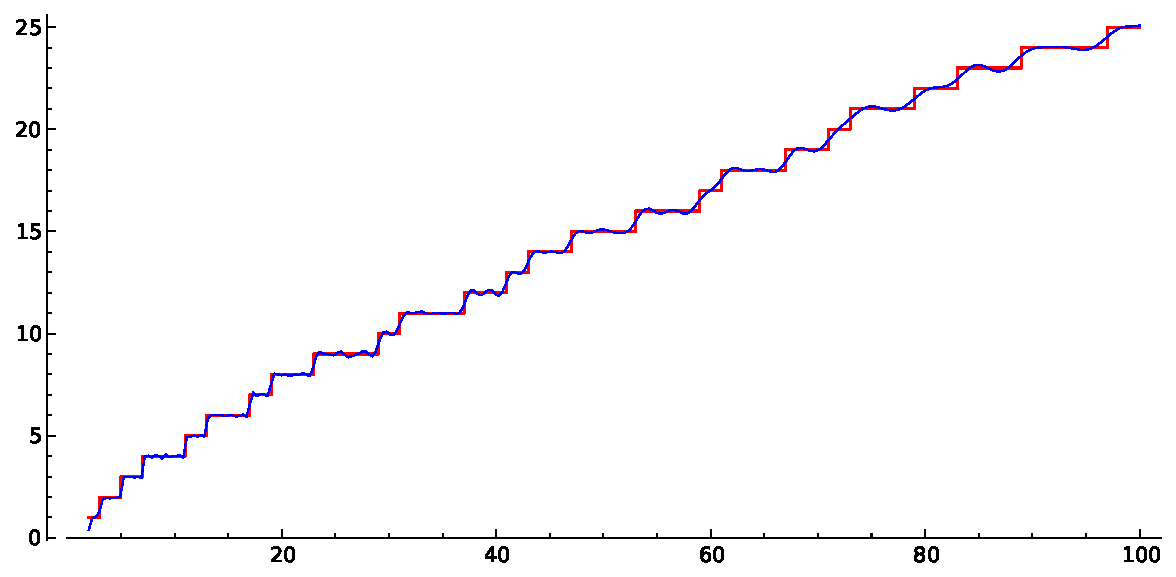
\includegraphics[width=.65\textwidth]{illustrations/Rk_50_2_100}
%... built out of their spectrum:
% cover = use fractal trace with params 0.3 -0.1 0 0
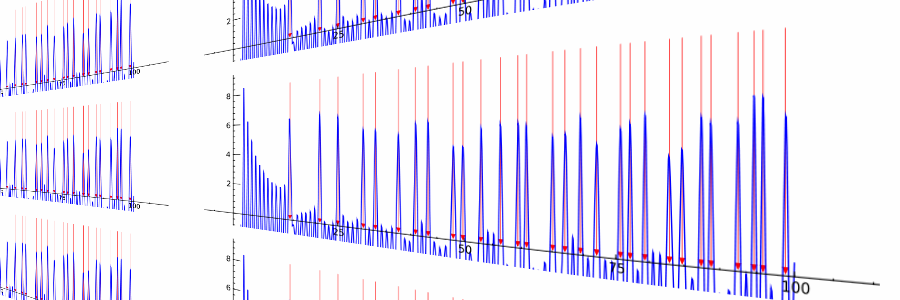
\includegraphics[width=1.1\textwidth]{illustrations/cover}
%$$
%f(t) = -\sum_{\text{prime powers }p^n}{\frac{\log(p)}{p^{n/2}}}\cos(t\log(p^n))
%$$
%\end{center}
}

\usepackage{notes2bib}
\bibliographystyle{amsplain}

\usepackage{hyperref}


\newcommand{\todo}[1]{\par\vspace{1em}{\small---------\\{{\bf To be done:} #1}\\-----------}\par\vspace{1em}}

\begin{document}

\maketitle



% Remove parskip for toc
\setlength{\parskip}{0ex plus 0.5ex minus 0.2ex}

\tableofcontents


% Dutch style of paragraph formatting, i.e. no indents.
\setlength{\parskip}{1.3ex plus 0.2ex minus 0.2ex}

\chapter*{\label{foreword}Foreword}
The \RH{} is one of the great unsolved problems of
mathematics and the reward of \$1,000,000 of {\em Clay Mathematics
  Institute} prize money awaits the person who solves it. But---with
or without money---its resolution is crucial for our understanding of
the nature of numbers.


There are at least four full-length books recently published, written
for a general audience, that have the \RH{} as their main
topic.  A reader of these books will get a fairly rich picture of the
personalities engaged in the pursuit, and of related mathematical and
historical issues. \bibnote{See, e.g., {\em The Music of the Primes} by Marcus du Sautoy.}

This is {\em not} the mission of the book that you now hold in your
hands. We aim---instead---to explain, in as direct a manner as
possible and with the least mathematical background required, what
this problem is all about and why it is so important. For even before
anyone proves this {\em hypothesis} to be true (or false!), just
getting familiar with it and with some of the the ideas behind it, is
exciting.  Moreover, this hypothesis is of crucial importance in a
wide range of mathematical fields; for example, it is a
confidence-booster for computational mathematics: even if the Riemann
Hypothesis is never proved, its truth gives us an excellent sense of
how long certain computer programs will take to run, which, in some
cases, gives us the assurance we need to initiate a computation that
might take weeks or even months to complete.


% I (William Stein) took this very picture in the Princeton common room in 2001!
\ill{sarnak}{0.25}{Peter Sarnak}



Here is how the
Princeton mathematician Peter Sarnak described the broad impact the
Riemann Hypothesis has had:
\begin{quote}
``The Riemann hypothesis is the central problem and it implies many,
many things. One thing that makes it rather unusual in mathematics
today is that there must be over five hundred papers---somebody should
go and count---which start `Assume the Riemann hypothesis,' and
the conclusion is fantastic. And those [conclusions] would then become
theorems ... With this one solution you would have proven five hundred
theorems or more at once.'' \bibnote{See page 222 of
{\em The Riemann hypothesis: the greatest unsolved problem in mathematics} by Karl Sabbagh (2002).}
\end{quote}
% This is from page 106 of the Borwein book, which is just citing Sabbagh.



So, what {\it is} the Riemann Hypothesis?  Below is a {\it first
  description} of what it is about. The task of our book is to develop
the following boxed paragraph into a fuller explanation and to
convince you of the importance and beauty of the mathematics it
represents.  We will be offering, throughout our book, a number of
different---but equivalent---ways of precisely formulating this
hypothesis (we display these in boxes).  When we say that two
mathematical statements are ``equivalent'' we mean that, given the
present state of mathematical knowledge, we can prove that if either
one of those statements is true, then the other is true. The endnotes
will guide the reader to the mathematical literature that establishes
these equivalences.

      \begin{center}
       \shadowbox{ \begin{minipage}{0.91\textwidth}
\mbox{}       \vspace{0.2ex}
       \begin{center}{\bf\large What {\em sort} of Hypothesis is the \RH{}?}\end{center}
       \medskip

Consider the seemingly innocuous series of questions:

\begin{quote}
\begin{itemize}
\item How many prime numbers  (2, 3, 5, 7, 11, 13, 17, $\ldots$) are there less than 100?
\item How many less than 10,000?
\item How many less than 1,000,000?
\end{itemize}

More generally, how many primes are there less than any given number $X$?
\end{quote}

Riemann proposed, a century and half ago, a strikingly
simple-to-describe ``very good approximation'' to the number of
primes less than a given number $X$. We now
see that if we could prove this {\em Hypothesis of Riemann} we would have
the key to a wealth of powerful mathematics. Mathematicians are eager
to find that key.


\vspace{1ex}
\end{minipage}}
      \end{center}

      % I got this from http://www.math.harvard.edu/history/bott/
% Barry says there  is a good picture in the book
% ''the Index Theorem'' that Yau published.
\ill{raoulbott}{0.25}{Raoul Bott (1923--2005)\label{fig:bott}}


A famous mathematician, Raoul Bott, once
said---giving advice to some young mathematicians---that whenever one
reads a mathematics book or article, or goes to a math lecture, one
should aim to come home with something very specific (it can be small,
but should be {\em specific}) that has application to a wider class of
mathematical problem than was the focus of the text or lecture.  If we
were to suggest some possible {\em specific} items to come home with,
after reading our book, three key phrases -- {\bf prime numbers}, {\bf
  square-root accurate}, and {\bf spectrum} -- would head the
list. As for words of encouragement to think hard about the first of
these, i.e., prime numbers, we can do no better than to quote a
paragraph of Don Zagier's classic 12-page exposition, {\em The First
  50 Million Prime Numbers}:

% I took this myself when we were hiking in Oberwolfach once...
\ill{zagier}{.25}{Don Zagier}


\begin{quote}
  ``There are two facts about the distribution of prime numbers of
  which I hope to convince you so overwhelmingly that they will be
  permanently engraved in your hearts. The first is that, [they are]
  the most arbitrary and ornery objects studied by mathematicians:
  they grow like weeds among the natural numbers, seeming to obey no
  other law than that of chance, and nobody can predict where the next
  one will sprout. The second fact is even more astonishing, for it
  states just the opposite: that the prime numbers exhibit stunning
  regularity, that there are laws governing their behavior, and that
  they obey these laws with almost military precision.''
\end{quote}


There are no proofs of anything in this book, and only hints at proofs in the later end-notes. Our exposition is meant to explain the--often quite intuitive-- motivations that have led to the development the fundamental ideas of the subject, as buttressed by numerical experiments, often displayed as graphs. As a result, our book is profusely illustrated, containing over 125 figures,
diagrams, and pictures that accompany the text \bibnote{All of the
  figures were created using the free Sage mathematical
  software \bibnote{The computations for this book were done using
    Sage, which is a free open source mathematical software package
    (\url{http://www.sagemath.org}). The code for the book
    is available at \url{https://github.com/williamstein/rh}.}.
Complete Sage code is available at \url{http://wstein.org/rh}
that can be used to recreate every diagram in this book.
More adventurous readers can
to experiment with the parameters for
the ranges of data illustrated, so as to get an even more
vivid sense of how the numbers ``behave.''} in hopes that readers themselves become inspired to make some numerical experimentation. This will surely become easier for people to do  as mathematical software
advances\footnote{We used \url{http://sagemath.org}
for all computations in this book.}.


  There are  few
mathematical equations in Part~\ref{part1}.  This first portion of our book is intended for readers who are generally interested in, or curious about, mathematical ideas, but who may not have studied any advanced topics. Part~\ref{part1} is devoted to conveying the essence of the Riemann Hypothesis and explaining why it is so intensely pursued. It requires a minimum of mathematical knowledge, and does not,  for example, use calculus, although it would be helpful to know---or to learn on the run---the meaning of  the concept of {\it function}. Given its mission, Part I is meant to be complete, in that it has a beginning, middle, and end.  We hope that our readers who only read Part I will have enjoyed the excitement  of this important piece of mathematics.



    Part~\ref{part2} is for readers who have taken at least one class in calculus, possibly a long time ago.  It is meant as a general preparation for the type of Fourier analysis that will occur in the later parts. The notion of spectrum is key.

    Part~\ref{part3} is for readers who wish to see, more vividly, the link between the placement of prime numbers and (what we call there) the {\it Riemann Spectrum}.

    Part~\ref{part4} requires some familiarity with complex analytic functions, and returns to Riemann's original viewpoint.  In particular it  relates the ``Riemann Spectrum'' that we discuss in Part~\ref{part3} to the {\it nontrivial zeroes of the Riemann's zeta-function}. We also provide a brief sketch of what is the more standard route taken by published expositions of the Riemann Hypothesis.

      The end-notes are meant to link the text to references, but also to provide  more technical commentary with an increasing dependence on mathematical background in the later chapters.  We intend to have a supplementary on-line text that offer a series of exercises that go along with our book.

      We wrote our book over the past decade, but devoted only one week to it each year (a week in August).    At the end of our work-week for the book, each year, we put our draft (mistakes and all) on line to get response from readers. We therefore accumulated much important feedback, corrections, and requests from readers. We thank them infinitely.


\part{The \RH{}\label{part1}}

\numberwithin{equation}{chapter}
\numberwithin{figure}{chapter}
\numberwithin{table}{chapter}

\chapter[Thoughts about numbers]{Thoughts about numbers: ancient, medieval, and modern}

If we are to believe the ancient Greek philosopher Aristotle the early
Pythagoreans thought that the principles governing Number are ``the
principles of all things,'' the concept of Number being more basic than
{\em earth, air, fire, or water}, which were according to ancient tradition
the four building blocks of matter. To think about number is to get
close to the architecture of ``what is.''

So, how far along are we in our thoughts about numbers?


\ill{descartes}{.25}{Ren\'e Descartes}

The French philosopher and mathematician Ren\'e Descartes, almost four
centuries ago, expressed the hope that there soon would be ``almost
nothing more to discover in geometry.'' Contemporary physicists dream
of a final theory \bibnote{See Weinberg's book {\em Dreams of a
    Final Theory: The Search for the Fundamental Laws of Nature}, by
  Steven Weinberg (New York: Pantheon Books, 1992)}.  But despite its
venerability and its great power and beauty, the pure mathematics of
numbers may still be in the infancy of its development, with depths to
be explored as endless as the human soul, and {\it never} a final theory.


% This is from http://en.wikipedia.org/wiki/File:Frans_Hals_-_Portret_van_Ren%C3%A9_Descartes.jpg
% There is a higher resolution scan available there



\ill{dulcinea1}{.2}{Don Quixote and ``his'' Dulcinea del Toboso}

Numbers are obstreperous things. Don Quixote encountered this when he
requested that the ``bachelor'' compose a poem to his lady Dulcinea del
Toboso, the first letters of each line spelling out her name. The
``bachelor'' found




\begin{quote}
  ``a great difficulty in their composition because the number of
  letters in her name was $17$, and if he made four Castilian stanzas
  of four octosyllabic lines each, there would be one letter too many,
  and if he made the stanzas of five octosyllabic lines each, the ones
  called {\em d{\'e}cimas} or {\em redondillas,} there would be three
  letters too few...'' \bibnote{See Chapter IV of the Second Part of the Ingenius Gentleman Don Quixote of La Mancha.}
\end{quote}

``It must fit in, however, you do it,'' pleaded Quixote, not willing to
grant the imperviousness of the number $17$ to division.

% http://www.jus.uio.no/sisu/don_quixote.miguel_de_cervantes/60.html#2068




{\em Seventeen} is indeed a prime number: there is no way of factoring
it as the product of smaller numbers, and this accounts---people tell
us---for its occurrence in some phenomena of nature, as when
the $17$-year cicadas all emerged to celebrate a ``reunion'' of some
sort in our fields and valleys.

\ill{cicada}{.3}{Cicadas emerge every 17 years}
% from http://biology.clc.uc.edu/steincarter/cicadas.htm




Prime numbers, despite their {\em primary} position in our modern
understanding of number, were not specifically doted over in the
ancient literature before Euclid, at least not in the literature that
has been preserved. Primes are mentioned as a class of numbers in the
writings of Philolaus (a predecessor of Plato); they are not mentioned
specifically in the Platonic dialogues, which is surprising
given the intense interest Plato had in mathematical developments; and
they make an occasional appearance in the writings of Aristotle, which
is not surprising, given Aristotle's emphasis on the distinction
between the {\em composite} and the {\em incomposite}. ``The
incomposite is prior to the composite,'' writes Aristotle in Book 13 of
the Metaphysics.


Prime numbers do occur, in earnest, in  Euclid's  {\it Elements}!


% from http://en.wikipedia.org/wiki/File:Euklid-von-Alexandria_1.jpg
\ill{euclid}{.3}{Euclid}


There is an extraordinary wealth of established truths about whole
numbers; these truths provoke sheer awe for the beautiful complexity
of prime numbers. But each of the important new discoveries we make
give rise to a further richness of questions, educated guesses,
heuristics, expectations, and unsolved problems.








\chapter{What are prime numbers?}\label{ch:what_are_primes}

\noindent {\em Primes as atoms. } To begin from the beginning, think
of the operation of multiplication as a bond that ties numbers
together: the equation $2\times 3= 6$ invites us to imagine the number
$6$ as (a molecule, if you wish) built out of its smaller constituents
$2$ and $3$.  Reversing the procedure, if we start with a whole
number, say $6$ again, we may try to factor it (that is, express it as
a product of smaller whole numbers) and, of course, we would
eventually, if not immediately, come up with $6 = 2\times 3$ and
discover that $2$ and $3$ factor no further; the numbers $2$ and $3$,
then, are the indecomposable entities (atoms, if you wish) that
comprise our number.

\ill{factor_tree_6}{.3}{The number $6 = 2\times 3$}


By definition, a {\bf prime number}
(colloquially, {\em a prime}) is a whole number, bigger than $1$, that
cannot be factored into a product of two smaller whole numbers. So,
$2$ and $3$ are the first two prime numbers. The next number along the
line, $4$, is not prime, for $4= 2\times 2$; the number after that,
$5$, is. Primes are, multiplicatively speaking, the building blocks
from which all numbers can be made. A fundamental theorem of
arithmetic tells us that any number (bigger than $1$) can be factored
as a product of primes, and the factorization is {\em unique} except
for rearranging the order of the primes.



For example, if you try to factor $12$ as a product of
smaller numbers---ignoring the order of the factors---there are two
ways to begin to do this:
$$
  12 = 2 \times 6 \qquad\text{ and }\qquad   12 = 3 \times 4
$$
But neither of these ways is a full factorization of $12$, for both
$6$ and $4$ are not prime, so can be themselves factored, and in each
case after changing the ordering of the factors we arrive at:
$$
   12= 2 \times 2 \times 3.
$$

If you try to factor the number $300$, there are many
ways to begin:
$$
  300= 30\times 10\qquad\text{or}\qquad 300 = 6 \times 50
$$
and there are various other starting possibilities. But if you
continue the factorization (``climbing down'' any one of the possible
``factoring trees'') to the bottom, where every factor is a prime
number as in Figure~\ref{fig:factor300}, you always end up with the
same collection of prime numbers \bibnote{See Section~1.1 of
Stein's book {\em Elementary Number Theory: Primes, Congruences, and Secrets} (2008)
for a proof of the ``fundamental theorem of arithmetic'',
which is the statement that every positive
whole number factors uniquely as a product of primes.
This book is freely available at \url{http://wstein.org/ent/}.}:
                 $$300 = 2^2\times 3\times 5^2.$$

\illtwo{factor_tree_300_a}{factor_tree_300_b}{.47}
{Factor trees that illustrates the factorization of 300 as a product of primes.\label{fig:factor300}}

\ill{factor_tree_big}{1}{Factorization tree for the product of the primes up to $29$.\label{factor.tree.big}}


The \RH{} probes the question: how intimately can we know
prime numbers, those {\em atoms} of multiplication?  Prime numbers are
an important part of our daily lives.  For example, anytime we visit a
website and purchase something online, prime numbers having hundreds of
decimal digits are used to keep our bank transactions private.  This
ubiquitous use to which these giant primes are put depends upon a very
simple principle: it is much easier to multiply numbers together than
to factor them. If you had to factor, say, the number $391$ you might
scratch your head for a few minutes before discovering that $391$ is
$17\times 23$. But if you had to multiply $17$ by $23$ you would do it
straightaway.  Offer two primes, say, $P$ and $Q$ each with a few hundred
digits, to your computing machine and ask it to multiply them
together: you will get their product $N = P\times Q$ with its hundreds of digits
in about a microsecond. But present that number $N$ to any
current desktop computer, and ask it to factor $N$, and the computer
will (almost certainly) fail to do the task.
%%%%%%%%%%%%%%%%%%%%%%%%%%%%%%%%%%%%%%%%%%%%%%%%%%%%%%%%%%%%%%%%%%%%%%%%%%%%%%%%%%%%%
\bibnote{{\bf How not to factor the numerator of a Bernoulli number:}

As mentioned in Chapter~\ref{ch:envision}, the coefficient $B_k$ of the linear
term of the polynomial
$$
S_k(n)= 1^k+2^k+3^k+\dots +(n-1)^k
$$
is (up to sign) the $k$-th {\bf Bernoulli number}.  These numbers are
rational numbers and, putting them in lowest terms, their numerators
play a role in certain problems, and their denominators in
others. (This is an amazing story, which we can't go into here!)

One of us (Barry Mazur) in the recent article {\em How can we
  construct abelian Galois extensions of basic number fields?} (see
\url{http://www.ams.org/journals/bull/2011-48-02/S0273-0979-2011-01326-X/})
found himself dealing (for various reasons) with the fraction
$-B_{200}/400$, where $B_{200}$ is the two-hundredth Bernoulli number.
The numerator of this fraction is quite large: it is---hold your
breath---\ $$389\cdot 691\cdot5370056528687 \ \ \ \ {\rm times\ this\
}204-{\rm digit \ number:}
$$\vskip 10pt
$N:=3452690329392158031464109281736967404068448156842396721012$\newline
$\mbox{}\,\,\,\qquad 9920642145194459192569415445652760676623601087497272415557$\newline
$\mbox{}\,\,\,\qquad 0842527652727868776362959519620872735612200601036506871681$\newline
$\mbox{}\,\,\,\qquad 124610986596878180738901486527$
\vskip 10pt  and he {\it incorrectly asserted} that it was prime.  Happily, Bartosz Naskr\c{e}cki spotted this error: our $204$-digit $N$ is {\it not} prime.
% Note, according to http://perso.telecom-paristech.fr/~cappe/local/latex/accents.pdf
% the accent I get with \c{e} is ``NOTE: This is technically incorrect.  The accent should be reversed in orientation,
% but there is currently no such accent in plain TEX or LATEX.''

How did he know this?  By using the most basic test in the repertoire
of tests that we have available to check to see whether a number is
prime: we'll call it the ``{\bf Fermat $2$-test.}'' We'll first give a
general explanation of this type of test before we show how $N$ {\it
  fails the Fermat $2$-test.}


The starting idea behind this test is the famous result known as {\em
  Fermat's Little Theorem} where the ``little'' is meant to
alliteratively distinguish it from you-know-what.
\begin{theorem}[Fermat's Little Theorem]
If $p$ is a prime number, and $a$ is any number relatively prime to $p$ then $a^{p-1} - 1$ is divisible by $p$.
\end{theorem}
A good exercise is to try to prove this, and a one-word hint that might lead you to one of the many proofs of it is
{\em induction}.\footnote{Here's the proof:
$$(N+1)^p \equiv N^p +1 \equiv (N+1),$$
where the first equality is the binomial theorem and the second
equality is induction.}

 Now we are going to use this as a criterion, by---in effect---restating it in what logicians would call  its {\it contrapositive}:
 \begin{theorem}[The Fermat $a$-test]
If $M$ is a positive integer, and $a$ is any number relatively prime to $M$ such that  $a^{M-1} - 1$ is {\it not} divisible by $M$, then $M$ is {\it not} a prime.
\end{theorem}

Well, Naskr\c{e}cki computed $2^{N-1}-1$  (for the $204$-digit $N$ above)   and saw that
it is {\it not} divisible by $N$.{\footnote{and has a residue of $3334581100595953025153969739282790317394606677381970645616725285996925
66100005682$\newline$92727335792620957159782739813115005451450864072425835484898
5651127636929707992693354028195076056916221$\newline$73717318335512037458$ after division by $N$.}}
Ergo, our $N$ fails the  Fermat $2$-test so is {\it not} prime.

But then, given that it is so ``easy'' to see that $N$ is not prime, a
natural question to ask is: what, in fact, is its prime factorization?
This---it turns out---isn't so easy to determine;
Naskr\c{e}cki devoted $24$ hours of computer time setting standard factorization
algorithms on the task, and that was not sufficient time to resolve
the issue.  The factorization of the numerators of general Bernoulli
numbers is the subject of a very interesting web site of Samuel
Wagstaff (\url{http://homes.cerias.purdue.edu/~ssw/bernoulli}).
Linked to this web page one finds
(\url{http://homes.cerias.purdue.edu/~ssw/bernoulli/composite}) which gives
a list of composite numbers whose factorizations have resisted all
attempts to date.  The two-hundredth Bernoulli number is 12th on the list.

 The page
\url{http://en.wikipedia.org/wiki/Integer_factorization_records} lists
record challenge factorization, and one challenge that was completed
in 2009 involves a difficult-to-factor number with 232 digits; its
factorization was completed by a large team of researchers and took around
2000 years of CPU time.  This convinced us that
with sufficient motivation  it would be possible to factor $N$, and so we
asked some leaders in the field to try.   They succeeded!
\begin{quote}\sf
Factorisation of B200

by Bill Hart on 4 Aug 05, 2012 at 07:24pm

We are happy to announce the factorization of the numerator of the 200th
Bernoulli number:

\begin{align*}
N &= 389 \cdot 691 \cdot 5370056528687 \cdot c_{204}\\
c_{204} &= p_{90} \cdot p_{115}\\
p_{90}  &= 149474329044343594528784250333645983079497454292\\
        &= 838248852612270757617561057674257880592603\\
p_{115} &= 230988849487852221315416645031371036732923661613\\
        &= 619208811597595398791184043153272314198502348476\\
        &= 2629703896050377709
\end{align*}

The factorization of the 204-digit composite was made possible with the help
of many people:
\begin{itemize}
\item William Stein and Barry Mazur challenged us to factor this number
\item Sam Wagstaff maintains a table of factorizations of numerators of Bernoulli
  numbers at \url{http://homes.cerias.purdue.edu/~ssw/bernoulli/bnum}. According
  to this table, the 200th Bernoulli number is the 2nd smallest index with
  unfactored numerator (the first being the 188th Bernoulli number)
\item Cyril Bouvier tried to factor the c204 by ECM up to 60-digit level, using
  the TALC cluster at Inria Nancy - Grand Est
\item {\sf yoyo@home} tried to factor the c204 by ECM up to 65-digit level, using the
  help of many volunteers of the distributed computing platform
  \url{http://www.rechenkraft.net/yoyo/}.
 after ECM was unsuccessful, we decided to factor the c204 by GNFS
\item Many people at mersenne forum helped for the polynomial selection. The best
  polynomial was found by Shi Bai, using his implementation of Kleinjung's
  algorithm in CADO-NFS:
  \url{http://www.mersenneforum.org/showthread.php?p=298264#post298264}
 sieving was performed by many volunteers {\sf NFS@home}, thanks to Greg
  Childers. See \url{http://escatter11.fullerton.edu/nfs} for more details {\sf NFS@home}
  This factorization showed that such a distributed effort might be feasible for a
  new record GNFS factorization, in particular for the polynomial selection.
  This was the largest GNFS factorization performed by {\sf NFS@home} to date,
  the second largest being $2^{1040}+1$ at 183.7 digits.
\item Two independent runs of the filtering and linear algebra were done: one by Greg
  Childers with msieve (\url{http://www.boo.net/~jasonp/qs.html}) using a 48-core
  cluster made available by Bill Hart, one by Emmanuel Thomé and Paul
  Zimmermann with CADO-NFS (\url{http://cado-nfs.gforge.inria.fr/}), using the Grid
  5000 platform.
\item The first linear algebra run to complete was the one with CADO-NFS, thus we
  decided to stop the other run.
\end{itemize}

Bill Hart
\end{quote}

Verify the above in Sage as follows: \\

{\sf
sage: p90 = 1494743290443435945287842503336459830794974542928382\textbackslash\\
48852612270757617561057674257880592603\\
sage: p115 = 230988849487852221315416645031371036732923661613619\textbackslash\\
2088115975953987911840431532723141985023484762629703896050377709\\
sage: c204 = p90 * p115\\
sage: 389 * 691 * 5370056528687 * c204 == -numerator(bernoulli(200))\\
True\\
sage: is\_prime(p90), is\_prime(p115), is\_prime(c204)\\
(True, True, False)
}
}
\bibnote{\label{bibnote:factor}
Given an integer $n$, there are
many algorithms available for trying to write $n$ as a product of
prime numbers.  First we can apply {\em trial division}, where we
simply divide $n$ by each prime $2, 3, 5, 7, 11, 13, \ldots$ in turn,
and see what small prime factors we find (up to a few digits).  After
using this method to eliminate as many primes as we have patience to
eliminate, we typically next turn to a technique called {\em Lenstra's
  elliptic curve method}, which allows us to check $n$ for
divisibility by bigger primes (e.g., around 10--15 digits).  Once
we've exhausted our patience using the elliptic curve method, we would
next hit our number with something called the {\em quadratic sieve},
which works well for factoring numbers of the form $n=pq$, with $p$
and $q$ primes of roughly equal size, and $n$ having less than 100
digits (say, though the 100 depends greatly on the implementation).
All of the above algorithms---and then some---are implemented in Sage,
and used by default when you type {\tt factor(n)} into Sage. Try
typing {\tt factor(some number, verbose=8)} to see for yourself.

If the quadratic sieve fails, a final recourse is to run the {\em
  number field sieve} algorithm, possibly on a supercomputer.  To give
a sense of how powerful (or powerless, depending on perspective!)  the
number field sieve is, a record-setting factorization of a general
number using this algorithm is the factorization of a 232 digit number
called RSA-768:

$
n = 12301866845301177551304949583849627207728535695953347921973224521\\
517264005072636575187452021997864693899564749427740638459251925573263\\
034537315482685079170261221429134616704292143116022212404792747377940\\
80665351419597459856902143413
$
\par\noindent{}which factors as $pq$, where\par\noindent{}
$
 p = 334780716989568987860441698482126908177047949837137685689124313889\\
82883793878002287614711652531743087737814467999489
$
\par\noindent{}and\par\noindent{}
$
q = 367460436667995904282446337996279526322791581643430876426760322838\\
15739666511279233373417143396810270092798736308917.
$
\par\noindent{}We encourage you to try to
factor $n$ in Sage, and see that it fails.
Sage does not currently (as of 2011) include an implementation of the
number field sieve algorithm, though there are some free implementations
currently available (see \url{http://www.boo.net/~jasonp/qs.html}).
}

%%%%%%%%%%%%%%%%%%%%%%%%%%%%%%%%%%%%%%%%%%%%%%%%%%%%%%%%%%%%%%%%%%%%%%%%%%%%%%%%%%%%%




%We illustrate this in Sage:
% \begin{lstlisting}[]
% sage: n = ZZ.random_element(10^500)
% sage: m = ZZ.random_element(10^500)
% sage: timeit('n*m')
% 1.51 microseconds per loop
% sage: timeit('n*m')
% 2.33 microseconds per loop
% sage: factor(n*m)
% [wait forever]
% \end{lstlisting}}.
The safety of much
encryption depends upon this ``guaranteed'' failure! \bibnote{Nobody has ever
  published a {\em proof} that there is no fast way to factor
  integers.  This is an article of ``faith'' among some
  cryptographers.}

If we were latter-day number-phenomenologists we might revel in the
discovery and proof that
$$
  p=2^{43,112,609}-1 = 3164702693\ldots\ldots\text{\small (millions of digits)}\ldots\ldots6697152511
$$
is a prime number, this number having $12{,}978{,}189$ digits!  This
prime, which was discovered on August 23, 2008 by the GIMPS project
(see \bibnote{The GIMPS project website is \url{http://www.mersenne.org/}.}),
is the first prime ever found with more than ten million digits,
though it is not the largest prime currently known.

Now $2^{43,112,609}-1$ is quite a hefty number! Suppose someone came
up to you saying ``surely $p = 2^{43,112,609}-1$ is the largest prime
number!'' (which it is not) how might you convince that person that
he or she is wrong without explicitly exhibiting a larger prime?
\bibnote{We can use Sage (at \url{http://sagemath.org}) to quickly compute the ``hefty
number'' $p = 2^{43,112,609}-1$.  Simply type
{\tt p = 2\^{}43112609 - 1} to instantly compute $p$.
In what sense have we {\em computed} $p$?  Internally, $p$ is now
stored in base $2$ in the computer's memory; given the special form of
$p$ it is not surprising that it took little time to compute.  Much more
challenging is to compute all the base 10 digits of $p$, which takes
a few seconds: {\tt d = str(p)}.
Now type {\tt d[-50:]} to see the last 50 digits of $p$.
To compute the sum $58416637$ of the digits of $p$ type {\tt sum(p.digits())}.
}


Here is a neat---and, we hope, convincing---strategy to show there are
prime numbers even larger than $p = 2^{43,112,609} - 1$. Imagine
forming the following humongous number: let $M$ be the product of all
prime numbers up to and including $p = 2^{43,11,2609} - 1$.  Now go
one further than $M$ by taking the next number $N=M+1$.


OK, even though this number $N$ is wildly large, it is either a prime
number itself---which would mean that there would indeed be a prime
number larger than $p=2^{43,112,609} - 1$, namely $N$; or in any event it is
surely divisible by some prime number, call it $P$.

Here, now, is a way of seeing that this $P$ is bigger than $p$: Since
every prime number smaller than or equal to $p$ divides $M$, these
prime numbers cannot divide $N= M+1$ (since they divide $M$ evenly, if
you tried to divide $N=M+1$ by any of them you would get a remainder
of $1$).  So, since $P$ does divide $N$ it must not be any of the
smaller prime numbers: $P$ is therefore a prime number bigger than $p=
2^{43,112,609}-1$.

This strategy, by the way, is not very new: it is, in fact, well over
two thousand years old, since it already occurred in Euclid's {\em
  Elements}. The Greeks did know that there are infinitely many prime
numbers and they showed it via the same method as we showed that our
$p = 2^{43,112,609} - 1$ is not the largest prime number.

Here is the argument again, given very succinctly:
Given primes $p_1, \ldots, p_m$, let $n=p_1 p_2 \cdots p_m +
1$.  Then $n$ is divisible by some prime not equal to any $p_i$,
so there are more than $m$ primes.

You can think of this strategy as a simple game that you can
play. Start with any finite bag of prime numbers (say the bag that
only contains one prime, the prime $2$). Now each ``move'' of the game
consists of multiplying together all the primes you have in your bag
to get a number $M$, then adding $1$ to $M$ to get the even larger
number $N=M+1$, then factoring $N$ into prime number factors, and then
including all those new prime numbers in your bag. Euclid's proof
gives us that we will---with each move of this game---be finding more
prime numbers: the bag will increase. After, say, a million moves our
bag will be guaranteed to contain more than a million prime numbers.

For example, starting the game with your bag containing
only one prime number $2$, here is how your bag grows with after
successive moves of the game:

$\mbox{}\qquad\{2\}$
\newline
$\mbox{}\qquad\{2,3\}$
\newline
$\mbox{}\qquad\{2,3, 7\}$
\newline
$\mbox{}\qquad\{2,3, 7, 43\}$
\newline
$\mbox{}\qquad\{2,3, 7, 43, 13, 139\}$
\newline
$\mbox{}\qquad\{2,3, 7, 43, 13, 139, 3263443\}$
\newline
$\mbox{}\qquad\{2,3, 7, 43, 13, 139, 3263443,  547, 607, 1033, 31051\}$
\newline
$\mbox{}\qquad\{2,3, 7, 43, 13, 139, 3263443,  547, 607, 1033, 31051, 29881, 67003,\\
\mbox{}\qquad\qquad\qquad 9119521, 6212157481\}$
\newline
\mbox{}\qquad{}etc. \bibnote{The sequence of prime numbers we find by this
procedure is discussed in more detail with references
in the Online Encyclopedia of Integer Sequences \url{http://oeis.org/A126263}.}

Though there are infinitely many primes, actually finding them is a
major challenge.  In the 1990s, the Electronic Frontier Foundation
\url{http://www.eff.org/awards/coop} offered a \$100,000 cash reward
to the first group to find a prime with at least 10,000,000 decimal
digits (the record prime $p$ above won this prize \bibnote{%
See \url{http://www.eff.org/press/archives/2009/10/14-0}.
Also the 46th Mersenne prime was declared by Time Magazine to be
one of the top 50 best ``inventions'' of 2008: \url{http://www.time.com/time/specials/packages/article/0,28804,1852747_1854195_1854157,00.html}.}), and offers
another \$150,000 cash prize to the first group to find a prime with
at least 100,000,000 decimal digits.


The number $p= 2^{43,112,609} - 1$  was for a time
the largest prime known, where by
``know'' we mean that we know it so explicitly that we can {\em
  compute} things about it.  For example, the last two digits of $p$
are both 1 and the sum of the digits of $p$ is 58,416,637.\label{sumdigits}  Of course $p$ is not
the largest prime number since there are infinitely many primes, e.g.,
the next prime $q$ after $p$ is a prime.  But there is no known way
to efficiently compute anything interesting about $q$.  For example,
what is the last digit of $q$ in its decimal expansion?


\chapter{``Named'' Prime Numbers}
Prime numbers come in all sorts of shapes, some more convenient to
deal with than others.  For example, the number we have been talking
about, $$p = 2^{43,112,609}-1,$$ is given to us, by its very notation,
in a striking form; i.e., {\it one less than a power of $2$}. It is no
accident that the largest ``currently known'' prime number has such a
form.  This is because there are special techniques we can draw on to
show primality of a number, if it is one less than a power of $2$
and---of course---if it also happens to be prime.  The primes of that
form have a name, {\it Mersenne Primes}, as do the primes that are
{\it one more than a power of $2$}, those being called {\it Fermat
  Primes}.
\bibnote{
In contrast to the situation with factorization, testing integers of
this size (e.g., the primes $p$ and $q$) for primality is relatively
easy.  There are fast algorithms that can tell whether or not any
random thousand digit number is prime in a fraction of
second. Try for yourself using the Sage command {\tt is\_prime}.
For example, if $p$ and $q$ are as in endnote~\ref{bibnote:factor}, then
{\tt is\_prime(p)} and {\tt is\_prime(q)} quickly output True
and {\tt is\_prime(p*q)} outputs False.  However, if you type
{\tt factor(p*q, verbose=8)}  you can watch as Sage tries
forever and fails to factor $pq$.}

Here are two exercises that you might try to do, if this is your first
encounter with primes that differ from a power of $2$ by $1$:

\begin{enumerate}
\item Show that if a number of the form $M=2^n-1$ is prime, then the
  exponent $n$ is also prime. [Hint: This is equivalent to proving
  that if $n$ is composite, then $2^n-1$ is also composite.]
  For example: $ 2^2-1= 3, 2^3-1= 7$ are
  primes, but $2^4-1=15$ is not.  So {\it Mersenne primes} are numbers
  that are
  \begin{itemize}
    \item of the form $$2^{\rm prime\ number} -1,$$ and
    \item are themselves prime numbers.
  \end{itemize}

\item Show that if a number of the form $F=2^n+1$ is prime, then the
  exponent $n$ is a power of two.  For example: $ 2^2+1= 5$ is prime,
  but $2^3+1= 9$ is not.  So {\it Fermat primes} are numbers that
  are
  \begin{itemize}
     \item of the form $$2^{\rm power\ of\ two} +1,$$ and
     \item are themselves prime numbers.
  \end{itemize}
\end{enumerate}


Not all numbers of the form $2^{\rm prime\ number} -1$ or of the form
$2^{\rm power\ of\ two} +1$ are prime. We currently know only finite
many primes of either of these forms. How we have come to know what we
know is an interesting tale.  See, for example, \url{http://www.mersenne.org/}.

%\ill{sieve_boxes_100}{0.7}{Sieve of Eratosthenes\label{fig:erat}}

\chapter{Sieves}\label{ch:sieves}

Eratosthenes, the mathematician from Cyrene (and later, librarian at
Alexandria) explained how to {\em sift} the prime numbers from the
series of all numbers: in the sequence of numbers,
$$2\ \ 3\ \ 4 \ \ 5\ \ 6\ \ 7\ \ 8\ \ 9\ \ 10\ \ 11
\ \ 12\ \ 13\ \ 14\ \ 15\ \ 16\ \ 17\ \ 18\ \ 19\ \ 20\ \ 21\ \ 22\ \ 23\ \ 24\ \ 25\ \ 26,$$
for example, start by circling the $2$ and crossing out all the other
multiples of $2$.  Next, go back to the beginning of our sequence of
numbers and circle the first number that is neither circled nor
crossed out (that would be, of course, the $3$), then cross out all
the other multiples of $3$.  This gives the pattern: go back again to
the beginning of our sequence of numbers and circle the first number
that is neither circled nor crossed out; then cross out all of its
other multiples.  Repeat this pattern until all the numbers in our
sequence are either circled, or crossed out, the circled ones being
the primes.

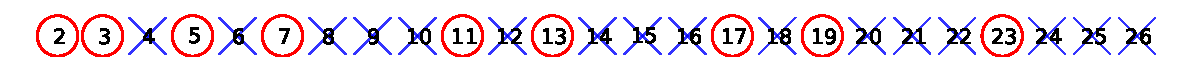
\includegraphics[width=\textwidth]{illustrations/circled_primes}

In Figures~\ref{fig:erat2}--\ref{fig:erat2357} we use the primes $2$,
$3$, $5$, and finally $7$ to sieve out the primes up to 100, where instead of
crossing out multiples we grey them out, and instead of circling
primes we color their box red.

\ill{sieve100-2}{.8}{Using the prime 2 to sieve for primes up to 100\label{fig:erat2}}
Since all the even numbers greater than two are
eliminated as being composite numbers and not primes they appear as
gray in Figure~\ref{fig:erat2}, but none of the odd numbers are eliminated so they
still appear in white boxes.

\ill{sieve100-3}{.8}{Using the primes 2 and 3 to sieve for primes up to 100\label{fig:erat23}}
\ill{sieve100-5}{.8}{Using the primes 2,3,5 to sieve for primes up to 100\label{fig:erat235}}
Looking at Figure~\ref{fig:erat235}, we see that for all but
six numbers up to 100 we have  (after sieving by 2,3, and 5) determined
which are primes and which composite.

\ill{sieve100-7}{.8}{Using the primes 2,3,5,7 to sieve for primes up to 100\label{fig:erat2357}}

Finally, as in Figure~\ref{fig:erat2357},
sieving by 2,3,5, and 7 we have determined which are primes for all but two numbers.
\bibnote{In Sage, the
function {\tt prime\_range} enumerates primes in a range, e.g.,
{\tt prime\_range(50)}
outputs the primes up to $50$
and {\tt prime\_range(50,100)}
outputs the primes between $50$ and $100$.
Typing {\tt prime\_range(10\^{}8)}
in Sage enumerates the primes up to a hundred million in around a second.
You can also enumerate primes up to a billion by typing {\tt v=prime\_range(10\^{}9)}, but this will use
a large amount of memory, so be careful not to crash your computer
if you try this.  Notice that there are $\pi(10^9) = 50{,}847{,}534$ primes up to a billion
by then typing {\tt len(v)}.
You can also compute $\pi(10^9)$ directly, without enumerating all primes,
using the command {\tt prime\_pi(10\^{}9)}.
This is much faster since it uses some clever counting tricks to find the
number of primes without actually listing them all.

In Chapter~\ref{sec:tinkering} we tinkered with the staircase of
primes by first counting both primes and prime powers.    It turns out
that there are comparatively few prime powers that are not prime.
Up to $10^8$, only $1{,}405$ of the $5{,}762{,}860$ prime powers are not themselves primes.
To see this, first enter
{\tt a~=~prime\_pi(10\^{}8); pp~=~len(prime\_powers(10\^{}8))}.
Typing {\tt (a,~pp,~pp-a)} then outputs the triple
{\tt (5761455, 5762860, 1405)}.}


% GIVEN WHAT IS ABOVE, THIS IS SILLY.
%Especially if you have had little experience with math, may I suggest
%that you actually follow Eratosthenes' lead, and perform the repeated
%circling and crossing-out to watch the primes up to 100 emerge, intriguingly
%staggered through our sequence of numbers,
%$$2\ \ 3\ \ \bullet \ \ 5\ \ \bullet\ \ 7\ \ \bullet\ \ \bullet\ \ \bullet\ \ 11
%\ \ \bullet\ \ 13\ \ \bullet\ \ \bullet\ \ \bullet\ \ 17\ \ \bullet\ \ 19\ \ \bullet\ \ \bullet\ \
%\bullet\
%\ 23\ \ \bullet\ \ \bullet\ \ \bullet\ \  \bullet\ \ \bullet\ 29,\dots $$
%

%


\chapter[Questions about primes]{Questions about primes that any person might ask}

We become quickly stymied when we ask quite elementary questions about
the spacing of the infinite series of prime numbers.

For example, {\em are there infinitely many pairs of primes whose
  difference is $2$?}  The sequence of primes seems to be rich in such
pairs $$5-3 =2,\ \ \ 7-5=2,\ \ \ 13-11=2,\ \ \ 19-17 =2,$$ and we know
that there are loads more such pairs (see \bibnote{For example, according to
\url{http://oeis.org/A007508} there are
$10{,}304{,}185{,}697{,}298$ such pairs less than
$10{,}000{,}000{,}000{,}000{,}000$.}) but the answer to our question,
{\em are there infinitely many?}, is not known. The conjecture that there are infinitely many such pairs of primes (``twin primes" as they are called) is known as the {\it Twin Primes Conjecture}.
{\em Are there
  infinitely many pairs of primes whose difference is $4$, $6$?}  Answer:
equally unknown.
Nevertheless there is very exciting recent work in this direction, specifically,
Yitang Zhang proved that there are infinitely many pairs of primes that differ
by no more than $7\times 10^7$. For a brief account of this, see the wikipedia entry \url{http://en.wikipedia.org/wiki/Yitang_Zhang}, and for a popular report  about developments following Zhang's breakthrough result (we know now, thanks to results of James Maynard and others, that there are infinitely many pairs of primes that differ
by no more than $252$) see \url{https://www.simonsfoundation.org/quanta/20131119-together-and-alone-closing-the-prime-gap/} and for further work
\url{http://michaelnielsen.org/polymath1/index.php?title=Bounded_gaps_between_primes}.

{\em Is every even number greater than $2$ a sum of
  two primes?}  Answer: unknown. {\em Are there infinitely many primes
  which are $1$ more than a perfect square?}  Answer: unknown.

\ill{zhang}{0.25}{Yitang Zhang\label{fig:zhang}}



Remember the Mersenne prime $p= 2^{43,112,609}-1$? and how we
proved---by pure thoughts---that there must be
a prime $P$ larger than that? Suppose, though, someone
asked us whether there was a {\it Mersenne Prime} larger than this
$p$: that is, {\em is there a prime number of the form $$2^{\rm some\
  prime\ number}-1$$ bigger than $p= 2^{43,112,609}-1$?} Answer:
For many years we did not know; however, in 2013 Curtis Cooper discovered
the even bigger Mersenne prime $2^{57,885,161}-1$, with a whopping
17,425,170 digits!  Again we can ask if there is a Mersenne
prime larger than Cooper's.  Answer: we do not know.
It is possible that there are infinitely many Mersenne primes
but we're far from being able to answer such questions.

% from http://www.york.ac.uk/depts/maths/histstat/people/mersenne.gif
\ill{mersenne}{.3}{Mersenne}



{\em Is there some neat formula giving the next prime?} More
specifically, {\em If I give you a number $N$, say $N=$ one million,
  and ask you for the first number after $N$ that is prime, is there a
  method that answers that question without, in some form or other,
  running through each of the successive odd numbers after $N$ rejecting
  the nonprimes until the first prime is encountered?}  Answer:
unknown.


%%%%%%%%%%%%%%%

One can think of many ways of ``getting at'' some understanding of the
placement of prime numbers among all numbers.  Up to this point we have
been mainly just counting them, trying to answer the question ``how
many primes are there up to $X$?''  and we have begun to get some feel
for the numbers behind this question, and especially for the current
``best guesses'' about estimates.


What is wonderful about this subject is that people attracted to it
cannot resist asking questions that lead to interesting, and sometimes
surprising numerical experiments. Moreover, given our current state of
knowledge, many of the questions that come to mind are still
unapproachable: we don't yet know enough about numbers to answer them.
But {\it asking interesting questions} about the mathematics that you
are studying is a high art, and is probably a necessary skill to
acquire, in order to get the most enjoyment---and understanding---from
mathematics.  So, we offer this challenge to you:

Come up with with your own question about primes that
 \begin{itemize}
 \item     is interesting to you,
  \item    is not a question whose answer is known to you,
 \item     is not a question that you've seen before; or at least not exactly,
  \item    is a question about which you can begin to make numerical investigations.
 \end{itemize}
If you are having trouble coming up with a question, read on for more
examples that  provide further motivation.

\chapter{Further questions about primes\label{ch:further}}

In celebration of Yitang Zhang's recent result, let us consider more of the numerics
regarding {\em gaps} between one prime and the next, rather than the tally
of all primes. Of course, it is no fun at all to try to guess how many
pairs of primes $p, q$ there are with gap $q-p$ equal to a fixed odd
number, since the difference of two odd numbers is even.  The fun,
though, begins in earnest if you ask for pairs of primes with
difference equal to $2$ (these being called {\em twin primes}) for it
has long been guessed that there are infinitely many such pairs of
primes, but no one has been able to prove this yet.

\begin{quote} As of 2014, the largest known twin primes are
$$3756801695685\cdot 2^{666669} \pm 1$$
These enormous primes have $200700$ digits each (see \bibnote{See \url{http://primes.utm.edu/largest.html\#twin} for the top ten
largest known twin primes.}).
\end{quote}


Similarly, it interesting to consider primes $p$ and $q$
with difference $4$, or $8$, or---in fact---any even number
$2k$. That is, people have guessed that there are infinitely many
pairs of primes with difference $4$, with difference $6$, etc. but
none of these guesses have yet been proved.





So, define
$$
  \Gap_{k}(X)
$$
to be the number of pairs of {\em consecutive} primes $(p,q)$ with
$q<X$ that have ``gap $k$'' (i.e., such that their difference $q-p$ is
$k$).  Here $p$ is a prime, $q>p$ is a prime, and there are no primes
between $p$ and $q$.  For example, $\Gap_2(10) = 2$, since the pairs
$(3,5)$ and $(5,7)$ are the pairs less than $10$ with gap $2$,
and $\Gap_{4}(10)=0$ because despite $3$ and $7$ being separated
by $4$, they are not consecutive primes.
See Table~\ref{tab:gap} for various values of $\Gap_{k}(X)$ and
Figure~\ref{fig:primegapdist} for the distribution of prime gaps for
$X=10^7$.


\begin{table}[H]\centering
\caption{Values of $\Gap_{k}(X)$ \label{tab:gap}}
\vspace{1em}

{\small
\begin{tabular}{|l|c|c|c|c|c|c|}\hline
$X$ & $\Gap_{2}(X)$ & $\Gap_{4}(X)$& $\Gap_{6}(X)$ & $\Gap_{8}(X)$ &
 $\Gap_{100}(X)$ &   $\Gap_{252}(X)$\\\hline

$10$ & 2 & 0 & 0 & 0 & 0 & 0\\\hline
$10^{2}$ & 8 & 7 & 7 & 1 & 0 & 0\\\hline
$10^{3}$ & 35 & 40 & 44 & 15 & 0 & 0\\\hline
$10^{4}$ & 205 & 202 & 299 & 101 & 0 & 0\\\hline
$10^{5}$ & 1224 & 1215 & 1940 & 773 & 0 & 0\\\hline
$10^{6}$ & 8169 & 8143 & 13549 & 5569 & 2 & 0\\\hline
$10^{7}$ & 58980 & 58621 & 99987 & 42352 & 36 & 0\\\hline
$10^{8}$ & 440312 & 440257 & 768752 & 334180 & 878 & 0\\\hline

\end{tabular}
}
\end{table}

 The recent results of Zhang as sharpened by Maynard (and others) we mentioned above tell us that for  at least one even number $k$ among the  even numbers $k \le 252$,    $\Gap_{k}(X)$ goes to infinity as $X$ goes to infinity. One expects that this happens for {\it all} even numbers $k$. We expect this as well, of course, for $\Gap_{252}(X)$ despite what might be misconstrued as discouragement by the above data.

\ill{primegapdist}{1}{Frequency histogram showing the distribution of
  prime gaps of size $\leq 50$ for all primes up to $10^7$.  Six is
  the most popular gap in this data.  The vertical axis labels
  such as ``6e4'' mean $6\cdot 10^4=60{,}000$.
\label{fig:primegapdist}}


\ill{primegap_race}{1}{Plots of $\Gap_k(X)$ for $k=2,4,6,8$.  Which wins?}

Here is yet another question that deals with the spacing of prime
numbers that we do not know the answer to:

{\em Racing Gap $2$,  Gap $4$, Gap $6$, and Gap $8$ against each other:}

\begin{quote}
  Challenge: As $X$ tends to infinity which of $\Gap_2(X)$,
  $\Gap_4(X)$,
  $\Gap_6(X),$ or $\Gap_8(X)$ do you think will grow faster? How
  much would you bet on the truth of your guess? \bibnote{%
    Hardy and Littlewood give a nice conjectural answer to such
    questions about gaps between primes.  See Problem {\bf A8} of
    Guy's book {\em Unsolved Problems in Number Theory} (2004).
Note that Guy's book discusses counting the number $P_k(X)$ of pairs of
primes up to $X$ that differ by a fixed even number $k$; we have
$P_k(X)\geq \Gap_k(X)$, since for $P_k(X)$ there is no requirement
that the pairs of primes be consecutive.}
\end{quote}









Here is a curious question that you can easily begin to check out for
small numbers. We know, of course, that the {\em even} numbers and the
{\em odd} numbers are nicely and simply distributed: after every odd
number comes an even number, after every even, an odd, there are an
equal number of odd number as even numbers less than any given odd
number, and there may be nothing else of interest to say about the
matter.  Things change considerably, though, if we focus our
concentration on {\em multiplicatively even} numbers and {\em
  multiplicatively odd} numbers.


A {\bf multiplicatively even} number is one that can be expressed as a
product of {\em an even number of} primes; and a {\bf multiplicatively
  odd} number is one that can be expressed as a product of {\em an odd
  number of} primes.  So, any prime is multiplicatively odd, the
number $4 = 2\cdot 2$ is multiplicatively even, and so is $6=2\cdot
3$, $9=3\cdot 3$, and $10= 2\cdot 5$; but $12=2\cdot 2\cdot 3$ is
multiplicatively odd.   Below we list the numbers up to 25, and underline
and bold  the multiplicatively odd numbers.
\begin{center}
1\, {\bf \underline{2}}\, {\bf \underline{3}}\, 4\, {\bf
\underline{5}}\, 6\, {\bf \underline{7}}\, {\bf \underline{8}}\, 9\,
10\, {\bf \underline{11}}\, {\bf \underline{12}}\, {\bf
\underline{13}}\, 14\, 15\, 16\, {\bf \underline{17}}\, {\bf
\underline{18}}\, {\bf \underline{19}}\, {\bf \underline{20}}\, 21\,
22\, {\bf \underline{23}}\, 24\, 25
\end{center}


 Table~\ref{tab:evenodddata} gives some data:

 \begin{table}[H] \caption{Count of multiplicatively odd and
    multiplicatively even positive numbers $\le X$\label{tab:evenodddata}}
\vspace{1ex}
\centering
 {\small
\begin{tabular}{|l|r|r|r|r|r|r|r|r|r|r|r|r|r|r|r|r|}
\hline
$X$ & 1 & 2 & 3 & 4 & 5  & 6 & 7 & 8 & 9 & 10 & 11 & 12 & 13 & 14 & 15 & 16  \\ \hline\hline
m. odd & 0 & 1 & 2 & 2 & 3  & 3 & 4 & 5 & 5 & 5 & 6 & 7 & 8 & 8 & 8 & 8 \\ \hline
m. even & 1 & 1 & 1 & 2 & 2  & 3 & 3 & 3 & 4 & 5 & 5 & 5 & 5 & 6 & 7 & 8 \\ \hline
\end{tabular}}
\end{table}


   Now looking at this data, a natural, and simple, question to ask about the concept of multiplicative {\em oddness} and {\em evenness} is:

   \noindent {\em Is there some $X\ge 2$ for which there are more
     multiplicatively even numbers less than or equal to $X$ than
     multiplicatively odd ones?}

   Each plot in Figure~\ref{fig:liouville} gives the number of
   multiplicatively odd numbers between $2$ and $X$ minus the number
   of multiplicatively even numbers between $2$ and $X$, for $X$ equal
   to 10, 100, 1000, 10000, 100000, and 1000000. The above question
   asks whether these graphs would, for sufficiently large $X$, ever
   cross the $X$-axis.

 \begin{figure}[H]
\centering
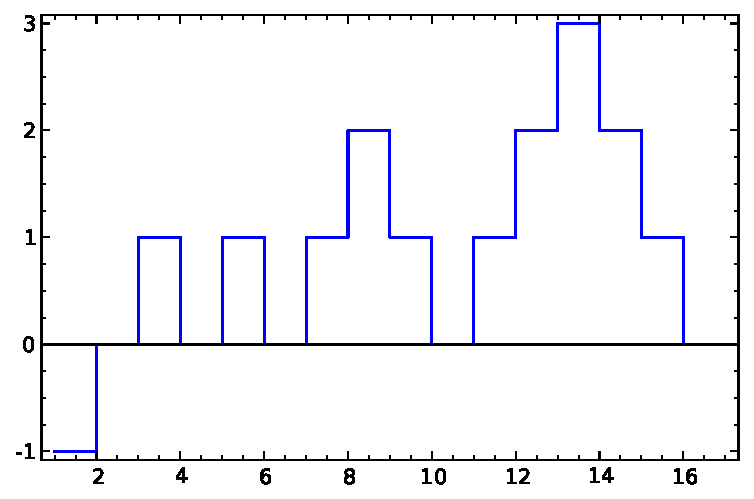
\includegraphics[width=.4\textwidth]{illustrations/liouville-17}
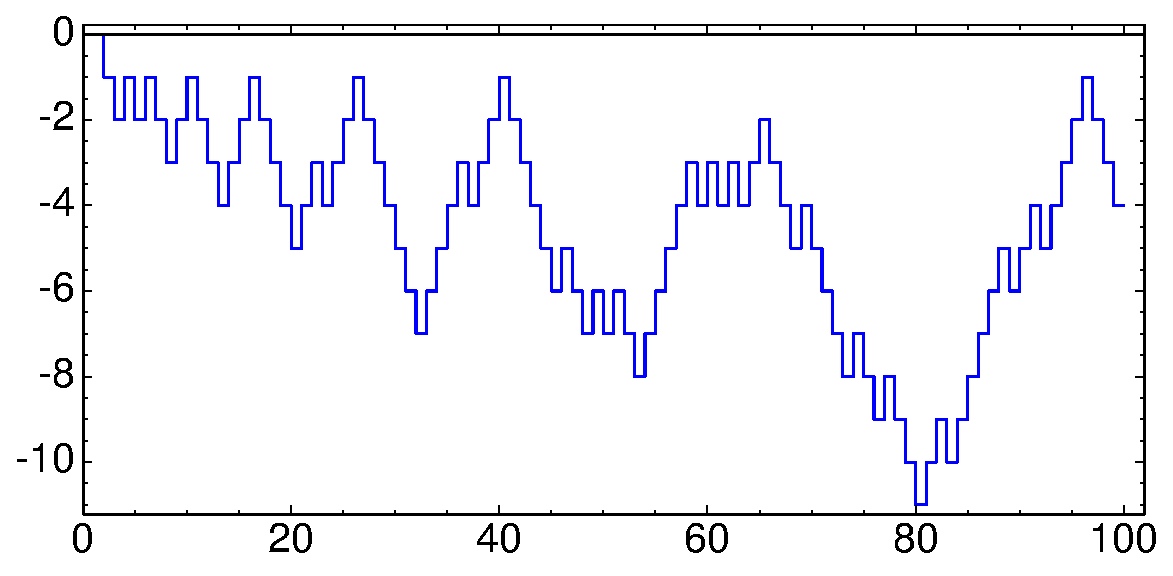
\includegraphics[width=.4\textwidth]{illustrations/liouville-100}\\
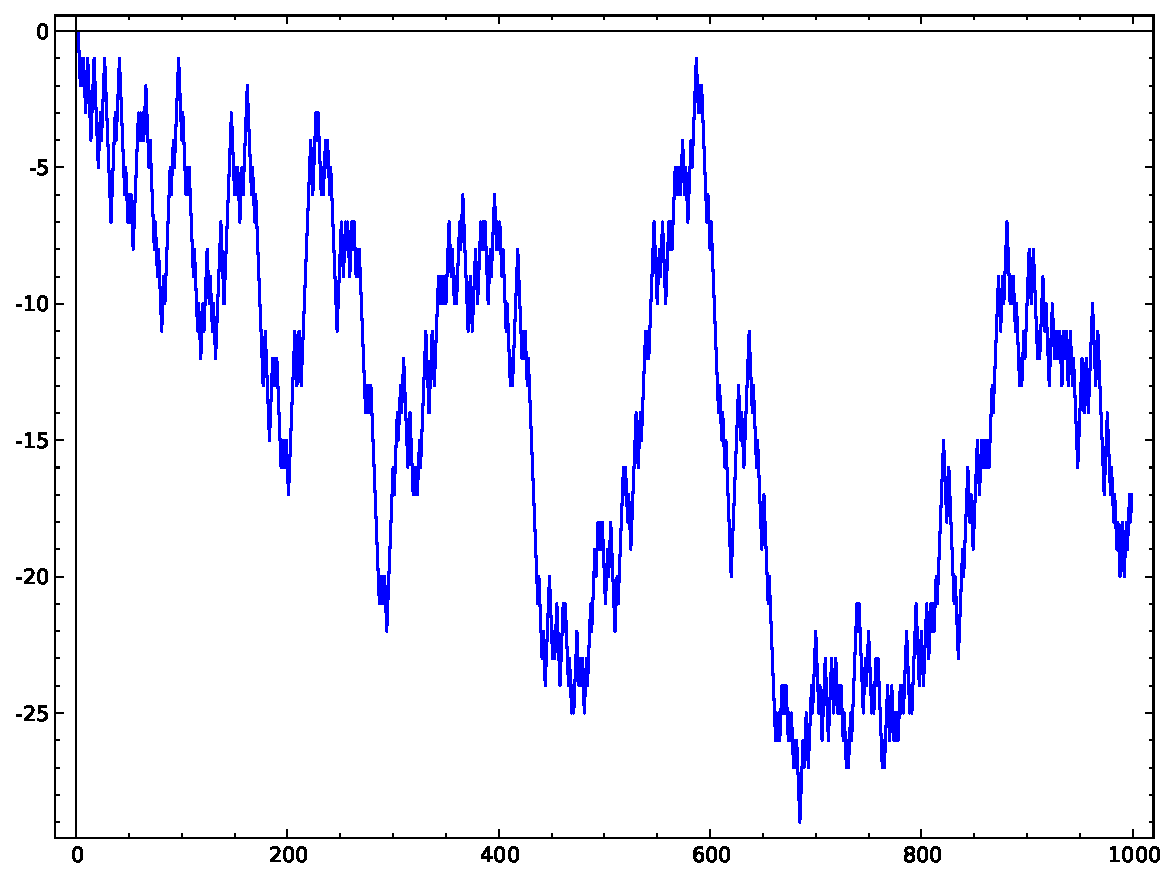
\includegraphics[width=.4\textwidth]{illustrations/liouville-1000}
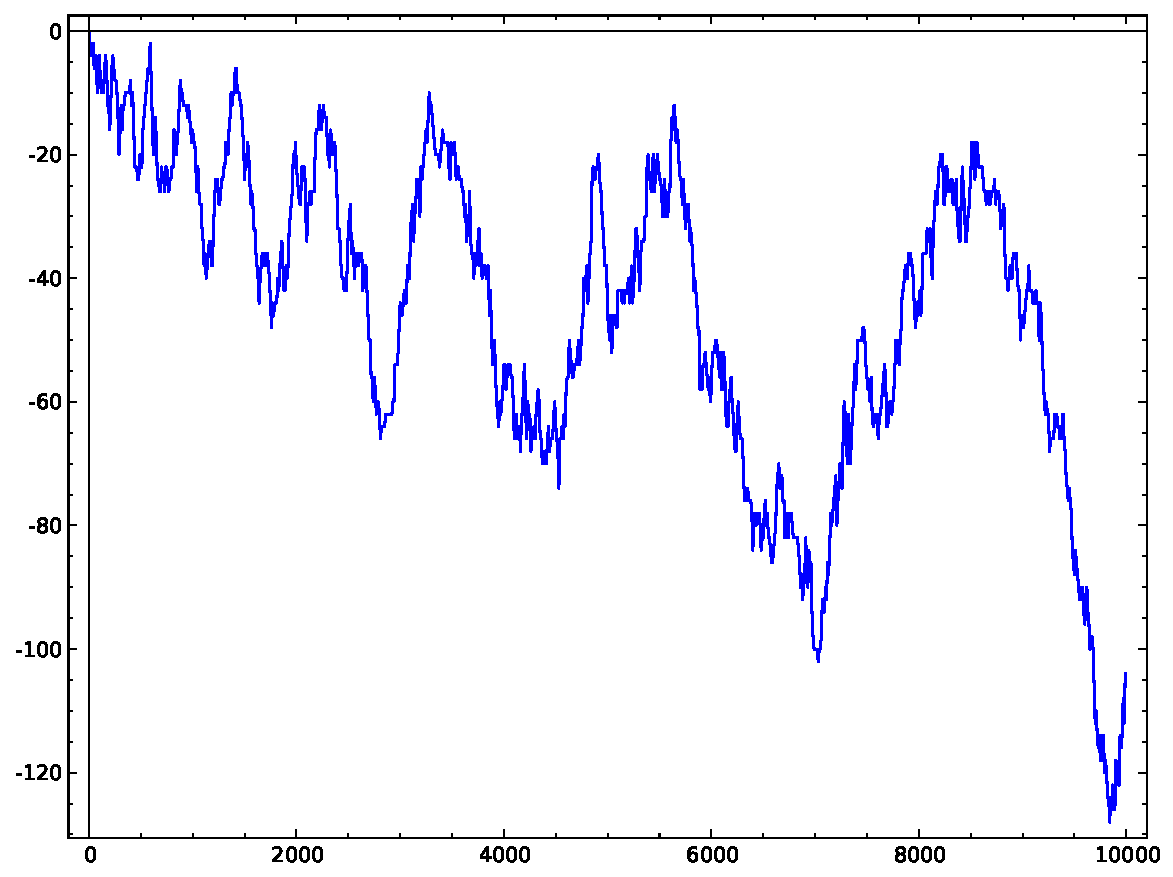
\includegraphics[width=.4\textwidth]{illustrations/liouville-10000}\\
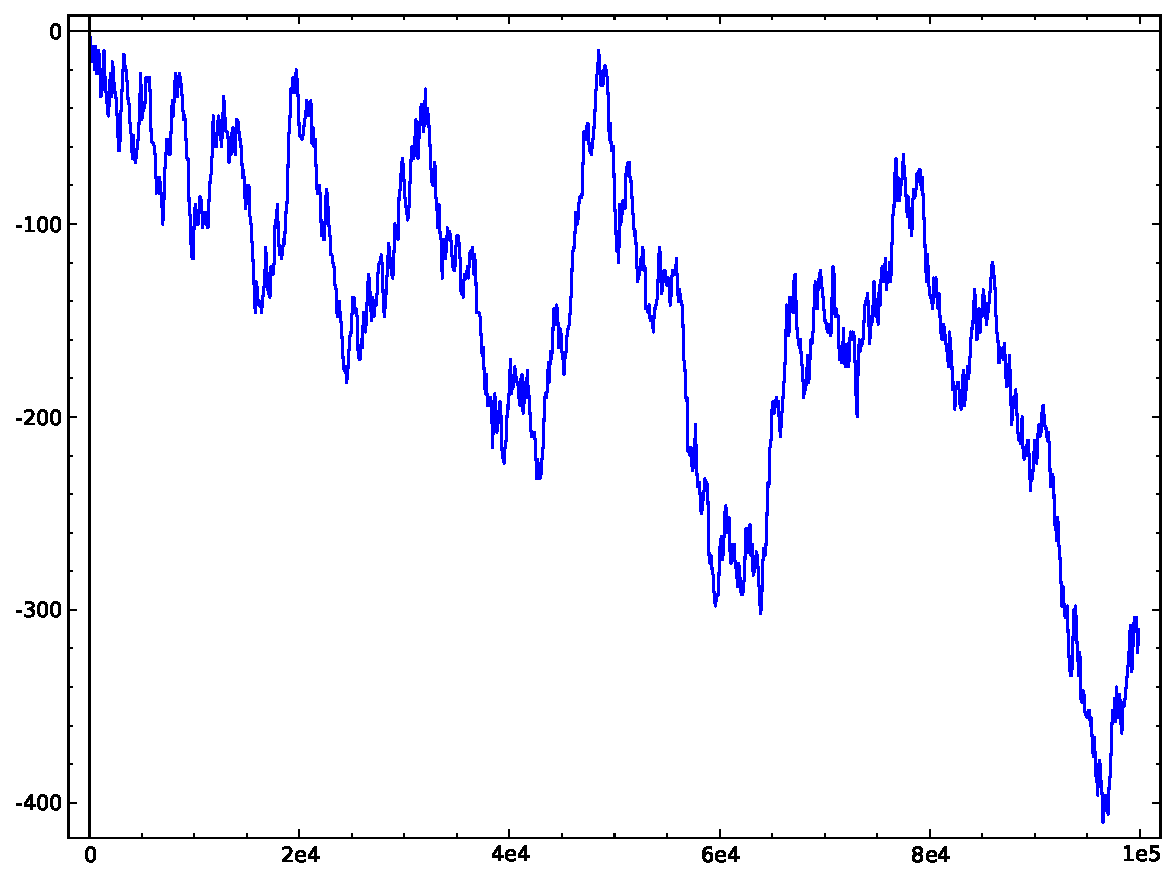
\includegraphics[width=.4\textwidth]{illustrations/liouville-100000}
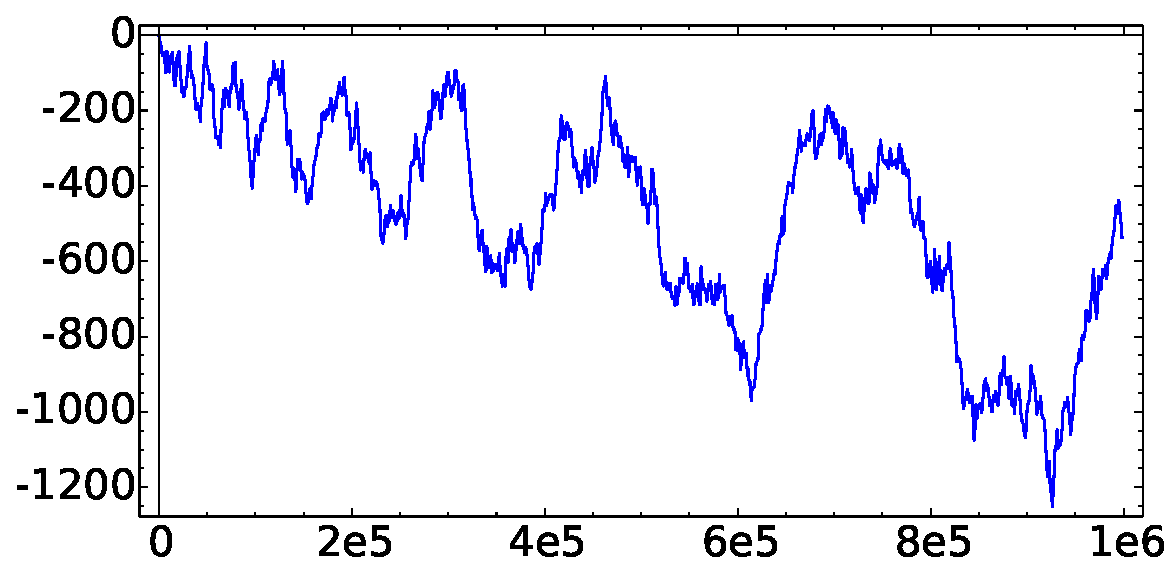
\includegraphics[width=.4\textwidth]{illustrations/liouville-1000000}\\
\caption{Racing Multiplicatively Even and Odd Numbers.\label{fig:liouville}}
\end{figure}

A {\em negative} response to this question---i.e., a proof that any
plot as drawn in Figure~\ref{fig:liouville} never crosses
the $X$-axis---would imply the Riemann Hypothesis!  In contrast to the list of
previous questions, the answer to this question is known (see \bibnote{For more
  details, see P.~Borwein, {\em Sign changes in sums of the Liouville
    Function} and the nice short paper of Norbert Wiener {\em Notes on
    Polya's and Turan's hypothesis concerning Liouville's factor}
  (page 765 of volume II of Wiener's Collected Works); see also:
  G. Polya {\em Vershiedene Bemerkungen zur Zahlentheorie}
  Jahresbericht de Deutschen Mathematiker-Vereinigung, {\bf 28} (1919)
  31--40.}): alas, there is such an $X$.  In 1960, Lehman showed that
for $X=906,400,000$ there are $708$ more multiplicatively even numbers
up to $X$ than multiplicatively odd numbers (Tanaka found in 1980 that
the smallest $X$ such that there are more multiplicative even than odd
numbers is $X=906,150,257$).

%%%%%%%%%%%%%%%%%
%\begin{wrapfigure}{r}{0.2\textwidth}
%    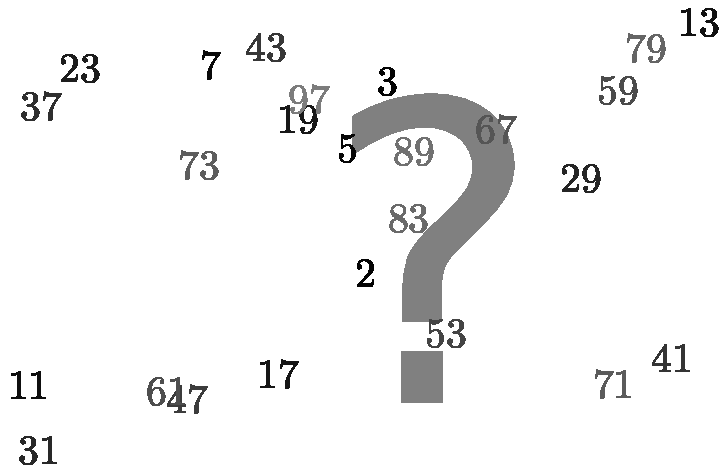
\includegraphics[width=0.2\textwidth]{illustrations/questions}
%\end{wrapfigure}
These are questions that have been asked about primes (and we could
give bushels more as is done in \bibnote{Richard Guy's book {\em Unsolved Problems in Number Theory} (2004).}),
questions expressible in simple vocabulary, that
we can't answer today. We have been studying numbers for over two
millenia and yet we are indeed in the infancy of our understanding.


So we'll continue our discussion by returning to the simplest counting
question about prime numbers.

\chapter{How many primes are there?}

\ill{sieve200}{.8}{Sieving Primes up to 200}

Slow as we are to understand primes, at the very least we can try to
count them. You can see that there are $10$ primes less than $30$, so
you might encapsulate this by saying that the chances that a number
less than $30$ is prime is $1$ in $3$.  This frequency does not
persist, though; here is some more data: There are $25$ primes less
than $100$ (so $1$ in $4$ numbers up to $100$ are prime), there are
$168$ primes less than a thousand (so we might say that among the
numbers less than a thousand the chances that one of them is prime is
roughly $1$ in $6$).

\ill{proportion_primes_100}{1}{Graph of the proportion of primes up to $X$ for each integer $X\leq 100$}

There are 78,498 primes less than a million (so we might say that
the chances that a random choice among the first million numbers is
prime have dropped to roughly $1$ in $13$).

\illtwo{proportion_primes_1000}{proportion_primes_10000}{0.46}{Proportion of primes for $X$ up to $1{,}000$ (left) and $10{,}000$ (right)}

There are 455,052,512 primes less than ten billion; i.e.,
10,000,000,000 (so we might say that the chances are down to roughly
$1$ in $22$).

Primes, then, seem to be thinning out.  We return to the sifting process
we carried out earlier, and take a look at a few graphs, to get a sense of why
that might be so. There are a $100$ numbers less than or equal to
$100$, a thousand numbers less than or equal to $1000$, etc.: the
shaded graph in Figure~\ref{fig:sieve_2_100} that looks like a regular staircase, each step the
same length as each riser, climbing up at, so to speak, a 45 degree
angle, counts all numbers up to and including~$X$.

Following Eratosthenes, we have sifted those numbers, to pan for
primes. Our first move was to throw out roughly half the numbers (the
even ones!) after the number $2$. The cross-hatched bar graph in this
figure which is, with one hiccup, a regular staircase climbing at a
smaller angle, each step twice the lengths of each riser, illustrates
the numbers that are left after one pass through Eratosthenes' sieve,
which includes, of course, all the primes. So, the chances that a
number bigger than $2$ is prime is {\em at most} $1$ in $2$.  Our
second move was to throw out a good bunch of numbers bigger than $3$.
So, the chances that a number bigger than $3$ is prime is going to be
even less.  And so it goes: with each move in our
sieving process we are winnowing the field more extensively, reducing
the chances that the later numbers are prime.

\ill{sieve_2_100}{.8}{Sieving by removing multiples of $2$ up to $100$\label{fig:sieve_2_100}}
\ill{sieve1000}{.8}{Sieving for primes up to $1000$}

The red curve in these figures actually counts the primes: it is the
beguilingly irregular {\em staircase of primes.}  Its height above any
number $X$ on the horizontal line records the number of primes less
than or equal to $X$, the accumulation of primes up to $X$.  Refer to
this number as $\pi(X)$. So $\pi(2)=1$, $\pi(3) = 2$, $\pi(30) = 10$;
of course, we could plot a few more values of $\pi(X)$, like
$\pi(\text{ten billion}) = 455,052,512$.


Let us accompany Eratosthenes for a few further steps in his sieving
process.  Figure~\ref{fig:sieve3_100} contains a graph of all whole
numbers up to 100 after we have removed the even numbers greater than
$2$, and the multiples of $3$ greater than $3$ itself.


\ill{sieves3_100}{.7}{Sieving out multiples of $2$ and $3$.\label{fig:sieve3_100}}


From this graph you can see that if you go ``out a way'' the
likelihood that a number is a prime is less that $1$ in $3
$. Figure~\ref{fig:sieve7_100} contains a graph of what Eratosthenes
sieve looks like up to 100 after sifting $2,3,5,$ and $7$.



\ill{sieves7_100}{.7}{Sieving out multiples of $2$, $3$, $5$, and $7$.\label{fig:sieve7_100}}


This data may begin to suggest to you that as you go further and
further out on the number line the percentage of prime numbers among
all whole numbers tends towards $0\%$ (it does).


To get a sense of how the primes accumulate, we will take a look at
the staircase of primes for $X= 25$ and $X=100$ in Figures~\ref{fig:staircase25}
and \ref{fig:staircase100a}.

\ill{prime_pi_25_aspect1}{.8}{Staircase of primes up to 25\label{fig:staircase25}}
\ill{prime_pi_100_aspect1}{.8}{Staircase of primes up to 100\label{fig:staircase100a}}



\chapter{Prime numbers viewed from a distance}
The striking thing about these figures is that as the numbers get
large enough, the jagged accumulation of primes, those
quintessentially discrete entities, becomes smoother and smoother, to
the eye. How strange and wonderful to watch, as our viewpoint zooms
out to larger ranges of numbers, the accumulation of primes taking on
such a smooth and elegant shape.

\illtwo{prime_pi_1000}{prime_pi_10000}{0.4}{Staircases of primes up to 1,000 and 10,000\label{fig:staircases2}}

\ill{prime_pi_100000}{.8}{Primes up to 100,000\label{fig:pn100000}.
Note that the axis label ``6e4'' means $6 \times 10^4$.}



But don't be fooled by the seemingly smooth shape of the curve in the
last figure above: it is just as faithful a reproduction of the
staircase of primes as the typographer's art can render, for there are
thousands of tiny steps and risers in this curve, all hidden by the
thickness of the print of the drawn curve in the figure.  It is
already something of a miracle that we can approximately describe the
build-up of primes, somehow, using a {\em smooth curve}.  But {\em
  what} smooth curve?


That last question is {\em not} rhetorical. If I draw a curve with
chalk on the blackboard, this can signify a myriad of smooth
(mathematical) curves all encompassed within the thickness of the
chalk-line, all--if you wish--reasonable approximations of one
another. So, there are many smooth curves that fit the chalk-curve.
With this warning, but very much fortified by the data of Figure~\ref{fig:pn100000},
let us ask: {\em what is a smooth curve that is a reasonable
  approximation to the staircase of primes?}

\chapter{Pure and applied  mathematics}\label{ch:pureapplied}

Mathematicians seems to agree that, loosely speaking, there are two
types of mathematics: {\em pure} and {\em applied}. Usually---when we
judge whether a piece of mathematics is pure or applied---this
distinction turns on whether or not the math has application to the
``outside world,'' i.e., that {\em world} where bridges are built,
where economic models are fashioned, where computers churn away on the
Internet (for only then do we unabashedly call it {\em applied math}),
or whether the piece of mathematics will find an important place
within the context of mathematical theory (and then we label it {\em
  pure}).  Of course, there is a great overlap (as we will see later,
Fourier analysis plays a major role both in data compression and in
pure mathematics).

 Moreover, many questions in
mathematics are ``hustlers'' in the sense that, at first view, what is
being requested is that some simple task be done (e.g., the question
raised in this book, {\em to find a smooth curve that is a reasonable
  approximation to the staircase of primes}).  And only as things
develop is it discovered that there are payoffs in many unexpected
directions, some of these payoffs being genuinely applied (i.e., to
the practical world), some of these payoffs being pure (allowing us
to strike behind the mask of the mere appearance of the mathematical
situation, and get at the hidden fundamentals that actually govern the
phenomena), and some of these payoffs defying such simple
classification, insofar as they provide powerful techniques in other
branches of mathematics.  The \RH{}---even in its current
unsolved state---has already shown itself to have all three types of
payoff.

The particular issue before us is, in our opinion, twofold, both
applied, and pure: can we curve-fit the ``staircase of primes'' by a
well approximating smooth curve given by a simple analytic formula?
The story behind this alone is
marvelous, has a cornucopia of applications, and we will be telling it
below. But our curiosity here is driven by a question that is pure,
and less amenable to precise formulation: are there mathematical
concepts at the root of, and more basic than (and ``prior to,'' to
borrow Aristotle's use of the phrase,) {\em prime numbers}--concepts
that account for the apparent complexity of the nature of primes?


\chapter{A probabilistic ``first'' guess\label{sec:firstguess} }

\ill{gauss}{.3}{Gauss}

The search for such approximating curves began, in fact, two centuries
ago when Carl Friedrich Gauss defined a certain beautiful curve that,
experimentally, seemed to be an exceptionally good fit for the
staircase of primes.

\ill{pi_Li}{.7}{Plot of $\pi(X)$ and Gauss's smooth curve $G(X)$}

Let us denote Gauss's curve $G(X)$; it has an
elegant simple formula comprehensible to anyone who has had a tiny bit
of calculus.  If you make believe that the chances that a number $X$ is
a prime is inversely proportional to the number of digits of $X$ you
might well hit upon Gauss's curve.
That is,
\vskip10pt
$$G(X)\hskip40pt  {\rm is\ roughly\ proportional\ to} \hskip40pt  {\frac{X}{{\rm the\ number\ of\ digits\ of\ } X}}.$$
\vskip10pt
But to describe Gauss's guess precisely we need to discuss the {\it natural logarithm} ``$\log(X)$'' which is an elegant smooth function of real numbers $X$ that is roughly proportional to the number of digits of the whole number part of $X$.



\ill{log}{.8}{Plot of the natural logarithm $\log(X)$}


 Euler's famous constant $e=2.71828182\ldots$, which is the limit
 of the sequence
 $$\left(1+{\frac{1}{2}}\right)^2,
       \left(1+{\frac{1}{3}}\right)^3,
       \left(1+{\frac{1}{4}}\right)^4, \dots,$$
is used in the definition of $\log$:
\begin{center}
{\em $A = \log(X)$ is the number $A$ for which $e^A = X$.}
\end{center}
Before electronic calculators, logarithms were frequently used to
speed up calculations, since logarithms translate difficult multiplication
problems into easier addition problems which can be done mechanically.
Such calculations use that the logarithm of a product is the sum of the logarithms
of the factors; that is, $$\log(X\cdot Y) = \log(X) + \log(Y).$$
%FROM -- YURI TSCHINKEL's: ''ABOUT THE COVER: ON THE DISTRIBUTION OF PRIMESÑGAUSSÕ TABLES ''

% From: http://en.wikipedia.org/wiki/File:Slide_rule_scales_back.jpg
\ill{slide_rule}{.8}{A slide rule  computes $2X$ by using that $\log(2X)=\log(2)+\log(X)$\label{fig:slide_rule}}

In Figure~\ref{fig:slide_rule} the numbers printed (on each of the slidable pieces of the rule)
are spaced according to their logarithms, so that when one slides the
rule arranging it so that the printed  number $X$ on one piece lines up
with the printed number $1$ on the other, we get that for every number $Y$
printed on the first piece, the printed number on the other piece that
is  aligned with it is the product $XY$; in effect the ``slide'' adds
$\log(X)$ to $\log(Y)$ giving $\log(XY)$.

% I found this here: http://kr.blog.yahoo.com/kimxx168/498
% It is referenced in http://www.ams.org/bull/2006-43-01/S0273-0979-05-01096-7/home.html
% but that link is broken.
\ill{gauss_tables_half}{.9}{A Letter of Gauss\label{fig:gauss_letter}}

In 1791, when Gauss was 14 years old, he received a book that contained
logarithms of numbers up to $7$ digits and a table of primes up to 10,009.
Years later, in a letter
written in 1849 (see Figure~\ref{fig:gauss_letter}), Gauss
claimed that as early as 1792 or 1793 he had already observed that the
density of prime numbers over intervals of numbers of a given rough
magnitude $X$ seemed to average $1/\log(X)$.

 Very {\em very} roughly speaking, this
means that {\em the number of primes up to $X$ is approximately $X$ divided by
twice the number of digits of $X$}.  For example,
the number of primes less than $99$ should be roughly
$$
   \frac{99}{2\times 2} = 24.75 \approx  25,
$$
which is pretty amazing, since the correct number of
primes up to $99$ is $25$.  The number of primes up to $999$ should
be roughly
$$
   \frac{999}{2\times 3} = 166.5 \approx  167,
$$
which is again close, since there are 168 primes up to $1000$.
The number of primes up to $999{,}999$ should be roughly
$$
   \frac{999999}{2\times 6} = 83333.25 \approx  83{,}333,
$$
which is close to the correct count of $78{,}498$.

Gauss guessed that the expected number of primes up to $X$
is approximated by the area under the
graph of $1/\log(X)$ from $2$ to $X$ (see Figure~\ref{fig:G}).
The area under $1/\log(X)$ up to $X=999{,}999$ is $78{,}626.43\ldots$, which
is remarkably close to the correct count $78{,}498$ of the primes
up to $999{,}999$.

\illthree{area_under_log_graph_30}{area_under_log_graph_100}{area_under_log_graph_1000}{.27}{The
  expected tally of the number of primes $\leq X$ is approximated by the
  area underneath the graph of $1/\log(X)$ from $1$ to $X$.\label{fig:G}}


Gauss was an inveterate computer:
he wrote in his 1849 letter  that
there are $216{,}745$ prime numbers less than three million (This is
wrong: the actual number of these primes is $216{,}816$). Gauss's curve $G(X)$
predicted that there would be $216{,}970$ primes---a miss, Gauss
thought, by
$$225 = 216{,}970 - 216{,}745$$
(but actually he was closer than he thought: the
prediction of the curve $G(X)$ missed by a mere $154 = 216{,}970  - 216{,}816$)
%; not as close as the 2004 US
%elections, but pretty close nevertheless).
Gauss's computation brings up two queries: will this spectacular ``good
fit'' continue for arbitrarily large numbers? and, the (evidently
prior) question: what counts as a good fit?



\chapter{What is a ``good approximation''?}\label{sec:sqrterror}

If you are trying to estimate a number, say, around ten thousand, and
you get it right to within a hundred, let us celebrate this kind of
accuracy by saying that you have made an approximation with {\em
  square-root error} (${\sqrt{10{,}000}}=100$). Of course, we should
really use the more clumsy phrase ``an approximation with at worst
{\em square-root error.}''  Sometimes we'll simply refer to such
approximations as {\em good approximations.} If you are trying to
estimate a number in the millions, and you get it right to within a
thousand, let's agree that---again---you have made an approximation
with {\em square-root error} (${\sqrt{1{,}000{,}000}}=1{,}000$).
Again, for short, call this a {\em good approximation.} So, when Gauss
thought his curve missed by $226$ in estimating the number of primes
less than three million, it was well within the margin we have given
for a ``good approximation.''
\bibnote{If $f(x)$ and
$g(x)$ are real-valued functions of a real variable $x$ such that
for any
$\epsilon >0$ both of them take their values between $ x^{1-\epsilon}$
and $ x^{1+\epsilon}$ for
$x$
sufficiently large, then say that $f(x)$ and $g(x)$ are {\bf good
approximations of one another} if,
for any positive $\epsilon$ the absolute values of their difference
is less than $ x^{{1\over
2}+\epsilon}$ for
$x$
sufficiently large. The functions $\Li(X)$ and $R(X)$ of are good approximations of
one another.}

More generally, if you are trying to estimate a number that has $D$
digits and you get it almost right, but with an error that has no more
than, roughly, half that many digits, let us say, again, that you have
made an approximation with {\em square-root error} or synonymously, a
{\em good approximation}.


This rough account almost suffices for what we will be discussing
below, but to be more precise, the specific {\em gauge of accuracy}
that will be important to us is not for a mere {\em single} estimate
of a {\em single} error term,

 \centerline{Error term\ \  =\ \    Exact Value\ \   -\ \   Our ``good  approximation''}



 \noindent but rather for {\em infinite sequences} of estimates of
 error terms. Generally, if you are interested in a numerical quantity
 $q(X)$ that depends on the real number parameter $X$ (e.g., $q(X)$
 could be $\pi(X)$, ``the number of primes $< X$'') and if you have an
 explicit candidate ``approximation,'' $q_{\rm approx}(X)$, to this
 quantity, let us say that $q_{\rm approx}(X)$ is {\bf essentially a
   square-root accurate approximation to $q(X)$} if for {\em any}
 given exponent greater than $0.5$ (you choose it: $0.501$, $0.5001$,
 $0.50001$, $\dots$ for example) and for large enough $X$---where the
 phrase ``large enough'' depends on your choice of exponent---the {\bf
   error term}---i.e., the difference between $q_{\rm approx}(X)$ and
 the {\em true} quantity, $q(X)$, is, in absolute value, less than
 $q_{\rm approx}(X)$ raised to that exponent (e.g. $< X^{0.501}$, $<
 X^{0.5001}$, etc.). Readers who know calculus and wish to have a
 technical formulation of this definition of {\em good approximation}
 might turn to the endnote $^2$ for a precise statement.
If you found the above confusing, don't worry: again, a
square-root accurate approximation is one in which at least roughly
half the digits are correct.


\begin{remark}
  To get a feel for how basic the notion of {\em approximation to data
    being square root close to the true values of the data} is---and
  how it represents the ``gold standard'' of accuracy for
  approximations, consider this fable.

  Imagine that the devil had the idea of saddling a large committee of
  people with the task of finding values of $\pi(X)$ for various large
  numbers $X$.  This he did in the following manner, having already
  worked out which numbers are prime himself. Since the devil is, as
  everyone knows, {\em into the details,} he has made no mistakes: his
  work is entirely correct.  He gives each committee member a copy of
  the list of all {\em prime numbers} between $1$ and one of the large
  numbers $X$ in which he was interested.  Now each committee member
  would count the number of primes by doing nothing more than
  considering each number, in turn, on their list and tallying them
  up, much like a canvasser counting votes; the committee members  needn't even know that these numbers are prime, they just think of these numbers as items on their list. But since they are human,
  they will indeed be making mistakes, say $0.001\%$ of the time.
  Assume further that it is just as likely for them to make the
  mistake of undercounting or overcounting.  If many people are
  engaged in such pursuit, some of them might over-count $\pi(X)$;
  some of them might under-count it. The average error (over-counted
  or undercounted) would be proportional to~${\sqrt X}$.

  In the next chapter we'll view these under-counts and over-counts as analogous to a random walk.


\end{remark}


\chapter{Square Root Error and Random Walks}

 To take a random walk along a (straight) East-West path  you would start at your home base, but every minute, say, take a step along the path, each step being of the same length, but randomly either East or West. After $X$ minutes, how far are you from your home base?

  The answer to this {\it cannot} be a specific number, precisely because you're making a random decision that affects that number for each of the $X$ minutes of your journey. It is more reasonable to ask a statistical version of that question. Namely, if you took {\it many} random walks $X$ minutes long, then---on the average---how far would you be from your home base?  The answer, as is illustrated by the figures below, is that the average distance you will find yourself from home base after (sufficiently many of) these excursion is proportional to ${\sqrt X}$. (In fact, the average is equal to $\sqrt{\frac{2}{\pi}}\cdot {\sqrt X}$.)

  To connect this with the committee members' histories of errors, described in the fable in Chapter~\ref{sec:sqrterror}, imagine  every  error (under-count or over-count by $1$) the committee member makes, as a `step' East for under-count and West for over-count. Then if such errors were made, at a constant frequency over the duration of time spent counting, and if the over- and under-counts were equally likely and random, then one can model the committee members' computational  accuracy by a random walk. It would be---in the terminology we have already discussed---no better than {\it square-root accurate}; it would be subject to {\it square-root error}.

   To get a real sense of how constrained random walks are by this `square-root law,' here are a few numerical experiments of random walks. The left-hand squiggly (blue) graphs in Figures~\ref{fig:random_walks_3}--\ref{fig:random_walks_1000} below are computer-obtained random walk trials (three, ten, a hundred, and a thousand random walks). The blue curve in the right-hand graphs of those four figures is the average distance from home-base of the corresponding (three, ten, a hundred, and a thousand) random walks.
The red curve in each figure below is the graph of the quantity $\sqrt{\frac{2}{\pi}}\cdot {\sqrt X}$ over the $X$-axis.
As the number of random walks increases, the red curve
better and better approximates the average distance.

\illtwo{random_walks-3}{random_walks-3-mean}{.45}{Three Random Walks\label{fig:random_walks_3}}

\illtwo{random_walks-10}{random_walks-10-mean}{.45}{Ten Random Walks\label{fig:random_walks_10}}

\illtwo{random_walks-100}{random_walks-100-mean}{.45}{One Hundred Random Walks\label{fig:random_walks_100}}

\illtwo{random_walks-1000}{random_walks-1000-mean}{.45}{One Thousand Random Walks\label{fig:random_walks_1000}}





\chapter[What is Riemann's Hypothesis?] { What is Riemann's Hypothesis?  ({\em first formulation})\label{sec:rh1}}



Recall from Chapter~\ref{sec:firstguess} that a rough guess for an approximation to
$\pi(X)$, the number of primes $< X$, is given by the function
$X/\log(X)$. Recall, as well, that a refinement of that guess, offered by Gauss, stems from this curious thought:  the `probability' that a number $N$ is a prime  is proportional to the reciprocal of its number of digits; more precisely the probability is $1/\log(N)$.  This would lead us to  guess that the approximate value of $\pi(X)$ would be
the area of the region from $2$ to $X$ under the graph of
$1/\log(X)$, a quantity sometimes referred to as $\Li(X)$.
``Li'' (pronounced L$\overline{\rm i}$) is short for {\em logarithmic integral},
because the area of the region from $2$ to $X$ under $1/\log(X)$
is the {\em integral} $\int_2^t 1/\log(X) dt$.




Figure~\ref{fig:threeplots} contains a graph of the three functions
$\Li(X)$, $\pi(X)$, and $X/\log X$ for $X\leq 200$.
But data, no matter how impressive, may be deceiving (as we learned in
Chapter~\ref{ch:further}). If you think
that  the three graphs  never cross for all large values of $X$,  and
that we have the simple relationship  $X/\log(X) < \pi(X) < \Li(X)$ for
large $X$, turn to this endnote.
\bibnote{See \url{http://en.wikipedia.org/wiki/Skewes'_number}.}


\ill{three_plots}{.9}{Plots of $\Li(X)$ (top), $\pi(X)$ (in the middle), and $X/\log(X)$ (bottom).\label{fig:threeplots}}

Let $X=10^{24}$.  Then \label{pili_vals} (see \bibnote{This computation of $\pi(X)$ was done by David J. Platt in 2012,
and is the largest value of $\pi(X)$ ever computed.  See
\url{http://arxiv.org/abs/1203.5712} for more details.})
\begin{align*}
  \pi(X) &= 18{,}435{,}599{,}767{,}349{,}200{,}867{,}866\\
  \Li(X) &= 18{,}435{,}599{,}767{,}366{,}347{,}775{,}143.10580\ldots \\
  X/(\log(X)-1)  &=
            18{,}429{,}088{,}896{,}563{,}917{,}716{,}962.93869\ldots\\
  \Li(X) - \pi(X) &= \hspace{7em}
     17{,}146{,}907{,}277.105803\ldots\\
  \sqrt{X}\cdot \log(X) &= \hspace{5.2em}
     55{,}262{,}042{,}231{,}857.096416 \ldots
\end{align*}



More fancifully, we can think of the error in this approximation to $\pi(X)$, i.e., $|\Li(X)-\pi(X)|$, (the absolute value) of the difference between $\Li(X)$ and $\pi(X)$, as (approximately) the result of  a walk having roughly $X$ steps where you move by the following rule:  go  east by a distance of $1/\log N$ feet if $N$ is not a prime and west by a distance of $1-\frac{1}{\log N}$ feet if $N$ is a prime. Your distance, then, from home base after $X$ steps is approximately $|\Li(X)-\pi(X)|$.

We have no idea if this picture of things resembles a truly {\it random walk} but at least it makes it reasonable to ask the question: is $\Li(X)$  {\it essentially a square root approximation} to
$\pi(X)$? Our first formulation of Riemann's
Hypothesis, says yes:

      \begin{center}
       \shadowbox{ \begin{minipage}{0.9\textwidth}
\mbox{}       \vspace{0.2ex}
       \begin{center}{\bf\large The {\bf \RH{}} (first formulation)}\end{center}
       \medskip

For any real number $X$ the number of prime numbers less than $X$ is
approximately $\Li(X)$ and this approximation is essentially square
root accurate. See \bibnote{In fact, the Riemann Hypothesis is equivalent to $|\Li(X) - \pi(X)| \leq \sqrt{X}\log(X)$ for all $X\geq 2.01$.  See Section 1.4.1 of Crandall-Pomerance's book {\em Prime numbers,
a computational perspective}.}.
\label{rh:first}

\vspace{1ex}
\end{minipage}}
      \end{center}

\chapter{The mystery moves to  the error term}

 Let's think of what happens when you have a {\it mysterious quantity} (say,  a function of a real number $X$) you wish to understand. Suppose you manage to approximate that quantity by  an easy to understand  expression---which we'll call the  ``dominant term,"--- that is also simple to compute, but only approximates your mysterious quantity. The approximation is not exact; it has a possible error, that happily is significantly smaller than the size of the dominant term. `Dominant,' here just means exactly that: it  is of size significantly larger than the error of approximation.

 $${\it Mysterious\  quantity}(X)\ \ = \ \ {\it Simple, \ but \ dominant\ quantity}(X) \ + \ {\it Error}(X).$$

 If all you are after is a general estimate of {\it size}  your job is done. You might declare victory and ignore ${\it Error}(X)$ as being---in size--negligible. But if you are interested in the deep structure of your {\it mysterious quantity} perhaps all you have done is to manage to transport most questions about it to  ${\it Error}(X)$. In conclusion, ${\it Error}(X)$ is now your new mysterious quantity.

 Returning to the issue of $\pi(X)$ (our {\it mysterious quantity}) and $Li(X)$ (our {\it dominant term}) the first formulation of the Riemann Hypothesis  (as in Chapter \ref{sec:rh1} above)  puts the spotlight on the {\it Error\ term}, $|\Li(X) - \pi(X)|$ which therefore deserves our scrutiny, since---after all---we're not interested in merely counting the primes: we want to understand as much as we can of their structure.

   To get a feel for this error term, we shall smooth it out a bit, and look at a few of its graphs.


\chapter {C{\'e}saro Smoothing}\label{ces}

Often when you hop in a car and reset the trip counter, the car
will display information about your trip.  For instance, it might show you the
average speed up until now during your trip; this number
is ``sticky'', changing much less erratically than your
actual speed, and you might use it to make a rough estimate of
how long until you will reach your destination.
Your car is computing the {\em C{\'e}saro smoothing }of your speed.
We can use this same idea to better understand the behavior
of other things, such as the sums appearing in
the previous chapter.
\ill{camaro}{.7}{A 2013 Camaro SS Dashboard}
%I took this picture of my rental car -- William Stein.

 Suppose you are trying to say something intelligent about the behavior of a certain quantity that varies with time in what seems to be a somewhat erratic, volatile pattern. Call the quantity $f(t)$ and think of it as a function defined for positive real values of `time' $t$.  The first natural impulse might be to take some sort of `average value' of  $f(t)$ overt a time interval, say fro $0$ to $T${\footnote{ For readers who know calculus: that  average would be ${\frac{1}{T}}\int_0^Tf(t)dt$.}.   This would indeed be an intelligent thing to do if this average stabilized and depended relatively little on  the interval of time over which one is computing this average, e.g., if that interval were large enough.  Sometimes, of course, these averages themselves are relatively sensitive to the times $T$ that are chosen, and don't stabilize. In such a case, it usually pays to consider {\it all} these averages  as  your chosen $T$ varies, as a function (of $T$) in its own right{\footnote{ For readers who know calculus: this is
  $$F(T):= {\frac{1}{T}}\int_0^Tf(t)dt.$$}.
   This new function $F(T)$, called the {\bf C{\'e}saro Smoothing} of the function $f(t)$, is a good indicator of certain eventual trends of the original function $f(t)$ that is less visible directly from the function $f(t)$.  The effect of passing from $f(t)$ to $F(T)$ is to `smooth out' some of the volatile local behavior of the original function, as can be seen in the figure below.


\ill{cesaro}{.8}{The red plot is the C{\'e}saro smoothing of the blue plot}
\chapter{ A view of $|\Li(X) - \pi(X)|$}
 Returning to our mysterious error term,  consider Figure \ref{fig:li-minus-pi-250000} where the volatile blue curve is $|\Li(X) - \pi(X)|$, its C{\'e}saro smoothing is the red relatively smooth curve, and the blue curve is the graph of $\sqrt{\frac{2}{\pi}}\cdot \sqrt{x/\log(x)}$ over the range of $X\le 250,00$.

\ill{li-minus-pi-250000}{.9}{$\Li(x)-\pi(x)$ (blue middle), its C{\'e}saro smoothing (red bottom), and
$\sqrt{\frac{2}{\pi}}\cdot \sqrt{x/\log(x)}$ (top), all for $x\leq 250{,}000$\label{fig:li-minus-pi-250000}}

% TODO: this is from http://seriesdivergentes.wordpress.com/2011/07/21/john-e-littlewood/
\begin{wrapfigure}{r}{0.23\textwidth}
    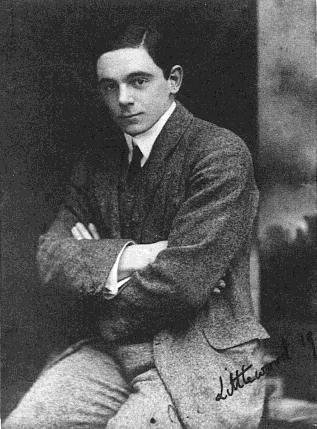
\includegraphics[width=0.23\textwidth]{illustrations/littlewood}\\
    Littlewood
\end{wrapfigure}
Data such as this graph can be revealing and misleading at the same time.  The blue volatile graph ($\Li(x)-\pi(x)$) {\it seems} to be sandwiched between two rising functions, but this will not continue for all values of $x$.  The Cambridge University mathematician, John Edensor Littlewood, proved in 1914 that there {\it exists} a real number $x$ for which the quantity $\Li(x)-\pi(x)$ vanishes and crosses over into negative values.  This theorem attracted lots of attention at the time (and continues to do so) because of the inaccessibility of achieving good estimates (upper or lower bounds) for the first such number.  That `first' $x$ for which   $\Li(x) =\pi(x)$ is called {\bf Skewes Number} in honor of the South African mathematician (a student of Littlewood)  Stanley Skewes, who (in 1933) gave the  first---fearfully large----upper bound for that number (conditional on RH!).  Despite a steady stream of subsequent improvements, we currently can only  locate Skewes Number  as being in the range:

$$
10^{14}\ \ \ \le\ \ \ {\rm Skewes\ Number}\ \ \ <\ \ \    10^{317},
$$ and it is proven that at some  values of $x$ fairly close to the upper bound $10^{317}$   $\pi(x)$ is greater than $\Li(x)$. So  the trend suggested in Figure \ref{fig:li-minus-pi-250000} will not continue indefinitely.






\chapter{The Prime Number Theorem\label{sec:pnt}}

Take a look at Figure~\ref{fig:threeplots} again.  All three functions, $X/\log(X)$,
$\Li(X)$ and $\pi(X)$ are ``going to infinity with $X$'' (this means
that for any real number $R$, if $X$ is taken to be sufficiently
large, the values of these functions at $X$ will exceed $R$).

Are these functions ``going to infinity'' at {\it the same rate}?

To answer such a question, we have to know what we mean by {\it going
  to infinity at the same rate}. So, here's a definition. Two
functions, $A(X)$ and $B(X)$, that each go to infinity will be said to
{\bf go to infinity at the same rate} if their {\it ratio}
$$A(X)/B(X)$$
tends to $1$ as $X$ goes to infinity.

If for example  two functions, $A(X)$ and $B(X)$ that take positive whole number values, have the same number of digits for large $X$  and if,  for any
number you give us, say: a million (or a billion, or a trillion) and if $X$ is large enough, then the
``leftmost'' million (or billion, or trillion) digits of $A(X)$ and $B(X)$ are the same,  then  $A(X)$ and $B(X)$  {\it go to infinity at the same rate}.


While we're defining things, let us say that two functions, $A(X)$
and $B(X)$, that each go to infinity {\bf go to infinity at
similar rates} if there are two positive constants $c$ and $C$
such that for $X$ sufficiently large the {\it ratio}
$$
      A(X)/B(X)
$$
is greater than $c$ and smaller than $C$.

    \ill{similar_rates}{1.0}{The polynomials $A(X)=2 X^{2} + 3 X - 5$ (bottom)
and $B(X)=  3 X^{2} - 2 X + 1$ (top) go to infinity at similar rates.\label{fig:simrates}}



For example, two polynomials in $X$ with positive leading coefficient
{\it go to infinity at the same rate} if and only if they have the
same degrees and the same leading coefficient; they {\it go to
  infinity at similar rates} if they have the same degree.
See Figure~\ref{fig:simrates}. %where we may take $c=1/2$ and $C=1$.

 \ill{same_rates}{1.0}{The polynomials $A(X)=X^{2} + 3 X - 5$ (top)
and $B(X)= X^{2} - 2 X + 1$ (bottom) go to infinity
at the same rate.\label{fig:samerate}}



Now a theorem from elementary calculus tells us that the ratio of
$\Li(X)$ to $X/\log(X)$ tends to $1$ as $X$ gets larger and larger.
That is---using the definition we've just introduced--- $\Li(X)$ and
$X/\log(X)$ go to infinity at the same rate (see
\bibnote{For a proof of this here's a hint. Compute the difference
between the derivatives of $\Li(x)$ and of  $x/\log x$. The answer
is $1/\log^2(x)$.  So you must show that the ratio of
$\int_2^X dx/\log^2(x)$ to $\Li(x)= \int_2^Xdx/\log(x)$
tends to zero as~$x$ goes to infinity, and this is a good
Calculus exercise.})


Recall (on page 10 above)  that
if $X = 10^{23}$, the top eleven digits of $\pi(X)$ and $\Li(X)$ are the same: $19253203916.$ Well, that's a good start. Can we guarantee that for  $X$ large enough, the ``top'' million (or billion, or trillion) digits of $\pi(X)$ and $\Li(X)$ are the same? I.e., that these two functions go to infinity at the same rate?

The \RH{}, as we have just formulated it, would tell us
that the {\it difference} between $\Li(X)$ and $\pi(X)$ is pretty small
in comparison with the size of $X$. This information would imply (but
would be {\it much} more precise information than) the statement that
the {\it ratio} $\Li(X)/\pi(X)$ tends to $1$, i.e., that $\Li(X)$ and
$\pi(X)$ go to infinity at the same rate.

This last statement gives, of course, a far less precise relationship
between $\Li(X)$ and $\pi(X)$ than the \RH{} (once it is proved!)
would give us.  The advantage, though, of the less precise statement
is that it is currently known to be true, and---in fact---has been
known for over a century. It goes under the name of


 \noindent {\bf The Prime Number Theorem:\ \ } $\Li(X)$ and $\pi(X)$ go to infinity at the same rate.


   Since $\Li(X)$ and $X/\log(X)$ go to infinity at the same rate, we could
   equally well have expressed the ``same'' theorem by saying:


  \noindent {\bf The Prime Number Theorem:\ \ } $X/\log(X)$ and $\pi(X)$ go to infinity at the same rate.


   This fact is a very hard-won piece of mathematics!  It was proved
   in 1896 independently by Hadamard and de la Vall\'{e}e Poussin.


   A milestone in the history leading up to the proof of Prime Number
   Theorem is the earlier work of Chebyshev (see
   \url{http://en.wikipedia.org/wiki/Chebyshev_function}) showing that
   (to use the terminology we introduced) $X/\log(X)$ and $\pi(X)$ go
   to infinity at similar rates.


The elusive \RH{}, however, is much deeper than the Prime
Number Theorem, and takes its origin from some awe-inspiring,
difficult to interpret, lines in Bernhard Riemann's magnificent 8-page
paper, ``On the number of primes less than a given magnitude,''
published in 1859
(see \bibnote{See \url{http://www.maths.tcd.ie/pub/HistMath/People/Riemann/Zeta/}
for for the original German version and an English translation.}).


\ill{riemann_zoom}{1}{From Riemann's 1859 Manuscript\label{fig:riemamn}}




Riemann's hypothesis, as it is currently interpreted, turns up as
relevant, as a key, again and again in different parts of the subject:
if you accept it as {\em hypothesis} you have an immensely powerful
tool at your disposal: a mathematical magnifying glass that sharpens
our focus on number theory. But it also has a wonderful protean
quality---there are many ways of formulating it, any of these
formulations being provably equivalent to any of the others.

\ill{riemann}{.3}{Bernhard Riemann (1826--1866)}


This \RH{} remains unproved to this day, and therefore is ``only a
hypothesis,'' as Osiander said of Copernicus's theory, but one for
which we have overwhelming theoretical and numerical evidence in its
support.  It is the kind of conjecture that contemporary Dutch
mathematician Frans Oort might label a {\em suffusing conjecture} in
that it has unusually broad implications: many many results are now
known to follow, if the conjecture, familiarly known as RH, is true.
A proof of RH would, therefore, fall into the {\em applied} category,
given our discussion above in Chapter~\ref{ch:pureapplied}.  But
however you classify RH, it is a central concern in mathematics to
find its proof (or, a counter-example!).  RH is one of the weightiest
statements in all of mathematics.


\chapter[The staircase of primes]{The {\em information} contained in the staircase of primes\label{sec:information}}



We have borrowed the phrase ``staircase of primes'' from the popular
book {\em The Music of Primes} by Marcus du Sautoi, for we feel that
it captures the sense that there is a deeply hidden architecture to
the graphs that compile the number of primes (up to $N$) and also
because---in a bit---we will be tinkering with this carpentry.  Before
we do so, though, let us review in Figure~\ref{fig:staircases}
what this staircase looks like, for
different ranges.

\begin{figure}[H]
\centering
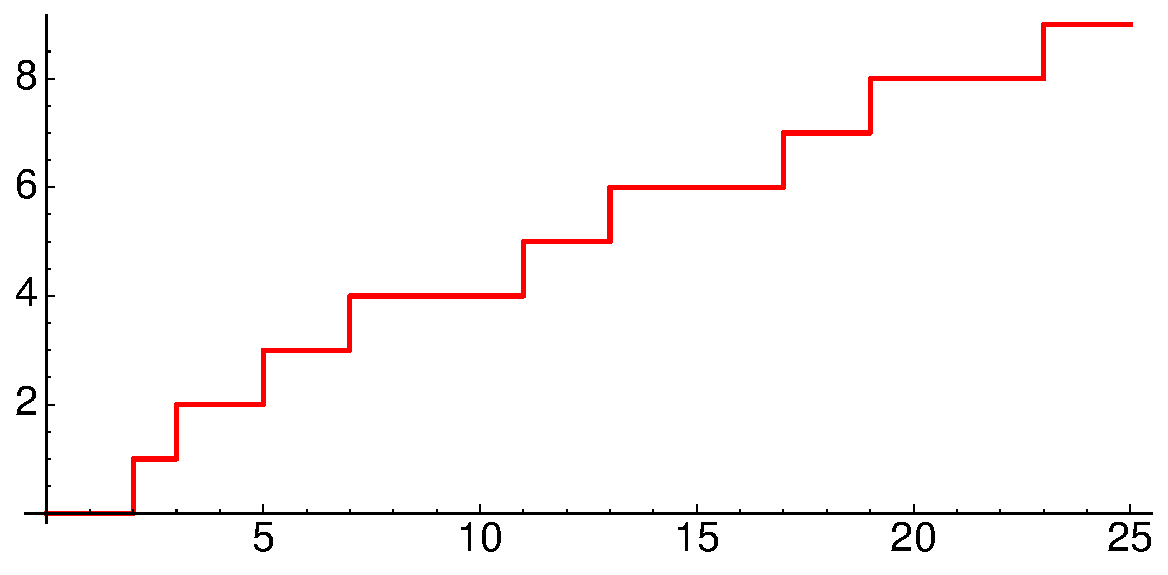
\includegraphics[width=.4\textwidth]{illustrations/PN_25}
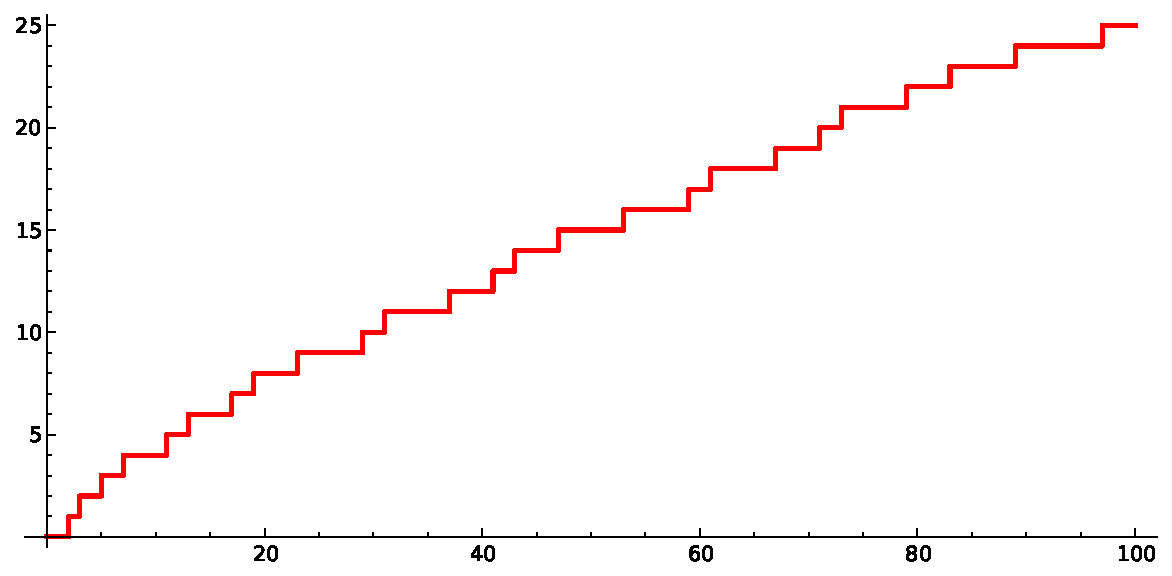
\includegraphics[width=.4\textwidth]{illustrations/PN_100}\\

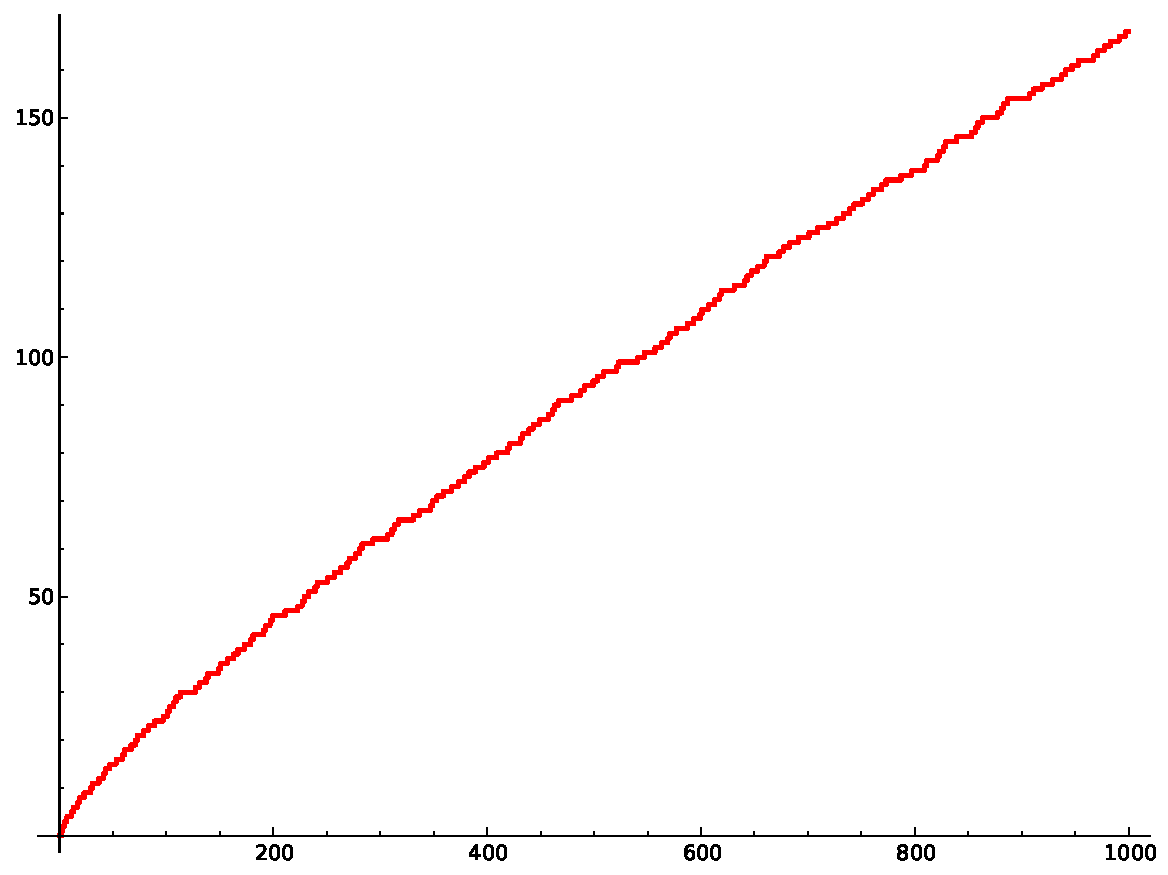
\includegraphics[width=.4\textwidth]{illustrations/PN_1000}
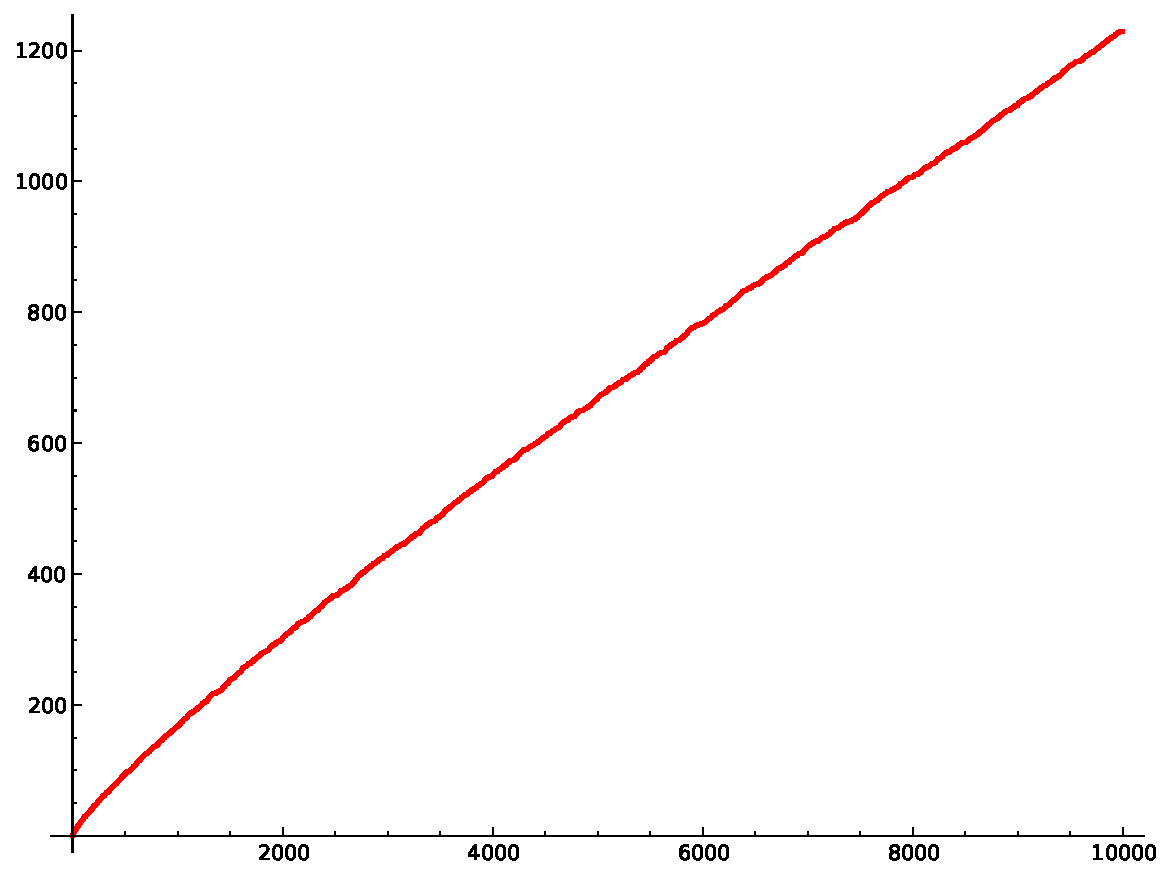
\includegraphics[width=.4\textwidth]{illustrations/PN_10000}\\

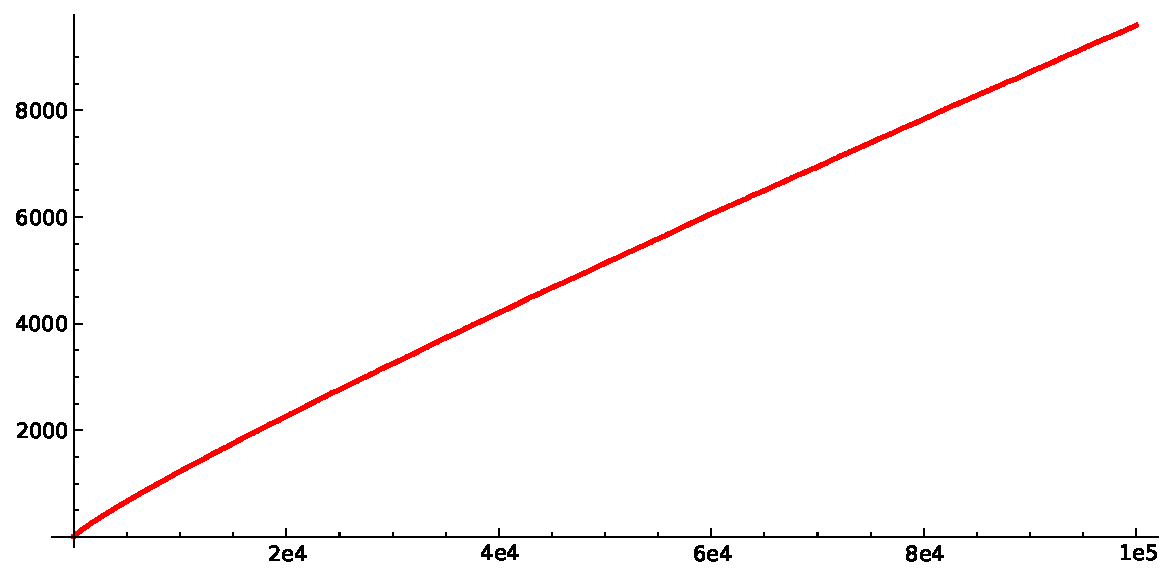
\includegraphics[width=.6\textwidth]{illustrations/PN_100000}


\caption{The Staircase of Primes\label{fig:staircases}}
\end{figure}

The mystery of this staircase is that the {\em information} contained
within it is---in effect---the full story of where the primes are
placed. This story seems to elude any simple description.  Can we
``tinker with'' this staircase without destroying this valuable
information?




\chapter[Tinkering with the staircase of primes]{Tinkering with the carpentry of the staircase of primes\label{sec:tinkering}}


For starters, notice that all the {\em risers} of this staircase (Figure~\ref{fig:staircases} above) have
unit length. That is, they contain no numerical information except for
their placement on the $x$-axis. So, we could distort our staircase by
changing (in any way we please) the height of each riser; and as long
as we haven't brought new risers into---or old risers out
of---existence, and have not modified their position over the
$x$-axis, we have retained all the information of our original
staircase.


A more drastic-sounding thing we could do is to judiciously add new
steps to our staircase. At present, we have a step at each prime
number $p$, and no step anywhere else. Suppose we built a staircase
with a new step not only at $x=p$ for $p$ each prime number but also at
$x =1$ and $x=p^n$ where $p^n$ runs through all powers of prime numbers as
well. Such a staircase would have, indeed, many more steps than our
original staircase had, but, nevertheless, would retain much of the
quality of the old staircase: namely it contains within it the full
story of the placement of primes {\em and their powers}.

A final thing we can do is to perform a distortion of the $x$-axis
(elongating or shortening it, as we wish) in any specific way, as long
as we can perform the inverse process, and ``undistort'' it if we wish.
Clearly such an operation may have mangled the staircase, but hasn't destroyed
information irretrievably.

We shall perform all three of these kinds of operations eventually,
and will see some great surprises as a result.  But for now, we will
perform distortions only of the first two types.  We are about to
build a new staircase that retains the precious information we need,
but is constructed according to the following architectural plan.

 \begin{itemize}

 \item We first build a staircase that has a new step precisely at $x
   =1$, and $ x= p^n$ for every {\em prime power} $p^n$ with $n\geq
   1$. That is, there will be a new step at $x= 1,2,3,4,5,7,8,9,11,
   \dots$

 \item Our staircase starts on the ground at $x=0$ and the height of the
   riser of the step at $x=1$ will be $\log(2\pi)$. The length of the
   riser of the step at $x=p^n$ will not be $1$
   (as was the length of all risers in the old staircase of primes)
   but rather: the step at $x=p^n$ will have the height of its riser
   equal to $\log p$.  So for the first few steps listed in the
   previous item, the risers will be of length $\log(2\pi), \log
   2,\log 3,\log 2,\log 5,\log 7, \log 2,\log 3,\log 11, \dots$
   Since $\log(p)>1$,
  these vertical dimensions lead to a steeper ascent but no great loss
  of {\em information}.

   Although we are not quite done with our architectural work, Figure~\ref{fig:psi} shows
   what our staircase looks like, so far.

\illtwo{psi_9}{psi_100}{.45}{The newly constructed staircase that counts prime powers\label{fig:psi}}


  \end{itemize}

  Notice that this new staircase looks, from afar, as if it were
  nicely approximated by the $45$ degree straight line, i.e., by the
  simple function $X$. In fact, we have---by this new
  architecture---a second {\em equivalent} way of formulating
  Riemann's hypothesis.   For this, let $\psi(X)$ denote the
  function
  of $X$ whose graph is
depicted in Figure~\ref{fig:psi}
(see \bibnote{We have $$\psi(X) =\sum_{p^n \le X}\log p$$ where the summation is over prime
powers $p^n$ that are $\le X$.}).

          \begin{center}
       \shadowbox{ \begin{minipage}{0.9\textwidth}
\mbox{}       \vspace{0.2ex}
       \begin{center}{\bf\large The {\bf \RH{}} (second formulation)}\end{center}
       \medskip

       This new staircase is essentially square root close to the 45 degree
straight line; i.e., the function $\psi(X)$ is essentially square root
close to the function $f(X)=X$.
          \vspace{1ex}
   \end{minipage}}
\end{center}

\ill{psi_diag_1000}{0.5}{The newly constructed staircase is close to the 45 degree line.}

Do not worry if you do not understand why our first and second
formulations of Riemann's Hypothesis are equivalent. Our aim, in
offering the second formulation---a way of phrasing Riemann's guess
that mathematicians know to be equivalent to the first one---is to
celebrate the variety of equivalent ways we have to express Riemann's
proposed answers to the question ``How many primes are there?'' and to
point out that some formulations would reveal a startling
simplicity---not immediately apparent---to the behavior of prime
numbers, no matter how erratic primes initially appear to us to
be. After all, what could be simpler than a 45 degree straight line?




\chapter[Computer music files and prime numbers]{What do  computer music files,
data compression, and prime numbers have to do with each other?\label{sec:fourier1}}




Sounds of all sorts---and in particular the sounds of music---travel
as vibrations of air molecules at roughly 768 miles an hour. These
vibrations---fluctuations of pressure---are often represented, or
``pictured,'' by a graph where the horizontal axis corresponds to
time, and the vertical axis corresponds to pressure at that time.  The
very purest of sounds---a single sustained note---would look
something like this (called a ``sine wave'') when pictured (see
Figure~\ref{fig:sine}), so that if you fixed your position somewhere
and measured air pressure due to this sound at that position, the
peaks correspond to the times when the varying air pressure is maximal
or minimal and the zeroes to the times when it is normal pressure.

\ill{sin}{.6}{Graph of a Sine Wave\label{fig:sine}}

You'll notice that there are two features to the graph in Figure~\ref{fig:sine}.

\begin{enumerate}
\item {\em The height of the peaks of this sine wave:} This height is
  referred to as the {\bf amplitude} and corresponds to the {\em
    loudness} of the sound.
\item {\em The number of peaks per second:} This number is referred to
  as the {\bf frequency} and corresponds to the {\em pitch} of the
  sound.
\end{enumerate}


Of course, music is rarely---perhaps never---just given by a single
pure sustained note and nothing else. A next most simple example of a
sound would be a simple chord (say a C and an E played together on
some electronic instrument that could approximate pure notes). Its
graph would be just the {\em sum} of the graphs of each of the pure
notes (see Figures~\ref{fig:sinetwofreq} and \ref{fig:sinetwofreqsum}).


\ill{sin-twofreq}{0.6}{Graph of Two Sine Waves with Different Frequencies\label{fig:sinetwofreq}}

\ill{sin-twofreq-sum}{.6}{Graph of Sum of the Two Sine Waves with Different Frequencies\label{fig:sinetwofreqsum}}

So the picture of the changing frequencies of this chord would be
already a pretty complicated configuration.  What we have described in
these graphs are two sine waves (our C and our E) when they are played
{\em in phase} (meaning they start at the same time) but we could
also ``delay'' the onset of the E note and play them with some
different phase relationship, for example, as illustrated
in Figures~\ref{fig:sin-twofreq-phase} and \ref{fig:sum-sin-phase}.

\ill{sin-twofreq-phase}{.6}{\label{fig:sin-twofreq-phase}Graph of two ``sine'' waves with different phase.}

\ill{sin-twofreq-phase-sum}{.6}{Graph of the sum of the two ``sine'' waves with different frequency
and phase.\label{fig:sum-sin-phase}}


  So, {\em all you need} to reconstruct the chord graphed above is to
  know five numbers:
  \begin{itemize}
  \item the two frequencies---the collection of frequencies that make
    up the sound is called the {\em spectrum} of the sound,
  \item the two {\em amplitudes} of each of these two frequencies,
  \item the {\em phase} between them.

 \end{itemize}

 Now suppose you came across such a sound as pictured in
 Figure~\ref{fig:sum-sin-phase} and wanted to ``record it.''  Well,
 one way would be to sample the amplitude of the sound at many
 different times, as for example in Figure~\ref{fig:sum-sin-phase-sample}.

\ill{sin-twofreq-phase-sum-points}{.6}{Graph of sampling of a sound wave\label{fig:sum-sin-phase-sample}}

Then, fill in the rest of the points to obtain Figure~\ref{fig:sum-sin-phase-sample-fill}.

\ill{sin-twofreq-phase-sum-fill}{0.6}{Graph obtained from Figure~\ref{fig:sum-sin-phase-sample} by
filling in the rest of the points\label{fig:sum-sin-phase-sample-fill}}

But this sampling would take an enormous amount of storage space, at
least compared to storing five numbers, as explained above!
Current audio compact discs do their sampling 44,100 times a second to
get a reasonable quality of sound.

Another way is to simply record the {\em five} numbers: the {\em
  spectrum, amplitudes,} and {\em phase}.  Surprisingly, this seems to
be roughly the way our ear processes such a sound when we hear it \bibnote{%
We recommend downloading Dave Benson's marvelous book
{\em Music: A Mathematical Offering} from
\url{http://www.maths.abdn.ac.uk/~bensondj/html/music.pdf}.
This is free, and gives a beautiful account of the superb
mechanism of hearing, and of the mathematics of music.}.

  Even in this simplest of examples (our pure chord: the pure note C
  played simultaneously with pure note E) the {\em efficiency of data
    compression} that is the immediate bonus of analyzing the picture
  of the chords as built {\em just} with the five numbers giving {\em
    spectrum, amplitudes,} and {\em phase} is staggering.

\ill{fourier}{0.3}{Jean Baptiste Joseph Fourier (1768--1830)}

This type of analysis, in general, is called {\em Fourier Analysis}
and is one of the glorious chapters of mathematics.  One way of
picturing {\em spectrum} and {\em amplitudes} of a sound is by a bar
graph which might be called the {\em spectral picture} of the sound,
the horizontal axis depicting frequency and the vertical one depicting
amplitude: the height of a bar at any frequency is proportional to the
amplitude of that frequency ``in'' the sound.

So our CE chord would have the spectral picture in
Figure~\ref{fig:ce-spectral}.


\illtwo{sound-ce-general_sum}{sound-ce-general_sum-blips}{.4}
       {Spectral Picture of a CE chord\label{fig:ce-spectral}}


This spectral picture ignores the phase but is nevertheless a very
good portrait of the sound.  The spectral picture of a graph gets us
to think of that graph as ``built up by the superposition of a bunch
of pure waves,'' and if the graph is complicated enough we may very well
need {\em infinitely} many pure waves to build it up!  Fourier analysis is a
mathematical theory that allows us to start with any graph---we are
thinking here of graphs that picture sounds, but any graph will
do---and actually compute its spectral picture (and even keep track of
phases).


The operation that starts with a graph and goes to its spectral
picture that records the frequencies, amplitudes, and phases of the
pure sine waves that, together, compose the graph is called the {\em
  Fourier transform} and nowadays there are very fast procedures for
getting accurate {\em Fourier transforms} (meaning accurate spectral
pictures including information about phases) by
computer \bibnote{Discuss some good readable article on the Fast
  Fourier Transform algorithm; there are probably many such
  articles.}.


%If you pass to the worksheet at this point, you'll be able to see the
%Fourier transforms of many different sounds, and experiment for
%yourself.
The theory behind this operation (Fourier transform giving
us a spectral analysis of a graph) is quite beautiful, but equally
impressive is how---given the power of modern computation---you can
immediately perform this operation for yourself to get a sense of how
different wave-sounds can be constructed from the superposition of
pure tones.

The {\em sawtooth} wave in Figure~\ref{fig:sawtooth} has a spectral picture, its Fourier transform, given in Figure~\ref{fig:sawtooth-spectrum}:

   \ill{sawtooth}{.7}{Graph of Sawtooth Wave\label{fig:sawtooth}}
   \ill{sawtooth-spectrum}{.6}{The Spectrum of the Sawtooth Wave Has a Spike of Height $1/k$ at
each integer $k$\label{fig:sawtooth-spectrum}}



 \ill{complicated-wave}{.6}{A Complicated Sound Wave\label{fig:complicated-wave}}

Suppose you have a complicated sound wave, say as in
Figure~\ref{fig:complicated-wave}, and you want to record it.
Standard audio CD's record their data by intensive sampling as we
mentioned. In contrast, current mp3 audio compression technology uses
Fourier transforms plus sophisticated algorithms based on
knowledge of which frequencies the human ear can hear.
With this, mp3 technology manages to
get a compression factor of 8--12 with little {\em perceived} loss in
quality, so that you can fit your entire music collection on your
mp3 player, instead of just a few of your favorite CD's.

\chapter{The word `Spectrum'}

% TODO: this is from wikipedia -- requires attribution.
\begin{wrapfigure}{r}{0.2\textwidth}
    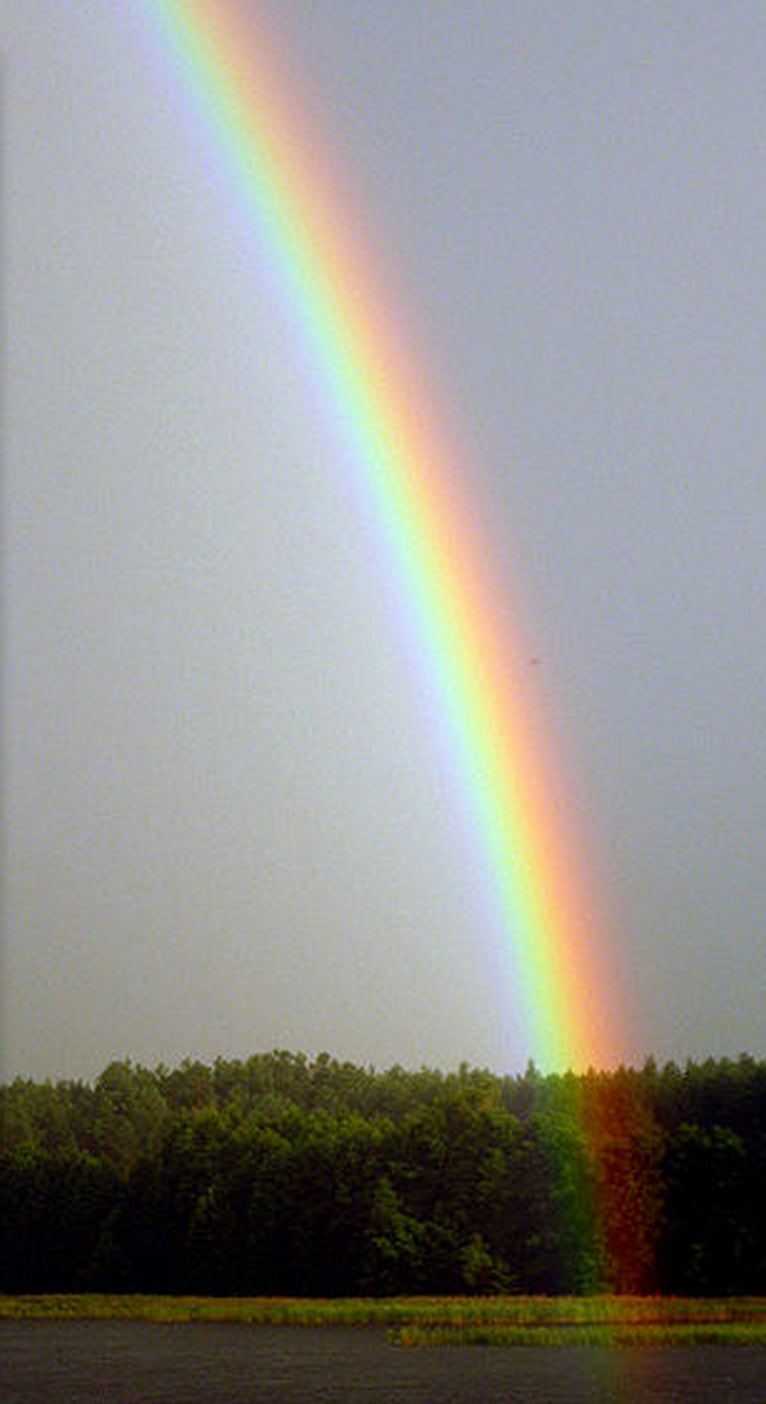
\includegraphics[width=0.2\textwidth]{illustrations/rainbow}
\end{wrapfigure}

  It is worth noting how often this word appears in scientific literature, with an array of different uses and meanings.   It  comes from Latin where its meaning is ``image," or ``appearance," related to the verb meaning {\it to look} (the older form being  {\it specere} and the later form {\it spectare}).  In most of its meanings, nowadays, it has to do with some procedure, an analysis, allowing one to see clearly the  constituent parts of something to be analyzed, these constituent parts often organized in some continuous scale, such as in the discussion of the previous chapter.

  The Oxford Dictionary lists, as one of its many uses:

\begin{quote} Used to classify something, or suggest that it can be classified, in terms of its position on a scale between two extreme or opposite points.\end{quote}

This works well for the color spectrum, as initiation by Newton (as in the figure above, sunlight is separated by a prism into a rainbow  continuum of colors): an analysis of white light into its components. Or in mass spectrometry, where
 beams of ions are separated (analyzed) according to their
mass/charge ratio and the mass spectrum is recorded on a photographic plate or film.  Or in the recording of the various component frequencies, with their  corresponding intensities of some audible phenomenon.

 In mathematics the word  has found its use in many different fields, the most basic use occurring in Fourier analysis, which has as its goal the aim of either {\it analyzing}  a function $f(t)$ as being  comprised of simpler (specifically: sine and cosine) functions, or {\it synthesizing} such a function by combining simpler functions to produce it. The understanding here and in the previous chapter, is that  an analysis of $f(t)$ as built up of simpler functions is meant to provide a significantly clearer image of the constitution of $f(t)$.  If, to take a very particular example, the simpler functions  that are needed for the synthesis of $f(t)$ are of the form $a\cos(\theta t)$  (for $a$ some real number which is the {\it amplitude} or size of the peaks of this periodic function)---and  if $f(t)$ is given as the limit of $$a_1\cos(\theta_1t) +  a_2\cos(\theta_2t) + a_3cos(\theta_3t) \dots$$  for a sequence of real numbers $\theta_1, \theta_2,
 \theta_3,
 \dots$  (i.e., these simpler functions are functions of {\it periods} ${\frac{2\pi}{\theta_1}}, {\frac{2\pi}{\theta_2}}, {\frac{2\pi}{\theta_3}}, \dots$) it is natural to call the these $\theta_i$ the  {\bf spectrum} of $f(t)$.
   This will eventually show up in our discussion  below of trigonometric sums and the {\it Riemann Spectrum}.


 \chapter{Spectra and Trigonometric Sums \label{sec:trigsums}}

As we saw in Chapter~\ref{sec:fourier1}, a pure tone can be represented by a periodic {\it sine wave}---a function of  time $f(t)$--- the equation of which might be:
$$f(t)\ \ = \ \ a\cdot \cos(b +\theta t).$$

\ill{pure_tone}{.7}{Plot of the periodic sine wave $f(t) = 2\cdot \cos(1+t/2)$}

The $\theta$ determines the {\it frequency} of the periodic wave, the
larger $\theta$ is the higher the ``pitch.''  The coefficient $a$
determines the envelope of size of the periodic wave, and we call it
the {\it amplitude} of the periodic wave.

Sometimes we encounter functions $F(t)$ that are not pure tones, but
that can be expressed as (or we might say ``decomposed into'') a finite
sum of pure tones, for example three of them:

$$F(t)  = a_1\cdot \cos(b_1 +\theta_1 t) + a_2\cdot \cos(b_2 +\theta_2 t) + a_3\cdot \cos(b_3 +\theta_3 t)$$

\ill{mixed_tone3}{.7}{Plot of the sum $5  \cos\left(-t - 2\right) + 2 \cos\left(t/2 + 1\right) + 3  \cos\left(2  t + 4\right)$}

We'll refer to such functions $F(t)$ as {\it finite trigonometric
  sums}, because ---well---they are.  In this example, there are three
frequencies involved---i.e., $\theta_1,\theta_2,\theta_3$---and we'll
say that {\it the spectrum of $F(t)$} is the set of these frequencies,
i.e.,

$$
  {\rm The\ spectrum \ of \ } F(t) \ \ = \ \ \{\theta_1,\theta_2,\theta_3\}.
$$

More generally we might consider a sum of any finite number of pure
cosine waves---or in a moment we'll also see some infinite ones as
well. Again, for these more general trigonometric sums, their {\it
  spectrum} will denote the set of frequencies that compose them.

\chapter{The spectrum and the staircase of primes\label{sec:fourier_staircase}}

\ill{prime_pi_100_aspect1}{0.95}{The Staircase of Primes\label{fig:staircase100}}


In view of the amazing data-compression virtues of Fourier analysis,
it isn't unnatural to ask these questions:

\begin{itemize}
\item Is there a way of using Fourier analysis to better understand
  the complicated picture of the staircase of primes?

\item Does this staircase of primes (or, perhaps, some tinkered
  version of the staircase that contains the same basic information)
  have a {\it spectrum}?

\item If such a {\it spectrum} exists, can we compute it conveniently,
  just as we have done for the saw-tooth wave above, or for the major
  third CE chord?


\item Assuming the spectrum exists, and is computable, will our
  understanding of this spectrum allow us to reproduce all the
  pertinent information about the placement of primes among all whole
  numbers, elegantly and faithfully?

\item And here is a most important question: will that spectrum show
  us order and organization lurking within the staircase that we would
  otherwise be blind to?

\end{itemize}


Strangely enough, it is towards questions like these that Riemann's
Hypothesis takes us. We began with the simple question about primes:
how to count them, and are led to ask for profound, and hidden,
regularities in structure.

\chapter{To our readers of Part~\ref{part1}}
The statement of the \RH{}---admittedly as elusive as
before---has, at least, been expressed elegantly and more simply,
given our new staircase that approximates (conjecturally with {\em
  essential square root accuracy}) a 45 degree straight line.

We have offered two equivalent formulations of the \RH{},
both having to do with the manner in which the prime numbers are
situated among all whole numbers.

In doing this, we hope that we have convinced you that---in the words
of Don Zagier---primes seem to obey no other law than that of chance
and yet exhibit stunning regularity.  This is the end of Part~\ref{part1} of our
book, and is largely the end of our main mission, to explain---in
elementary terms---{\em what is Riemann's Hypothesis?}


For readers who have at some point studied Differential Calculus, in
Part~\ref{part2} we shall discuss Fourier analysis, a fundamental tool that will be used in Part~\ref{part3}
where we show how
Riemann's hypothesis provides a key to some deeper structure of the
prime numbers, and to the nature of the laws that they obey. We will ---if not explain--at least
hint at how the above series of questions have been answered so far,
and how the \RH{} offers a surprise for the last question in this
series.



%\chapter{To our readers of Part~\ref{part1}}
%The statement of the \RH{}---admittedly as elusive as
%before---has, at least, been expressed elegantly and more simply,
%given our new staircase that approximates (conjecturally with {\em
 % essential square root accuracy}) a 45 degree straight line.

%We have offered two equivalent formulations of the \RH{},
%both having to do with the manner in which the prime numbers are
%situated among all whole numbers.

%In doing this, we hope that we have convinced you that---in the words
%of Don Zagier---primes seem to obey no other law than that of chance
%and yet exhibit stunning regularity.  This is the end of Part~\ref{part1} of our
%book, and is largely the end of our main mission, to explain---in
%elementary terms---{\em what is Riemann's Hypothesis?}


%For readers who have at some point studied Differential Calculus, in
%Part~\ref{part2} we shall
%go further and explain how the pursuit of
%Riemann's hypothesis may provide a key to some deeper structure of the
%prime numbers, and to the nature of the laws that they obey.


\part{Distributions\label{part2}}


\chapter[Slopes of graphs that have no slopes]{How Calculus manages to
  find the slopes of graphs that have no slopes}

Differential Calculus, initially the creation of Newton and/or Leibniz
in the 1680s, acquaints us with {\it slopes} of graphs of functions of
a real variable.  So, to discuss this we should say a word about what
a {\it function} is, and what its {\it graph} is.

 \illtwo{newton}{leibniz}{0.25}{Isaac Newton and Gottfried Leibniz created Calculus}


 A {\bf function} (let us refer to it in this discussion as $f$) is
 often described as a {\it kind of machine} that for any specific
 input numerical value $a$ will give, as output, a well-defined
 numerical value.

 This ``output number'' is denoted $f(a)$ and is called {\it the
   ``value'' of the function $f$ at $a$}.  For example, the {\it
   machine that adds $1$ to any number} can be thought of as the
 function $f$ whose value at any $a$ is given by the equation $f(a) =
 a+1$.  Often we choose a letter---say, $X$---to stand for a ``general
 number'' and we denote the function $f$ by the symbol $f(X)$ so that
 this symbolization allows to ``substitute for $X$ any specific number
 $a$'' to get its value $f(a)$.

 The {\bf graph} of a function provides a vivid visual representation of the
 function in the Euclidean plane where over every point $a$ on the
 $x$-axis you plot a point above it of ``height'' equal to the value of
 the function at $a$, i.e., $f(a)$. In Cartesian coordinates, then,
 you are plotting points $(a, f(a))$ in the plane where $a$ runs
 through all real numbers.

 \ill{graph_aplusone}{0.6}{Graph of the function $f(a)=a+1$\label{fig:graph_aplusone}}

 In this book we will very often be talking about ``graphs'' when we
 are also specifically interested in the functions---of which they are
 the graphs. We will use these words almost synonymously since we like
 to adopt a very visual attitude towards the behavior of the functions
 that interest us.


 \ill{graph_slope_deriv}{0.7}{\label{fig:graph_slope_deriv}Calculus}



 Figure~\ref{fig:graph_slope_deriv} illustrates a function (blue), the
 slope at a point (black straight line), and the derivative (red) of
 the function; the red derivative is the function whose value at a point
 is the slope of the blue function at that point.  Differential
 Calculus explains to us how to calculate slopes of graphs, and
 finally, shows us the power that we then have to answer problems we
 could not answer if we couldn't compute those slopes.

Usually, in elementary Calculus classes we are called upon to compute
slopes only of smooth graphs, i.e., graphs that actually {\em have}
slopes at each of their points, such as in the illustration just
above.  What could Calculus possibly do if confronted with a graph
that has {\em jumps}, such as in Figure~\ref{fig:jump}:
$$f(x) = \begin{cases}1 & x \leq 3\\ 2 & x > 3.\end{cases}$$
(Note that for purely aesthetic reasons, we draw a vertical line at the point where the jump occurs, though technically that vertical line is not part of the graph of the function.)

\ill{jump}{0.5}{The graph of the function $f(x)$ above that jumps---it is $1$ up to $3$ and then $2$ after that point.\label{fig:jump}}


The most comfortable way to deal with the graph of such a function is
to just approximate it by a differentiable function as in
Figure~\ref{fig:jumpsmooth}.  Note that the function in
Figure~\ref{fig:jumpsmooth} is not smooth, since the
derivative is continuous but not differentiable; in our
discussion all
we will need is that our approximating function is once
differentiable.


\ill{jump-smooth}{0.5}{A picture of a smooth graph approximating the
  graph that is $1$ up to some point $x$ and then $2$ after that
  point, the smooth graph being flat mostly.\label{fig:jumpsmooth}}


Then take the {\em derivative} of that smooth function.  Of course,
this is just an approximation, so we might try to make a better
approximation, which we do in each successive graph starting
with Figure~\ref{fig:djump1} below.


\ill{jump-smooth-deriv-7}{0.6}{A picture of the derivative of
a smooth approximation to a function that jumps.\label{fig:djump1}}

Note that---as you would expect---in the range where the initial
function is constant, its derivative is zero. In the subsequent
figures, our initial function will be {\it nonconstant} for smaller
and smaller intervals about the origin. Note also that, in our series
of pictures below, we will be successively rescaling the $y$-axis; all
our initial functions have the value $1$ for ``large'' negative numbers
and the value $2$ for large positive numbers.

\ill{jump-smooth-deriv-2}{0.5}{Second picture of the derivative of
a smooth approximation to a function that jumps.\label{fig:djump2}}
\ill{jump-smooth-deriv-05}{0.5}{Third picture of the derivative of
a smooth approximation to a function that jumps.\label{fig:djump3}}
\ill{jump-smooth-deriv-01}{0.5}{Fourth picture of the derivative of
a smooth approximation to a function that jumps.\label{fig:djump4}}


Notice what is happening: as the approximation gets better and
better, the derivative will be zero mostly, with a blip at the point
of discontinuity, and the blip will get higher and higher.
In each of these pictures,  for any interval of real numbers $[a,b]$ the total area under the red graph over that interval is equal to
\begin{center}
{\it the height of the blue graph at $x=b$}\\
minus\\
{\it  the height of the blue graph  at $x=a$}.
\end{center}
This is a manifestation of one of the fundamental facts of life of
Calculus relating a function to its derivative:

\begin{quote} Given any real-valued function $F(x)$---that has a
  derivative---for any interval of real numbers $[a,b]$ the total area
  under the graph of the derivative of $F(x)$ over that interval is
  equal to $F(b)-F(a)$.
  \end{quote}
    What happens if we take the series of figures \ref{fig:djump1}--\ref{fig:djump4}, etc.
    {\it to the limit}?  This is quite curious:

  \begin{itemize}
  \item {\bf the series of red graphs:} these are getting thinner and
    thinner and higher and higher: can we make any sense of what the
    red graph might mean in the limit (even though the only picture of
    it that we have at present makes it infinitely thin and infinitely
    high)?

  \item {\bf the series of blue graphs:} these are happily looking
    more and more like the tame Figure~\ref{fig:jump}.
   \end{itemize}

   Each of our red graphs is the derivative of the corresponding blue
   graph. It is tempting to think of the limit of the red
   graphs---whatever we might construe this to be---as standing for
   the derivative of the limit of the blue graphs, i.e., of the graph
   in Figure~\ref{fig:jump}.

   Well, the temptation is so great that, in fact, mathematicians and
   physicists of the early twentieth century struggled to give a
   meaning to things like {\it the limit of the red graphs}---such
   things were initially called {\bf generalized functions} which
   might be considered the derivative of {\it the limit of the blue
     graphs}, i.e., of the graph of Figure~\ref{fig:jump}.


   Of course, to achieve progress in mathematics, all the concepts
   that play a role in the theory have to be unambiguously defined,
   and it took a while before {\it generalized functions} such as the
   limit of our series of red graphs had been rigorously introduced.

   But many of the great moments in the development of mathematics
   occur when mathematicians---requiring some concept not yet
   formalized---work with the concept tentatively, dismissing---if
   need be---mental tortures, in hopes that the experience they
   acquire by working with the concept will eventually help to put
   that concept on sure footing. For example, early mathematicians
   (Newton, Leibniz)|in replacing approximate speeds by instantaneous
   velocities by passing to limits|had to wait a while before later
   mathematicians (e.g., Weierstrass) gave a rigorous foundation for
   what they were doing.


 % From http://en.wikipedia.org/wiki/Karl_Weierstrass

% From http://en.wikipedia.org/wiki/Laurent_Schwartz
 \illtwo{weierstrass}{schwartz}{.3}{Karl Weierstrass (1815--1897) and Laurent Schwartz (1915--2002)}

 Karl Weierstrass, who worked during the latter part of the nineteenth
 century, was known as the ``father of modern analysis.'' He oversaw
 one of the glorious moments of rigorization of concepts that were
 long in use, but never before systematically organized.  He, and
 other analysts of the time, were interested in providing a rigorous
 language to talk about {\it functions} and more specifically {\it
   continuous functions} and {\it smooth} (i.e., {\it differentiable})
 functions. They wished to have a firm understanding of limits (i.e.,
 of sequences of numbers, or of functions).


 For Weierstrass and his companions, even though the functions they
 worked with needn't be smooth, or continuous, at the very least, the
 functions they studied had {\it well-defined---and usually
   finite---values}.  But our ``limit of red graphs'' is not so easily
 formalized as the concepts that occupied the efforts of
 Weierstrass.

 Happily however, this general process of approximating
 discontinuous functions more and more exactly by smooth functions,
 and taking their derivatives to get the blip-functions as we have
 just seen in the red graphs above was eventually given a
 mathematically rigorous foundation; notably, by the French
 mathematician, Laurent Schwartz who provide a beautiful theory that
 we will not go into here, that made perfect sense of ``generalized
 functions'' such as our limit of the series of red graphs, and that
 allows mathematicians to work with these concepts with ease. These
 ``generalized functions'' are called {\it distributions} in
 Schwartz's theory \bibnote{ See
   \url{http://en.wikipedia.org/wiki/Distribution_\%28mathematics\%29}
   for more about distributions.  Also, Schwartz's explains on page 238
   of his autobiography: ``Why did we choose the name distribution?
   Because, if $\mu$ is a measure, i.e., a particular kind of
   distribution, it can be considered as a distribution of electric
   charges in the universe.  Distributions give more general types of
   electric charges, for example dipoles and magnetic distributions.
   If we consider the dipole placed at the point $a$ having magnetic
   moment $M$, we easily see that it is defined by the distribution
   $-D_M \delta_{(a)}$.  These objects occur in physics.  Deny's
   thesis, which he defended shortly after, introduced electric
   distributions of finite energy, the only ones which really occur in
   practice; these objects really are distributions, and do not
   correspond to measures.  Thus, distributions have two very
   different aspects: they are a generalization of the notion of
   function, and a generalization of the notion of distribution of
   electric charges in space. [...] Both these interpretations of
   distributions are currently used.''}.




\chapter[Distributions]{Distributions: sharpening our approximating functions even if
  we have to let them shoot out to infinity\label{sec:dist}}



The curious {\it limit of the red graphs} of the previous section,
which you might be tempted to think of as a ``blip-function'' that
vanishes for $t$ nonzero and is somehow ``infinite'' (whatever that
means) at $0$ is an example of a {\it generalized function} (in the
sense of the earlier mathematicians) or a {\it distribution} in the
sense of Laurent Schwartz.

This particular {\it limit of the red graphs} also goes by another
name (it is officially called a Dirac $\delta$-function, the adjective
``Dirac'' being in honor of the physicist who first worked with this
concept, the ``$\delta$'' being the symbol he assigned to these
objects). The noun ``function'' should be in quotation marks for,
properly speaking, the Dirac $\delta$-function is not---as we have
explained above---a bona fide function but rather a distribution.

      \ill{dirac}{0.3}{Paul Adrien Maurice Dirac (1902--1984)}


      Now may be a good time to summarize what the major difference is
      between {\it honest functions} and {\it generalized functions}
      or {\it distributions}.

      An honest (by which we mean {\it integrable}) function of a real
      variable $f(t)$ possesses two ``features.''


\begin{itemize}
\item {\bf It has values.}  That is, at any real number $t$, e.g., $t
  =2$ or $t =0$ or $t =\pi$ etc., our function has a definite real
  number value ($f(2)$ or $f(0)$ or $f(\pi)$ etc.) {\it and if we know
    all those values we know the function.}

\item {\bf It has areas under its graph.} If we are given any interval
  of real numbers, say the interval between $a$ and $b$, we can talk
  unambiguously about the area ``under'' the graph of the function
  $f(t)$ over the interval between $a$ and $b$.  That is, in the
  terminology of Integral Calculus, we can talk of {\it the integral of $f(t)$
    from $a$ to $b$}.  And in the notation of Calculus, this---thanks
  to Leibniz---is elegantly denoted
$$\int_a^bf(t)dt.$$

\end{itemize}

   \ill{oo_integral}{.8}{This figure illustrates
      $\int_{-\infty}^{\infty} f(x) dx$, which is the signed area
      between the graph of $f(x)$ and the $x$-axis, where area below
      the $x$-axis (yellow) counts negative, and area above (grey) is
      positive.}


In contrast, a {\it generalized function}  or  {\it distribution}

\begin{itemize}
\item {\bf may not have ``definite values''} at all real numbers if it
  is not an honest function, nevertheless:

\item {\bf It has well-defined areas under portions of its ``graph.''}
  If we are given any interval of real numbers, say the (open)
  interval between $a$ and $b$, we can still talk unambiguously about
  the {\it area ``under'' the graph of the generalized function $D(t)$
    over the interval between $a$ and~$b$} and we will denote
  this--extending what we do in ordinary calculus---by the symbol
$$\int_a^bD(t)dt.$$
\end{itemize}

This description is important to bear in mind and it gives us a handy
way of thinking about ``generalized functions'' (i.e., distributions)
as opposed to functions: when we consider an (integrable) function of
a real variable, $f(t)$, we may invoke its {\it value} at every real
number and for every interval $[a,b]$ we may consider the quantity
$\int_a^bf(t)dt$. BUT when we are given a generalized function $D(t)$
we {\it only} have at our disposal the latter quantities.  In fact, a
generalized function of a real variable $D(t)$ is (formally) nothing
more than a {\it rule} that assigns to any finite interval $[a,b]$ ($a
\le b$) a quantity that we might denote $\int_a^bD(t)dt$ and that {\it
  behaves as if it were the integral of a function} and in
particular---for three real numbers $a\le b\le c$ we have the
additivity relation
 $$  \int_a^cD(t)dt \ = \ \int_a^bD(t)dt \ + \ \int_b^cD(t)dt.$$

 SO, any honest function integrable over finite intervals clearly {\it
   is} a distribution (forget about its values!) but $\dots$ there are
 many more generalized functions, and including them in our sights
 gives us a very important tool.


 It is natural to talk, as well, of Cauchy sequences, and limits, of
 distributions. We'll say that such a sequence $D_1(t), D_2(t),
 D_3(t),\dots$ is a {\bf Cauchy sequence} if for every interval
 $[a,b]$ the quantities $$\int_a^bD_1(t)dt,\quad
 \int_a^bD_2(t)dt,\quad\int_a^bD_3(t)dt,\dots$$ form a Cauchy sequence
 of real numbers. Now, any Cauchy sequence of distributions {\it
   converges to a limiting distribution} $D(t)$ which is defined by
 the rule that for every interval $[a,b]$,

  $$ \int_a^bD(t)dt\ =\ \lim_{i \to \infty} \int_a^bD_i(t)dt.$$


  If, by the way, you have an infinite sequence---say---of honest,
  continuous, functions that converges uniformly to a limit (which
  will again be a continuous function) then that sequence certainly
  converges---in the above sense---to the same limit when these
  functions are viewed as generalized functions. BUT, there are many
  important occasions where your sequence of honest continuous
  functions doesn't have that convergence property and {\it yet} when
  they are viewed as generalized functions they do converge to some
  generalized function as a limit. We will see this soon when we get
  back to the ``sequence of the red graphs.'' This sequence {\bf does}
  converge (in the above sense) to the Dirac $\delta$-function when
  these red graphs are thought of as a sequence of generalized
  functions.




  The integral notation for distribution is very useful, and allows us
  the flexibility to define, for nice enough---and honest---functions
  $c(t)$ useful expressions such as $$\int_a^bc(t)D(t).$$

 \ill{dirac_delta}{0.5}{The Dirac $\delta$-``function'' (actually
   distribution), where we draw a vertical arrow to illustrate the
   delta function with support at a given point.}

 For example, for the Dirac $\delta$-function we have been discussing
 (i.e., the limit of the red graphs of the previous section) {\it is}
 an honest function away from $t=0$ and ---in fact---is the ``trivial
 function'' zero away from the origin.  And at $0$, we may {\it say}
 that it has the ``value'' infinity, in honor of it being the limit of
 blip functions getting taller and taller at $0$ but the feature that
 pins it down as a distribution is given by its behavior relative to
 the second feature above, the area of its graph over the open
 interval between $a$ and $b$:

\begin{itemize}
\item If both $a$ and $b$ have the same sign (i.e., if the origin is
  not in the open interval spanned by $a$ and $b$) then the ``area
  under the graph of our Dirac $\delta$-function'' is $0$.
\item If $a$ is negative and $b$ is positive then the ``area under the
  graph of our Dirac $\delta$-function'' is $1$---in
  notation $$\int_a^b\delta = 1.$$
\end{itemize}




We sometimes summarize the fact that these areas vanish so long as the
origin is not included in the interval we are considering by saying
that the {\bf support} of this $\delta$-function is ``at the origin.''


Once you're happy with {\it this} Dirac $\delta$-function, you'll also
be happy with a Dirac $\delta$-function---call it $\delta_x$---with
support concentrated at any specific real number $x$ gotten by
``translating'' the one we've been talking about appropriately;
$\delta_x$ vanishes for $t \ne x$ and intuitively speaking, has an
{\it infinite blip} at $t=x$.

So, the original delta-function we were discussing, i.e., $\delta(t)$
would be denoted $\delta_0(t)$.

 \noindent {\bf A question:} If you've never seen distributions
 before, but know the Riemann integral, can you guess at what the
 definition of $\int_a^bc(t)D(t)$ is, and can you formulate hypotheses
 on $c(t)$ that would allow you to endow this expression with a
 definite meaning?


\noindent {\bf A second question:} if you have not seen distributions
before, and have answered the first question above, let
$c(t)$ be an honest function for which your definition
of $$\int_a^bc(t)D(t)$$ applies. Now let $x$ be a real number.
 Can you use your definition to compute

 $$\int_{-{\infty}}^{+{\infty}}c(t)\delta_x(t)?$$

 The answer, by the way, is:
 $\int_{-{\infty}}^{+{\infty}}c(t)\delta_x(t)=c(x).$ This will be useful in the later sections!


The theory of distributions gives a partial answer to the following funny question:


\begin{quote} How in the world can you ``take the derivative'' of a
  function $F(t)$ that doesn't have a derivative?
\end{quote}

The short answer to this question is that {\it this derivative $F'(t)$
  which doesn't exist as a function may exist as a distribution.}
What then is the integral of that distribution? Well, it is given by
the original function!

$$\int_a^bF'(t)dt \ = \ F(b) -F(a).$$

Let us practice this with simple staircase functions. For example,
what is the {\it derivative}---in the sense of the theory of
distributions---of the function in Figure~\ref{fig:simple_staircase}.
{\bf Answer} $\delta_0 + 2 \delta_1$.


\ill{simple_staircase}{.5}{The staircase function that is $0$ for $t
  \le 0$, $1$ for $0 <t \le 1$ and $3$ for $1< t \le 2$ has derivative
  $\delta_0 + 2\delta_1$.\label{fig:simple_staircase}}


We'll be dealing with much more complicated staircase functions in the
next section, but the general principles discussed here will nicely
apply there \bibnote{ From Wikipedia:
  \begin{quote} ``Generalized functions'' were introduced by Sergei
    Sobolev in 1935. They were independently introduced in the late
    1940s by Laurent Schwartz, who developed a comprehensive theory of
    distributions.
\end{quote}
}.


\chapter{Fourier transforms: second visit}

In Chapter~\ref{sec:fourier1} above we wrote:

\begin{quote} The operation that starts with a graph and goes to its
  spectral picture that records the frequencies, amplitudes, and
  phases of the pure sine waves that, together, compose the graph is
  called the {\bf Fourier transform}.
\end{quote}


  Now let's take a closer look at this operation {\it Fourier transform}.

  We will focus our discussion on an {\bf even} function $f(t)$ of a
  real variable $t$.  ``{\bf Even}'' means that its graph is symmetric
  about the $y$-axis; that is, $f(-t)= f(t)$.  See
  Figure~\ref{fig:even_function}.

  \ill{even_function}{.8}{The graph of an even function is symmetrical
    about the $y$-axis.\label{fig:even_function}}

  When we get to apply this discussion to the {\it staircase of
    primes} $\pi(t)$ or the {\it tinkered staircase of primes}
  $\psi(t)$ both of which being defined only for positive values of
  $t$, then we would ``lose little information'' in our quest to
  understand them if we simply ``symmetrized their graphs'' by
  defining their values on negative numbers $-t$ via the formulas
  $\pi(-t)=\pi(t)$ and $\psi(-t)=\psi(t)$ thereby turning each of them
  into {\it even functions}.

\ill{even_pi}{.8}{Even extension of the staircase of primes.}

The idea behind the Fourier transform is to express $f(t)$ as {\it
  made up out of sine and cosine wave functions}.  Since we have
agreed to consider only even functions, we can dispense with the sine
waves---they won't appear in our Fourier analysis---and ask how to
reconstruct $f(t)$ as a {\it sum} (with coefficients) of cosine
functions (if only finitely many frequencies occur in the spectrum of
our function) or more generally, as an {\it integral} if the spectrum
is more elaborate.  For this work, we need a little machine that tells
us, for each real number $\theta$ whether or not $\theta$ is in the
spectrum of $f(t)$, and if so, what the amplitude is of the cosine
function $\cos(\theta t)$ that occurs in the Fourier expansion of
$f(t)$---this amplitude answers the awkwardly phrased question: {\it
  how much $\cos(\theta t)$ ``occurs in'' $f(t)$?}  We will denote this
amplitude by ${\hat f}(\theta)$, and refer to it as {\bf the Fourier
  transform} of $f(t)$.  The {\bf spectrum}, then, of $f(t)$ is the
set of all frequencies $\theta$ where the amplitude is nonzero.


\ill{fourier_machine}{.6}{The Fourier Transform Machine, which transforms $f(t)$ into ${\hat f}(\theta)$\label{fig:fourier_machine}}


Now in certain easy circumstances---specifically, if
$\int_{-{\infty}}^{+{\infty}}|f(t)|dt$ (exists, and) is finite---the
Integral Calculus provides us with an easy construction of that
machine (see Figure~\ref{fig:fourier_machine}); namely:

    $${\hat f}(\theta) = \int_{-{\infty}}^{+{\infty}}f(t)\cos(-\theta t)dt.$$


    This concise machine manages to ``pick out'' just the part of
    $f(t)$ that has frequency $\theta$!!  It provides for us the {\it
      analysis} part of the Fourier analysis of our function
    $f(t)$.

    But there is a {\it synthesis} part to our work as well,
    for we can reconstruct $f(t)$ from its Fourier transform, by a
    process intriguingly similar to the analysis part; namely:  if
$\int_{-{\infty}}^{+{\infty}}|{\hat f}(\theta)|d\theta$ (exists, and) is finite, we retrieve $f(t)$ by the integral

      $$f(t)  = {\frac{1}{2\pi}}\int_{-{\infty}}^{+{\infty}}{\hat f}(\theta)\cos(\theta t)d\theta.$$

      We are not so lucky to have
      $\int_{-{\infty}}^{+{\infty}}|f(t)|dt$ finite when we try our
      hand at a Fourier analysis of the staircase of primes, but we'll
      work around this!



\chapter[Fourier transform of delta]{What is the Fourier transform of a delta function?\label{sec:ftdelta}}

Consider the $\delta$-function that we denoted $\delta(t)$ (or
$\delta_0(t)$). This is also the ``generalized function'' that we
thought of as the ``limit of the red graphs'' in Chapter~\ref{sec:dist}
above. Even though $\delta(t)$ is a distribution and {\it not} a bona
fide function, it is symmetric about the origin, and
also $$\int_{-{\infty}}^{+{\infty}}|\delta(t)|dt$$ exists, and is
finite (its value is, in fact, $1$). All this means that,
appropriately understood, the discussion of the previous section
applies, and we can {\it feed} this delta-function into our Fourier
Transform Machine (Figure~\ref{fig:fourier_machine}) to see what
frequencies and amplitudes arise in our attempt to express---whatever
this means!---the delta-function as a sum, or an integral, of cosine
functions.


     So what is the Fourier transform,  ${\hat \delta_0}(\theta)$, of the delta-function?


Well, the general formula would give us:
  $$ {\hat \delta_0}(\theta) = \int_{-\infty}^{+\infty}\cos(-\theta t)\delta_0(t)dt$$
  and as we mentioned in section 18, for any nice function $c(t)$ we
  have that the integral of the product of $c(t)$ by the distribution
  $\delta_x(t)$ is given by the {\it value} of the function $c(t)$ at
  $t=x$.  SO:

$$ {\hat \delta_0}(\theta) = \int_{-\infty}^{+\infty}\cos(-\theta t)\delta_0(t)dt = \cos(0) = 1.$$


In other words, the Fourier transform of $\delta_0(t)$ is the constant
function $$ {\hat \delta_0}(\theta)=1.$$ One can think of this
colloquially as saying that the delta-function is a perfect example of
{\it white noise} in that {\it every} frequency occurs in its Fourier
analysis and they all occur in equal amounts.

To generalize this computation let us consider for any real number $x$
the symmetrized delta-function with support at $x$ and $-x$, given
by $$d_x(t) \ = \ (\delta_x(t) + \delta_{-x}(t))/2$$


    \ill{two_delta}{0.4}{The sum $(\delta_x(t) + \delta_{-x}(t))/2$, where we draw vertical arrows to illustrate the Dirac delta functions.}

    What is the Fourier transform of this $d_x(t)$?  The answer is
    given by making the same computation as we've just made:

\begin{align*}\label{dx}
{\hat d_x}(\theta)  &=  {\frac{1}{2}}\left(\int_{-\infty}^{+\infty}\cos(-\theta t)\delta_x(t)dt + \int_{-\infty}^{+\infty}\cos(-\theta t)\delta_{-x}(t)dt\right)\\
    &= {\frac{1}{2}}\big(\cos(-\theta x)+ \cos(+\theta x)\big)\\
    &= \cos(x\theta)
\end{align*}


To summarize this in ridiculous (!) colloquial terms: {\it for any
  frequency $\theta$ the amount of $\cos(\theta t)$ you need to build
  up the generalized function $(\delta_x(t) + \delta_{-x}(t))/2$ is
  $\cos(x\theta).$ }


So far, so good, but remember that the theory of the Fourier transform
has---like much of mathematics---two parts: an {\it analysis part} and
a {\it synthesis} part.  We've just performed the {\it analysis} part
of the theory for these symmetrized delta functions $(\delta_x(t) +
\delta_{-x}(t))/2$.

Can we synthesize them---i.e., build them up again---from their Fourier transforms?


  We'll leave this, at least for now, as a question for you.

%\chapter{Supports, Spectra, Blips and Spikes}

%(to be written)

% Here is where we will
% be really justifying our heavy discussion of distributions,
% trigonometric sums, etc.

\chapter{Trigonometric series}\label{ch:trigseries}
Given our interest in the ideas of Fourier, it is not surprising that
we'll want to deal with things like $$F(\theta) = \sum_{k=1}^{\infty}
a_k\cos(s_k\cdot \theta)$$ where the $s_k$ are real numbers tending
(strictly monotonically) to infinity.  These we'll just call {\bf
  trigonometric series} without asking whether they converge in any
sense for all values of $\theta$, or even for {\it any} value of $\theta$. The
$s_k$'s that occur in such a trigonometric series we will call the
{\bf spectral values} or for short, the {\bf spectrum} of the series,
and the $a_k$'s the (corresponding) {\bf amplitudes}.  We repeat that
we impose no convergence requirements at all. But we also think of
these things as providing ``cutoff'' finite trigonometric sums, which
we think of as functions of two variables, $\theta$ and $C$ (the
``cutoff'') where $$F(\theta,C): = \sum_{s_k\le C} a_k\cos(s_k\cdot \theta).$$ These functions $F(\theta,C)$ are finite trigonometric series and therefore ``honest functions" having finite values everywhere.


\section{\bf Spike values} \begin{definition} Say
  that a trigonometric series $F(\theta)$ has a {\bf spike} at the real number $\theta=\tau \in {\bf R}$
if the set of absolute values $|F(\tau,C)|$  as $C$ ranges through positive number cutoffs is
  unbounded.  A real number $\tau \in {\bf R}$ is, in contrast, a {\bf
    non-spike} if those values admit a finite upper
  bound. \end{definition}

   One mission in this book will be furthered just by paying attention to the  spike values of certain (infinite) trigonometric series.
    The trigonometric sums we study are
  going to be particularly nice. Under the assumption of the Riemann
  Hypothesis, they  will have the
  property that the set of their spike values are particularly interesting {\it discrete}
  subsets of the real line.

\section{Trigonometric Series as Fourier Transforms}


Recall, as in Chapter \ref{sec:ftdelta}, that for any real number $x$, we considered
the symmetrized delta-function with support at $x$ and $-x$, given
by
$$
 d_x(t) \ = \ (\delta_x(t) + \delta_{-x}(t))/2,
$$
and noted that the Fourier transform of this $d_x(t)$  is
$$
   \label{dx2}{\hat d_x}(\theta)  = \cos(x\theta).
$$
\ill{two_delta}{0.4}{The sum $(\delta_x(t) + \delta_{-x}(t))/2$,
where we draw vertical arrows to illustrate the Dirac delta functions.}

It follows, of course, that a cutoff finite trigonometric series,
$F(\theta,C)$ associated to an infinite trigonometric series
$$
 F(\theta) = \sum_{k=1}^{\infty} a_k\cos(s_k\cdot \theta)
$$
is the Fourier transform of the distribution
$$
 D(t,C):=\sum_{s_k \le C}a_kd_{s_k}(t).
$$
Given the discreteness of the set of spectral values $s_k$ ($k=1,2,\dots$)  and
given the efficacy of  the theory of distributions, we can perfectly well
consider the infinite sum
$$
 D(t):=\sum_{k=1}^{\infty}a_kd_{s_k}(t),
$$ viewed as distribution, and playing the role of
the `inverse Fourier transform' of our trigonometric
series $F(t)$.


\part{The Riemann Spectrum of the Prime Numbers\label{part3}}

\chapter{ A sneak preview}\label{snpr}

To get a sense of what we're in for, let us consider two infinite trigonometric sums---that seem to be related one to the other in that the {\it frequencies} of the terms in the one trigonometric sum give the {\it spike values} of the other, and vice versa:   the {\it frequencies} of the other give the {\it spike values} of the one: a kind of duality as in the theory of Fourier transforms. We show this duality by exhibiting the graphs of more and more accurate finite approximations (cutoffs) of these infinite sums. More specifically,

\begin{enumerate}\item The first infinite trigonometric sum is a sum of pure cosine waves with frequencies given by {\it logarithms of powers of primes} and with amplitudes that will be described below. The graphs of longer and longer finite truncations of these trigonometric sums, as you will see, have ``higher and higher peaks" concentrated more and more accurately at a  {\it certain infinite discrete set of real numbers} that what we will be referring to as {\bf the Riemann spectrum} indicated in our pictures below (Figures~\ref{fig:pnsum5}-\ref{fig:pnsum500}) by the series of vertical red lines.

\item  In contrast, the second infinite trigonometric sum is a sum of pure cosine waves with frequencies given by what we have dubbed above {\it the Riemann spectrum} and with amplitudes all equal to $1$. These graphs will have ``higher and higher peaks" concentrated more and more accurately at {\bf the logarithms of powers of primes} indicated in our pictures below (see Figure~\ref{fig:phihat}) by the series of vertical blue lines.

               \end{enumerate}




That the series of {\it blue lines} (i.e., the logarithms of powers of
primes) in our pictures below determines---via the the trigonometric
sums we describe---the series of {\it red lines} (i.e., what we are
calling the spectrum) and conversely is a consequence of the Riemann
Hypothesis.
\begin{enumerate}

\item {\bf Getting the Riemann Spectrum as the spike values of a trigonometric series with
frequencies equal to (logs of) powers of the primes:}

  To get warmed up, let's plot the positive values of the following
  sum of (co-)sine waves:

    \begin{align*}
   f(t) =& -{\frac{\log(2)}{2^{1/2}}}\cos(t\log(2))- {\frac{\log(3)}{3^{1/2}}}\cos(t\log(3))\\
     &\qquad -{\frac{\log(2)}{4^{1/2}}}\cos(t\log(4))-{\frac{\log(5)}{5^{1/2}}}\cos(t\log(5))
  \end{align*}



\ill{mini_phihat_even}{1}{Plot of $f(t)$}


Look at the peaks of this graph. There is nothing very impressive
about them, you might think; but wait, for this is just a very ``early
'' piece of an expression that consists of a sum{\footnote{Here we
    make use of the Greek symbol $\sum$ as a shorthand way of
    expressing a sum of many terms.  We are not requesting this sum to
    converge.}}  of infinitely many (co-)sine waves:
$$
-\sum_{p^n}{\frac{\log(p)}{p^{n/2}}}\cos(t\log(p^n))
$$
the summation being over all powers $p^n$ of all prime numbers $p$.

Let us cut this infinite sum off taking only finitely many terms, by
choosing various ``cutoff values'' $C$ and forming the finite sums
$$
-\sum_{p^n\leq C}{\frac{\log(p)}{p^{n/2}}}\cos(t\log(p^n))
$$
and plotting their positive
values. Figures~\ref{fig:pnsum5}-\ref{fig:pnsum500} show what we get
for a few values of $C$.


In each of the graphs, we have indicated by red vertical arrows the
real numbers that give the values of the {\it Riemann spectrum} that we will
be discussing. These numbers at the red
vertical arrows in Figures~\ref{fig:pnsum5}--\ref{fig:phihat},
$$
\theta_1, \theta_2, \theta_3, \dots
$$
are  {\it spike values}---as described in Chapter~\ref{ch:trigseries}---of the infinite trigonometric series
$$
  -\sum_{p^n<C}{\frac{\log(p)}{p^{n/2}}} \cos(t \log(p^n)).
$$
They constitute what we are calling the Riemann spectrum and are key to the staircase of primes
\bibnote{If the \RH{} holds
they are precisely the  {\it imaginary parts of the
  ``nontrivial'' zeroes of the Riemann zeta-function}.}.

\begin{itemize}
\item {\bf The sum with $p^n \le C=5$}

Here is the function $f(t)$ we displayed above; it consists in the sum of the first four terms of our infinite sum, and doesn't yet show very much ``structure'':

\ill{phihat_even-5}{1}{Plot of $-\sum_{p^n\leq 5}{\frac{\log(p)}{p^{n/2}}}\cos(t\log(p^n))$ with
arrows pointing to the spectrum of the primes\label{fig:pnsum5}}

\vskip20pt
\item {\bf The sum with $p^n \le C=20$}

 Something,
 (don't you agree?)  is already beginning to happen here:
\ill{phihat_even-20}{1}{Plot of $-\sum_{p^n\leq 20}{\frac{\log(p)}{p^{n/2}}}\cos(t\log(p^n))$ with arrows pointing to the spectrum of the primes}\vskip20pt
\item {\bf The sum with $p^n \le C=50$}

  Note that the high peaks seem to be lining up more accurately with
  the vertical red lines. Note also that the $y$-axis has been
  rescaled.

\ill{phihat_even-50}{1}{Plot of $-\sum_{p^n\leq 50}{\frac{\log(p)}{p^{n/2}}}\cos(t\log(p^n))$ with arrows pointing to the spectrum of the primes}\vskip20pt
\item {\bf The sum with $p^n \le C=500$}

  Here, the peaks are even sharper, and note that again they are
  higher; that is, we have rescaled the $y$-axis.
  \ill{phihat_even-500}{1}{Plot of $-\sum_{p^n\leq
      500}{\frac{\log(p)}{p^{n/2}}}\cos(t\log(p^n))$ with arrows
    pointing to the spectrum of the primes\label{fig:pnsum500}}
\end{itemize}

  We will pay attention to:

\begin{itemize}
\item how this ``plays out'' as we take the sums of longer and longer
  pieces of the infinite sum of cosine waves above, given by larger
  and larger cutoffs $C$,
\item how this spectrum of red lines more closely matches the high
  peaks of the graphs of the positive values of these finite sums,
\item how these peaks are climbing higher and higher,
\item what relationship this has to the Fourier analysis of the
  staircase of primes,
\item and, equally importantly, what these mysterious red lines
  signify.
\end{itemize}

\item{\bf Towards (logs of) powers of the primes, starting from the Riemann Spectrum:}

  Here we will be making use of the series of numbers $$\theta_1,
  \theta_2, \theta_3, \dots$$ comprising what we called the {\it
    spectrum}. We consider the infinite trigonometric series
  $$
  1 + \cos(\theta_1t)+\cos(\theta_2t)+\cos(\theta_3t)+\dots
  $$
  or, using the $\sum$ notation,
 $$
  1+\sum_{\theta}\cos(\theta t)
 $$
 where the summation is over the spectrum, $\theta=\theta_1, \theta_2,
 \theta_3, \dots$. Again we will consider finite cutoffs $C$ of this
 infinite trigonometric sum, $${\hat \Phi}_{\le C}(\theta) = 1+\sum_{\theta\ \leq C}\cos(\theta t)$$
 and plot their graphs, over various ranges.

 \ill{phihat_even_all}{1}{Plots of ${\hat \Phi}_{\le C}(\theta)$ for
 $C=5$ (top), 20, 50, and 500 (bottom).\label{fig:phihat}}
\end{enumerate}

This passage---thanks to the Riemann Hypothesis--- from spectrum to
prime powers and back again via consideration of the ``high peaks'' in
the graphs of the appropriate trigonometric sums provides a kind of
visual duality emphasizing, for us, that the information inherent in
the wild spacing of prime powers, is somehow ``packaged'' in the series
of mysterious numbers we have called the Riemann Spectrum, and reciprocally,
the information given in that series of mysterious numbers is
obtainable from the sequence of prime powers.




\chapter{On losing no information\label{sec:loseno}}

To manage to repackage the ``same'' data in various ways---where each
way brings out some features that would be kept in the shadows if the
data were packaged in some different way---is a high art, in
mathematics. In a sense {\it every} mathematical equation does this,
for the ``equal sign'' in the middle of the equation tells us that
even though the two sides of the equation may seem different, or have
different shapes, they are nonetheless ``the same data.''  For
example, the equation

  $$\log(XY) = \log(X) + \log(Y)$$

  which we encountered earlier in Chapter~\ref{sec:firstguess}, is
  just two ways of looking at the same thing, yet it was the basis for
  much manual calculation for several centuries.




  Now, the problem we have been concentrating on, in this book, has
  been---in effect---to understand the pattern, if we can call it
  that, given by the placement of prime numbers among the natural
  line-up of all whole numbers.
\ill{primes_line}{1}{Prime Numbers up to $37$}

 There are, of course, many ways for us to present this basic
 pattern. Our initial strategy was to focus attention on the {\it
   staircase of primes} which gives us a vivid portrait, if you wish,
 of the order of appearance of primes among all numbers.
\ill{PN_38}{.45}{Prime Numbers up to $37$}

 As we have already hinted in the previous sections, however, there
 are various ways open to us to tinker with---and significantly
 modify---our staircase {\it without losing the essential information
   it contains}. Of course, there is always the danger of modifying
 things in such a way that ``retrieval'' of the original data becomes
 difficult.  Moreover, we had better remember every change we have
 made if we are to have any hope of retrieving the original data!

 With this in mind, let us go back to Chapter~\ref{sec:information}
 (discussing the staircase of primes) and Chapter~\ref{sec:tinkering},
 where we tinkered with the original staircase of primes---alias: the
 graph of $\pi(X)$---to get $\psi(X)$ whose risers look---from
 afar---as if they approximated the 45 degree staircase.% (see Figure~\ref{fig:psi38} below).


   At this point we'll do some further carpentry on $\psi(X)$ {\it without destroying the valuable
   information it contains}. We will be replacing  $\psi(X)$ by a generalized function, i.e., a
   distribution, which we denote $\Phi(t)$ that has support at all positive integral multiples
     of logs of prime numbers, and is  zero on the complement of that discrete set.  Recall that
     by definition, a discrete subset $S$ of real numbers is  the  {\bf support} of a function,
     or of a distribution, if the function vanishes on the complement of  $S$ and doesn't vanish
     on the complement of any proper subset of $S$.

   Given the mission of our book, it may be less important for us to  elaborate on  the construction
   of  $\Phi(t)$  than it is to {\bf (a)} note that $\Phi(t)$  contains all the valuable information
   that  $\psi(X)$ has and {\bf (b)} pay close attention to the spike values of the trigonometric
   series that is the Fourier transform of $\Phi(t)$.

     For the definition  of the distribution $\Phi(t)$ see the end-note
     \bibnote{
 {\it The construction of  $ \Phi(t)$ from $\phi(X)$:}

 Succinctly, for positive real numbers $t$, $$\Phi(t): \ = \ e^{- t/2}\Psi'(t),$$ where  $\Psi(t) = \phi(e^t)$,  and $\Psi'$ is the derivative of $\Psi(t)$ viewed as distribution. We extend this function to all real arguments $t$ by requiring $\Phi(t)$ to be an even function of $t$, i.e., $\Phi(-t)= \Phi(t)$. But, to review this in a more leisurely pace,
   \begin{enumerate}

   \item Distort the $X$-axis of our staircase by replacing the
     variable $X$ by $e^t$ to get the function $$\Psi(t):=
     \psi(e^t).$$ No harm is done by this for we can retrieve our
     original $\psi(X)$ as $$\psi(X) = \Psi(\log(X)).$$ Our distorted
     staircase has risers at ($0$ and) all positive integral multiples
     of logs of prime numbers.


%  \illtwo{psi_38}{bigPsi_38}{.4}{The two staircases $\psi$ (left) and $\Psi$ (right).  Notice that the plot of $\Psi$ on the  right is just the plot of $\psi$ but with the $X$-axis plotted on a logarithmic scale.\label{fig:psi38}}


\item Now we'll do something that might seem a bit more brutal: {\it
    take the derivative of this distorted staircase $\Psi(t)$.}  This
  derivative $\Psi'(t)$ is a {\it generalized} function with support
  at all nonnegative integral multiples of logs of prime numbers.

 \vskip20pt
 \ill{bigPsi_prime}{1}{$\Psi'(t)$ is a sum of Dirac delta functions at the logarithms of prime powers $p^n$ weighted by $\log(p)$ (and  $\log(2\pi)$ at $0$).  The more red the arrow, the larger the  weight.}

\item Now---for normalization purposes---multiply $\Psi'(t)$ by the
  function $e^{-t/2}$ which has no effect whatsoever on the support.
  \end{enumerate}
  \vskip20pt\ill{psi_200}{.6}{Illustration of the  staircase $\psi(x)$  constructed in Chapter~\ref{sec:tinkering} that counts weighted prime powers.\label{fig:psi_200}}

So what happens when we take the derivative---in the sense of
distributions---of a complicated staircase?  For example, see
Figure~\ref{fig:psi_200}.  Well, we would have blip-functions (alias:
Dirac $\delta$-functions) at each point of discontinuity of $\Psi(x)$;
that is, at $x=$ any power of a prime.


We then get $\Phi(t)$ the generalized function that resulted from the above carpentry:
  $$\Phi(t) = e^{-t/2}\Psi'(t). $$
}.% end bibnote


A distribution that has a discrete set of real numbers as its
  support---as $\Phi(t)$ does, we sometimes like to call {\bf spike
    distributions} since the pictures of functions approximating them
  tend to look like a series of spikes.

  We have then before us a spike distribution with support at integral
  multiples of logarithms of prime numbers, and this generalized
  function retains the essential information about the placement of
  prime numbers among all whole numbers, and will be playing a major
  role in our story: knowledge of the placement of the ``blips'' constituting this distribution (its
support), being at  integral multiples of logs of prime numbers, would allow us to reconstruct the position of the prime
numbers among all numbers. Of course there are many other ways to package this vital information, so we
must explain our motivation for subjecting our poor initial staircase
to the particular series of brutal acts of distortion that we
described, that end up with the distribution $\Phi(t)$.







\chapter{Going from the primes to the Riemann Spectrum}
\label{ch:prime-to-spectrum}
%\todo{This chapter has not been fully written, there are some
%  mathematical issues that we don't yet explain, and we will need to
 % work out in order to do a satisfactory job here.}



We  discussed the nature of the Fourier transform of (symmetrized)
$\delta$-functions in Chapter~\ref{sec:ftdelta}. In particular, recall
the ``spike function'' $$d_x(t) \ = \ (\delta_x(t) +
\delta_{-x}(t))/2$$ that has support at the points $x$ and $-x$.  We
mentioned that its Fourier transform, ${\hat d}_x(\theta)$, is equal
to $\cos(x\theta)$ (and gave some hints about why this may be true).


Our next goal is to work with the much more interesting ``spike
function'' $$\Phi(t) \ = \ e^{- t/2}\Psi'(t),$$ which was one of the
generalized function that we engineered in Chapter~\ref{sec:loseno},
and that has support at all nonnegative integral multiples of
logarithms of prime numbers.




As with any function---or generalized function---defined for
non-negative values of $t$, we can ``symmetrize it'' (about the
$t$-axis) which means that we can define it on negative real numbers
by the equation
  $$\Phi(-t) = \Phi(t).$$
  Let us make that convention, thereby turning $\Phi(t)$ into an {\it
    even} generalized function. (An {\bf even} function on the real line is a function that takes the same value on any real number and its negative as in the formula above.)

%\vskip20pt{\bf William: sum of Dirac delta functions  Figure goes here}\vskip20pt
\ill{bigPhi}{1}{$\Phi(t)$ is a sum of Dirac delta functions at the logarithms of prime powers $p^n$ weighted by $p^{-n/2}\log(p)$ (and $\log(2\pi)$ at $0$).}


We may want to think of $\Phi(t)$ as a limit of this sequence of distributions,
 $$\Phi(t)\ = \ \lim_{C \to {\infty}}\Phi_{\le C}(t)$$
where $\Phi_{\le C}(t)$  is the following finite linear
combination of (symmetrized) $\delta$-functions  $d_x(t)$:
 $$\Phi_{\le C}(t)\quad :=\quad  2\sum_{{\rm prime\ powers \ }p^n  \le C} p^{-n/2}\log(p)d_{n\log(p)}(t).$$
 Since the Fourier transform of $d_x(t)$ is  $\cos(x\theta)$, the Fourier transform of  each $d_{n\log(p)}(t)$ is
 $\cos(n\log(p)\theta)$, so the Fourier transform of $\Phi_{\le
   C}(t)$ is

  $${\hat \Phi}_{\leq C}(\theta):= 2\sum_{{\rm prime\ powers\ }p^n  \leq{} C} p^{-n/2} \log(p)\cos(n\log(p)\theta).$$

   So, following the discussion in Chapter~\ref{ch:trigseries} above, we are dealing with the cutoffs at finite points  $C$  of the {\it trigonometric series}{\footnote{The trigonometric series in the text---whose spectral values are the logarithms of prime powers---may also be written as
   $$\sum_{m=2}^{\infty}\Lambda(m)m^{-s} + \sum_{m=2}^{\infty}\Lambda(m)m^{-{\bar s}}$$ for $s={\frac{1}{2}}+i\theta$, where  $\Lambda(m)$ is the von-Mangoldt function.}}

   $${\hat \Phi}(\theta):= 2\sum_{{\rm prime\ powers\ }p^n } p^{-n/2} \log(p)\cos(n\log(p)\theta).$$




For example, when $C=3$, we have the rather severe cutoff of these trigonometric series: ${\hat \Phi}_{\leq 3}(\theta)$ takes account {\it only} of the primes $p=2$ and $p=3$:
$$
  {\hat \Phi}_{\leq 3}(\theta) =
  \frac{2}{\sqrt{2}} \log(2)\cos(\log(2)\theta)
 +
 \frac{2}{\sqrt{3}} \log(3)\cos(\log(3)\theta),
$$
which we plot in Figure~\ref{fig:theta_3}.


\ill{theta_3_intro-1}{.85}{Plot of ${\hat \Phi}_{\leq 3}(\theta)$\label{fig:theta3}}


We will be interested in the values of $\theta$ that correspond to higher and higher {\it peaks} of our trigonometric series ${\hat \Phi}_{\leq C}(\theta)$ as $C\to \infty$. For example, the value of $\theta$ that provides the first peak of $
  {\hat \Phi'}_{\leq 3}(\theta)$ such that $
  |{\hat \Phi'}_{\leq 3}(\theta)| > 2$  is $$\theta=14.135375354\ldots.$$

  So in Figure~\ref{fig:theta3} we begin this exploration by plotting ${\hat \Phi}_{\leq 3}(\theta)$, together with its derivative, highlighting the zeroes of the derivative.


\ill{theta_3_intro-2}{.85}{Plot of ${\hat \Phi}_{\leq 3}(\theta)$ and its derivative\label{fig:theta4}}

As we shall see in subsequent figures of this chapter, there seems to be an eventual convergence of the values of $\theta$ that correspond to higher and higher {\it peaks}, the red dots in the figure above,  as $C$ tends to $\infty$. These `limit' $\theta$-values we now insert as the end-points of red vertical lines into Figure~\ref{fig:theta4} comparing them with the red dots for our humble cutoff $C=3$.



\ill{theta_C-3}{0.9}{${\hat \Phi}_{\leq 3}(\theta)$ \label{fig:theta5}}



We give a further sample of graphs for a few higher cutoff values $C$ (introducing a few more primes into the game!). Watch how the `high-peak' $\theta$-values of ${\hat \Phi}_{\leq C}(\theta)$ seem to converge to the values of  $\theta$ at the end of the red vertical lines.

 Plot of
Figures~\ref{fig:theta_C-5-10}--\ref{fig:theta_C-200-500}
are graphs of various cutoffs of ${\hat \Phi}_{\leq C}(\theta)$.
As $C$ increases a sequence of spikes down emerge
which we've indicated with red vertical arrows.



 \illtwo{theta_C-5}{theta_C-10}{0.45}{Plot of ${\hat \Phi}_{\leq C}(\theta)$ for $C=5$ and $10$\label{fig:theta_C-5-10}}

\illtwo{theta_C-20}{theta_C-100}{0.45}{Plot of ${\hat \Phi}_{\leq C}(\theta)$ for $C=10$ and $100$\label{fig:theta_C-10-100}}

\illtwo{theta_C-200}{theta_C-500}{0.45}{Plot of ${\hat \Phi}_{\leq C}(\theta)$ for $C=200$ and $500$\label{fig:theta_C-200-500}}


For a theoretical discussion of these spikes, see endnote~\bibnote{
 A version of the Riemann von Mangoldt explicit formula gives some theoretical affirmation of the phenomena we are seeing here. We thank Andrew Granville for a  discussion about this. Even though the present endnote is not the place to give anything like a full account, we can't resist setting down a few of Granville's comments that might be helpful to people who wish to go further. (This discussion can be modified to analyze what happens unconditionally, but we will be assuming the Riemann Hypothesis below.) The function ${\hat \Phi}_{\le C}(\theta)$ that we are graphing in this chapter can be written as:
 $${\hat \Phi}_{\le C}(\theta)= \sum_{n\le C}\Lambda(n)n^{-w}$$ where $w = {\frac{1}{2}}+i\theta$. This function, in turn, may be written (by Perron's formula) as
\begin{align*}
&{\frac{1}{2\pi i }}\lim_{T \to \infty}\int_{s=\sigma_o-iT}^{s=\sigma_o-iT}\sum_{n}\Lambda(n)n^{-w}\left({\frac {C}{n}}\right)^{s}{\frac{ds}{s}}\\
&=  {\frac{1}{2\pi i }}\lim_{T \to \infty}\int_{s=\sigma_o-iT}^{s=\sigma_o-iT}\sum_{n}\Lambda(n)n^{-w-s}C^{s}{\frac{ds}{s}}\\
&= -{\frac{1}{2\pi i }}\lim_{T \to \infty}\int_{s=\sigma_o-iT}^{s=\sigma_o-iT}\left({\frac{\zeta'}{\zeta}}\right)(w+s){\frac{C^{s}}{s}}ds. \end{align*}

Here, we assume that $\sigma_o$ is sufficiently large and $C$ is not a prime power.

One proceeds, as  is standard in the derivation of Explicit Formulae, by moving the line of integration to the left, picking up residues along the way. Fix the value of $w= {\frac{1}{2}}+i\theta$ and consider $ -{\frac{1}{2\pi i }}$ times the integrand,
 $$K_w(s,C):=\ \   {\frac{1}{2\pi i }}\left(\frac{\zeta'}{\zeta}\right)(w+s){\frac{C^{s}}{s}},$$   which has poles at $$s= 0, \ \ \ 1-w,\ \ \ {\rm and }\ \ \ \rho-w, $$  for $\rho$ a zero of $\zeta(s)$.
 We distinguish four cases, giving descriptive names to each:

 \begin{itemize} \item {\it Singular pole:} $s= 1-w$.
                        \item {\it Trivial poles:}  $s= \rho-w$ with $\rho$ a trivial zero of $\zeta(s)$.
                        \item  {\it Oscillatory poles:} $s= \rho-w = i(\gamma-\theta) \ne 0$ with $\rho(\ne w)$ a nontrivial zero of $\zeta(s)$. (Recall that we are assuming the Riemann Hypothesis, and our variable $w= {\frac{1}{2}}+i\theta$ runs through complex numbers of real part equal to ${\frac{1}{2}}$. So, in this case, $s$ is purely imaginary.)
                        \item {\it Elementary pole:} $s=0$ when  $ w$ is not a nontrivial zero of $\zeta(s)$---i.e., when $0=s\ne\rho-w$ for any nontrivial zero $\rho$.
                        \item {\it Double pole:}  $s=0$ when  $ w$ is a nontrivial zero of $\zeta(s)$---i.e., when $0=s=\rho-w$ for some nontrivial zero $\rho$. This, when it occurs, is indeed a double pole, and the residue is given by $m\cdot \log C +\epsilon$.  Here $m$ is the multiplicity of the zero $\rho$  (which we expect always---or at least usually---to be equal to $1$) and $\epsilon$ is a constant (depending on $\rho$, but not on $C$).

\end{itemize}

           The standard technique for the ``Explicit formula'' will provide us with a formula for our function of interest  ${\hat \Phi}_{\le C}(\theta)$. The formula has terms resulting from the residues of each of the first three types of poles, and of the {\it Elementary} or  the  {\it Double} pole---whichever exists.  Here is the shape of the formula, given with terminology that is meant to be  evocative:



           $$ {\bf(1)}\ \ \ {\hat \Phi}_{\le C}(\theta) = {\it Sing}_{\le C}(\theta) + {\it Triv}_{\le C}(\theta) +  {\it Osc}_{\le C}(\theta) + {\it Elem}_{\le C}(\theta)$$

           Or:

           $${\bf(2)}\ \ \ {\hat \Phi}_{\le C}(\theta) = {\it Sing}_{\le C}(\theta) + {\it Triv}_{\le C}(\theta) +  {\it Osc}_{\le C}(\theta) +  {\it Double}_{\le C}(\theta),$$

           \noindent the first if $w$ is not a nontrivial zero and the second if it is.

                     The good news is that  the functions ${\it Sing}_{\le C}(\theta),  {\it Triv}_{\le C}(\theta)$ (and also ${\it Elem}_{\le C}(\theta)$ when it exists) are smooth (easily describable) functions of the two variables $C$ and $\theta$; for us, this means so they are not that related to the essential information-laden {\it discontinuous} structure of  $ {\hat \Phi}_{\le C}(\theta)$. Let us bunch these three contributions together and call the sum ${\it Smooth}(C,\theta)$, and rewrite the above two formulae as:
                       $$ {\bf(1)}\ \ \ {\hat \Phi}_{\le C}(\theta) ={\it Smooth}(C,\theta) +  {\it Osc}_{\le C}(\theta) $$

           Or:

           $${\bf(2)}\ \ \ {\hat \Phi}_{\le C}(\theta) = {\it Smooth}(C,\theta)+  {\it Osc}_{\le C}(\theta) +  m\cdot \log C +\epsilon,$$

           depending upon whether or not $w$ is a nontrivial zero of $\zeta(s)$.


 We now focus our attention on the Oscillatory term,  ${\it Osc}_{\le C}(\theta) $, approximating it by a truncation:  $$Osc_w(C,X):=  2\sum_{|\gamma| <
 X} {{\frac{e^{i\log C\cdot (\gamma-\theta)}}{i(\gamma-\theta)}}}.$$ In this formula we have relegated the ``$\theta$" to the status of  a subscript (i.e., $w = {\frac{1}{2}} +i\theta$) since we are keeping it constant, and we view the two variables $X$ and $C$ as linked in that we want the cutoff ``$X$" to be sufficiently large, say $X \gg C^2$, so that the error term can be controlled.

 At this point, we can perform a `multiplicative version' of  a C{\'e}saro summation ---i.e.,  the operator $F(c) \mapsto$ ({\it C{\'e}s}$F)(C):= \int_1^CF(c) dc/c.$
This has the effect of forcing the oscillatory term to be bounded as $C$ tends to infinity.

 This implies that for any fixed $\theta$,  \begin{itemize} \item {\it C{\'e}s}${\hat \Phi}_{\le C}(\theta)$  is bounded independent of $C$  if  $\theta$ is not the imaginary part of a nontrivial zero of $\zeta(s)$  and
 \item {\it C{\'e}s}${\hat \Phi}_{\le C}(\theta)$ grows as $m\cdot \log C +O(1)$ if $\theta$ is the imaginary part of a nontrivial zero of $\zeta(s)$ of multiplicity $m$, \end{itemize} giving a theoretical confirmation of the striking feature of the graphs of our Chapter~\ref{ch:prime-to-spectrum}.}.


   %  \ill{phihat_even_all}{1}{Plots of $-\frac{1}{2}{\hat \Phi}_{\le C}(\theta)$ for $C=5$ (top), 20, 50, and 500 (bottom).\label{fig:phic}}



%\vskip20pt
%{\bf William: Figure goes here}
%\vskip20pt
 %  \ill{phihat_even_all}{1}{Plots of $-\frac{1}{2}{\hat \Phi}_{\le C}(\theta)$ for $C=5$ (top), 20, 50, and 500 (bottom).\label{fig:phic}}

%%%%%%%%%%%%%%%%%%%%%%%%%%%%%%%%%%%%%%%%%%%%%%%%%%%%%%%%%%%

The $\theta$-coordinates of these spikes  {\it seem to be}
vaguely clustered about a discrete set of positive real numbers.
%In
%fact, this is already a hint of what happens to the graphs of these
%functions ${\frac{1}{C}}{\hat\Phi}_{\le C}(\theta)$ as we allow the cut-off $C$ to
%tend to infinity.
These `spikes' are our first glimpse of a
certain infinite set of positive real numbers
 $$\theta_1,\theta_2,\theta_3,\dots$$ which constitute the {\bf Riemann spectrum of
  the primes}. If the Riemann Hypothesis holds, these numbers would
be the key to the placement of primes on the number line.





%%%%%%%%%%%%%%%%%%%%%%%%%%%%%%%%%%%%%%%%%%%%%%%%%%%%%%%%%%%



By tabulating these peaks we compute---at least very approximately---$\dots$
\begin{eqnarray*}
\theta_1 &=& 14.134725 \dots\\
\theta_2 &=& 21.022039 \dots\\
\theta_3 &=& 25.010857 \dots\\
\theta_4 &=& 30.424876 \dots\\
\theta_5 &=& 32.935061 \dots\\
\theta_6 &=& 37.586178 \dots
\end{eqnarray*}

Riemann defined this sequence of numbers in his 1859 article in a
manner somewhat different from the treatment we have given (in that
article these $\theta_i$ appear as the ``imaginary parts of the
nontrivial zeroes of his $\zeta$-function;'' we will discuss this
briefly in Chapter~\ref{ch:envision} below).

Given a smooth (analytic) function $f(s)$  of a complex variable $s$ one says that a complex number $\rho$ is a {\bf zero} of $f(s)$  if the value of the function $f$ at $s=\rho$ is zero, i.e., if $f(\rho)=0$. Equivalently, $\rho$ is a zero of $f(s)$ if the limit of $f(s)/(s-\rho)$ exists and is finite as $s$ tends to $\rho$.  One says that it is a zero of multiplicity $m$ for $m$ a positive number if $f(s)/(s-\rho)^m$ exists and is finite as $s$ tends to $\rho$, and $m$ is the largest positive number for which this is true. One calls it a {\bf simple zero} if it is a zero of multiplicity $m=1$.

In the case of the $\zeta$-function, $\zeta(s)$ has simple zeroes  at all negative even numbers $s=-2,-4,-6,\dots$ these being called the {\bf trivial zeroes} of $\zeta(s)$. All of its other zeroes in the complex plane---conditional on RH---are given by  the complex numbers $${\frac{1}{2}} +\pm\theta_i,$$ these being called, appropriately, the {\bf nontrivial zeroes} of $\zeta(s)$.    We might also mention that the ``${\frac{1}{2}}$" that appears in this formula is directly related to the fact---correspondingly conditional on RH---that $\pi(X)$ is `square-root accurately' approximated by $Li(X)$.  That is, the error term is bounded by $X^{{\bf{\frac{1}{2}}}+\epsilon}.$  It has been conjectured that {\it all} the zeroes of $\zeta(s)$ are simple zeroes.

Riemann wrote:
 \begin{quote}
  ``One now finds indeed approximately this number of real roots
  within these limits, and it is very probable that all roots are
  real. Certainly one would wish for a stricter proof here; I have
  meanwhile temporarily put aside the search for this after some
  futile attempts, as it appears unnecessary for the next objective of
  my investigation.''
\end{quote}

 In the above quotation, Riemann's roots are the $\theta_i$'s and the statement that they are `real" is equivalent to RH, as we will be discussing further in Chapter~\ref{ch:envision} below.

\chapter{ How many $\theta_i$'s are there?}

  The Riemann spectrum, $\theta_1, \theta_2, \theta_3, \dots$, an infinite discrete collection of
positive real numbers, constitute a fascinating structure about which we have only fragmentary knowledge.
Just as we did with the prime numbers before, we can count
these numbers $\theta_1=14.1347\ldots$,
$\theta_2=21.0220\ldots$, etc., and form the staircase
of Figure~\ref{fig:staircase-riemann-spectrum-30},
with a step up at $\theta_1$, a step up at $\theta_2$, etc.

\ill{staircase-riemann-spectrum-30}{0.8}{The staircase of the Riemann Spectrum\label{fig:staircase-riemann-spectrum-30}}

Again, just as with the staircase of primes, we might hope
that as we plot this staircase from a distance as in
Figures~\ref{fig:staircase-riemann-spectrum-50} and \ref{fig:staircase-riemann-spectrum-1000} that it will
look like a beautiful smooth curve ${\frac{T}{2\pi}}\log {\frac{T}{2\pi e}}$.
In fact, we know, conditional on RH, the staircase of real numbers $\theta_1, \theta_2, \theta_3,\dots$ is very closely approximated by this
curve (the error term is bounded by a constant times $\log T$).



\illtwo{staircase-riemann-spectrum-50}{staircase-riemann-spectrum-100}{0.45}{The staircase of the Riemann Spectrum and the curve ${\frac{T}{2\pi}}\log {\frac{T}{2\pi e}}$\label{fig:staircase-riemann-spectrum-50}}

\ill{staircase-riemann-spectrum-1000}{0.95}{The staircase of the Riemann Spectrum looks like a smooth curve\label{fig:staircase-riemann-spectrum-1000}}





Nowadays, these mysterious numbers $\theta_i$, these spectral lines for the
staircase of primes, are known in great abundance and to great accuracy.  Here is the smallest
one, $\theta_1$, given with over $1{,}000$ digits of its decimal
expansion:

\vskip20pt
{\small
$14.134725141734693790457251983562470270784257115699243175685567460149\newline
9634298092567649490103931715610127792029715487974367661426914698822545\newline
8250536323944713778041338123720597054962195586586020055556672583601077\newline
3700205410982661507542780517442591306254481978651072304938725629738321\newline
5774203952157256748093321400349904680343462673144209203773854871413783\newline
1735639699536542811307968053149168852906782082298049264338666734623320\newline
0787587617920056048680543568014444246510655975686659032286865105448594\newline
4432062407272703209427452221304874872092412385141835146054279015244783\newline
3835425453344004487936806761697300819000731393854983736215013045167269\newline
6838920039176285123212854220523969133425832275335164060169763527563758\newline
9695376749203361272092599917304270756830879511844534891800863008264831\newline
2516911271068291052375961797743181517071354531677549515382893784903647\newline
4709727019948485532209253574357909226125247736595518016975233461213977\newline
3160053541259267474557258778014726098308089786007125320875093959979666\newline
60675378381214891908864977277554420656532052405$}

\vskip20pt



\noindent{}and if, by any chance, you wish to peruse the first
$2{,}001{,}052$
 of these $\theta_i$'s calculated to an accuracy
within $3\cdot 10^{-9}$, consult Andrew Odlyzko's tables:
\url{http://www.dtc.umn.edu/~odlyzko/zeta_tables}



\chapter{ Further questions about the Riemann Spectrum}

Since people have already computed at least $1{,}029.9 $
billion $\theta$'s (as of Feb. 18, 2005) and have never found one with
multiplicity $>1$; it is generally expected that the multiplicity of all
the $\theta$'s in the Riemann Spectrum is $1$.

  But, independent of
that expectation, our convention in what follows will be that we {\it
  count} each of the elements in the Riemann Spectrum repeated as many
times as their multiplicity. So, if it so happens that $\theta_n$
occurs with multiplicity two, we view the Riemann spectrum as being
the series of numbers
  $$\theta_1, \theta_2, \dots, \theta_{n-1}, \theta_n, \theta_n, \theta_{n+1}, \dots$$

It has been conjectured that there are no infinite arithmetic progressions among these numbers.  More broadly, one might expect that there is no visible  correlation between the $\theta_i$'s and translation, i.e., that the distribution of $\theta_i$'s modulo any positive number $T$ is random, as in Figure~\ref{fig:zero-spacing}.



\illtwo{zero-spacing-mod2pi}{zero-spacing-mod1}{0.4}{Frequency histogram of Odlyzko's computation of the Riemann spectrum modulo $2\pi$ (left) and modulo 1 (right)\label{fig:zero-spacing}}

        In analogy with the discussion of prime gaps in Chapter~\ref{ch:further}, we might compute{\it pair correlation functions} and the statistics of gaps between successive $\theta$'s in the Riemann spectrum (see {\url{http://www.baruch.cuny.edu/math/Riemann_Hypothesis/zeta.zero.spacing.pdf}). This study was  begun by H.L. Montgmery and F.J. Dyson. As  Dyson noticed, the distributions one gets from the Riemann spectrum bears a similarity to the distributions of eigenvalues of a random unitary matrix{\footnote{ Any connection of the Riemann spectrum to eigenvalues of matrices would indeed be exciting for our understanding of the Riemann Hypothesis, in view of what is known as the {\it Hilbert-P{\'o}lya Conjecture}  (see {\url{http://en.wikipedia.org/wiki/Hilbert\%E2\%80\%93P\%C3\%B3lya_conjecture}}).}}. This has given rise to what is know as the {\it random matrix heuristics},  a powerful source of conjectures for number theory and other branches of mathematics.

        Here is a histogram of the distribution of differences $\theta_{i+1}-\theta_i$:
\


\ill{riemann_spectrum_gaps}{0.95}{Frequency histogram of the
first 99{,}999 gaps in the Riemann spectrum\label{fig:riemann_spectrum_gaps}}

\chapter{Going from the Riemann Spectrum to the primes}

To justify the name {\it Riemann spectrum of primes} we will
investigate graphically whether in an analogous manner we can use this
spectrum to get information about the placement of prime numbers. We
might ask, for example, if there is a trigonometric function with
frequencies given by this collection of real
numbers, $$\theta_1,\theta_2,\theta_3,\dots$$ that somehow pinpoints
the prime powers, just as our functions $${\hat \Phi}(\theta)_{\le C}=
2\sum_{{\rm prime\ powers\ } p^n \le C}
p^{-m/2}\log(p)\cos(n\log(p)\theta)$$ for large $C$ pinpoint the
spectrum (as discussed in the previous two chapters).

  To start the return game, consider this sequence of trigonometric functions that have ($zero$ and)  the $\theta_i$ as  spectrum

   $$G_C(x):= 1+ \sum_{i < C}\cos(\theta_i\cdot x).$$

    As we'll see  presently it is best to view these functions on a logarithmic scale so we will make the substitution of variables  $x = \log(s)$ and write

    $$H_C(s):= G_C(\log(s))= 1+ \sum_{i < C}\cos(\theta_i\cdot \log(s)).$$


   The theoretical story behind the phenomena that we will
     see graphically in this chapter is a manifestation of
     Riemann's explicit formula.  For modern text references that discuss this general subject, see endnote \bibnote{  Modern references for this are {\bf
       [Iwaniec-Kowalski]} and {\bf [Davenport: Multiplicative Number
       Theory]}. (See also the bibliography in these books.)  Many
     ways of seeing the explicit relationship are given in Chapter 5
     of {\bf [I-K]}. For example, consider Exercise 5 on page 109.

$$\sum_{\rho}{\hat \phi}(\rho) = -\sum_{n \ge 1}\Lambda(n)\phi(n) + I(\phi),$$

where \begin{itemize} \item $\phi$ is any smooth complex-valued
  function on the reals with compact support,\item ${\hat \phi}$ is
  its Mellin transform: $${\hat \phi}(s):=
  \int_0^{\infty}\phi(x)x^{s-1}dx,$$ \item the last term on the right,
  $I(\phi)$, is just
 $$I(\phi):= \int_1^{\infty}(1-{\frac{1}{x^3-x}})\phi(x)dx$$ (coming from the pole at $s=1$ and the ``trivial zeroes''). \item The more serious  summation on the left hand side of the equation is over the nontrivial zeroes $\rho$, noting that if $\rho$ is a nontrivial zero so is ${\bar \rho}$. \end{itemize}



Of course, this `explicit formulation' is not {\it immediately}
applicable to the graphs we are constructing since we cannot naively
take ${\hat \phi}$ to be a function forcing the left hand side to be
$G_C(x)$.

   See also Exercise 7 on page 112,  which discusses the sums $$x - \sum_{|\theta| \le C} {\frac{x^{{\frac{1}{2}} +i\theta}-1}{{\frac{1}{2}} +i\theta}}.$$}.


 \ill{phi_cos_sum_2_30_1000}{.8}{Illustration of $-\sum_{i=1}^{1000}
   \cos(\log(s)\theta_i)$, where $\theta_1 \sim 14.13, \ldots$ are the
   first $1000$ contributions to the Riemann spectrum.  The red dots
   are at the prime powers $p^n$, whose size is proportional to
   $\log(p)$.}

 \ill{phi_cos_sum_26_34_1000}{.8}{Illustration of $-\sum_{i=1}^{1000}
   \cos(\log(s)\theta_i)$ in the neighborhood of a twin prime.  Notice
   how the two primes $29$ and $31$ are separated out by the Fourier
   series, and how the prime powers $3^3$ and $2^5$ also appear.}

 \ill{phi_cos_sum_1010_1026_15000}{.7}{Fourier series from $1,000$ to
   $1,030$ using 15,000 of the numbers $\theta_i$.  Note the twin
   primes $1019$ and $1021$ and that $1024=2^{10}$.}


\part{Back to Riemann\label{part4}}


\chapter[Building $\pi(X)$ knowing the Spectrum]{How to build $\pi(X)$ knowing the Spectrum (Riemann's way)}


  We have been dealing in Part~\ref{part3} of our book with $\Phi(t)$ a
  distribution that---we said---contains all the essential information
  about the placement of primes among numbers. We have given a clean
  restatement of Riemann's hypothesis, the third restatement so far,
  in term of this $\Phi(t)$.  But $\Phi(t)$ was the effect of a series
  of recalibrations and reconfigurings of the original untampered-with
  staircase of primes.  A test of whether we have strayed from our
  original problem---to understand this staircase---would be whether
  we can return to the original staircase, and ``reconstruct it'' so to
  speak, solely from the information of $\Phi(t)$---or equivalently,
  assuming the \RH{} as formulated in Chapter~\ref{sec:tinkering}---can
  we construct the staircase of primes $\pi(X)$ solely
  from knowledge of the sequence of real numbers $\theta_1,
  \theta_2,\theta_3,\dots$?




  The answer to this is yes (given the \RH{}), and is discussed very
  beautifully by Bernhard Riemann himself in his famous 1859 article
  cited above.

  Bernhard Riemann used the spectrum of the prime numbers to provide
  an exact analytic formula that analyzes and/or synthesizes the
  staircase of primes.  This formula is motivated by Fourier's
  analysis of functions as constituted out of cosines.  Riemann started
  with a specific smooth function, which we will refer to as $R(X)$, a
  function that Riemann offered, just as Gauss offered his $\Li(X)$,
  as a candidate smooth function approximating the staircase of
  primes.  Recall from Chapter~\ref{sec:rh1} that Gauss's guess is
  $\Li(X)= \int_2^{X}dt/{\rm log}(t).$ Riemann's guess for a better
  approximation to $\pi(X)$ is obtained from Gauss's using the Moebius
  function $\mu(n)$, which is defined by
$$
 \mu(n) = \begin{cases}
    1 &
       \mbox{\begin{minipage}{0.6\textwidth}if $n$ is a square-free
       positive integer with an even number of distinct prime
       factors,\end{minipage}}\vspace{1em}\\
    -1& \mbox{\begin{minipage}{0.6\textwidth}if $n$ is a square-free
    positive integer with an odd number of distinct
    prime factors,\end{minipage}}\vspace{1em}\\
    0 & \mbox{if $n$ is not square-free.}
 \end{cases}
 $$
 See Figure~\ref{fig:moebius} for a plot of the Moebius function.

\ill{moebius}{1}{The blue dots plot the values of the Moebius function $\mu(n)$, which is only defined at integers.\label{fig:moebius}}


Riemann's guess is
$$
R(X) = \sum_{n=1}^{\infty}{\mu(n)\over n} \Li(X^{1\over n}),
$$
where $\mu(n)$ is the Moebius function introduced above.

\ill{riemann_RX}{0.8}{Riemann defining $R(X)$ in his manuscript}

In Chapter~\ref{sec:pnt} we encountered the Prime Number Theorem, which
asserts that $X/\log(X)$ and $\Li(X)$ are both approximation for
$\pi(X)$, in the sense that both go to infinity at the same rate.
Our first formulation of the \RH{} (see page~\pageref{rh:first}) was
that $\Li(X)$ is an essentially square root accurate approximation of
$\pi(X)$.  Figures~\ref{fig:guess100}--\ref{fig:guess10000} illustrate
that Riemann's function $R(X)$ appears to be an even better
approximation to $\pi(X)$ than anything we have seen before.

\illtwo{pi_riemann_gauss_100}{pi_riemann_gauss_1000}{0.47}{Comparisons of $\Li(X)$ (top), $\pi(X)$ (middle), and $R(X)$ (bottom, computed using 100 terms)\label{fig:guess100}}


\ill{pi_riemann_gauss_10000-11000}{0.5}{Closeup comparison of  $\Li(X)$ (top), $\pi(X)$ (middle), and $R(X)$ (bottom, computed using 100 terms)\label{fig:guess10000}}


Think of Riemann's smooth curve $R(X)$ as the {\em fundamental}
approximation to $\pi(X)$.
Riemann offered much more than just a (conjecturally) better
approximation to $\pi(X)$ in his wonderful 1859 article.
He found a way to construct what looks like a Fourier series,
but with $\sin(X)$ replaced by $R(X)$ and spectrum the $\theta_i$, which
conjecturally exactly equals $\pi(X)$.
He gave an infinite sequence of improved guesses,
$$
R(X) = R_0(X),\quad R_1(X), \quad R_2(X), \quad R_3(X), \quad \ldots
$$
and he hypothesized that one and all of them were all
essentially square root approximations to $\pi(X)$,
and that the sequence of these better and better approximations converge to give an exact formula
for $\pi(X)$.

Thus not only did Riemann provide a ``fundamental'' (that is, a smooth curve
that is an astoundingly close to $\pi(X)$) but he viewed this as just a
starting point, for he gave the recipe for providing an infinite
sequence of corrective terms---call them Riemann's {\em harmonics}; we
will denote the first of these ``harmonics'' $C_1(X)$, the second
$C_2(X)$, etc.  Riemann gets his first corrected curve, $R_1(X)$, from
$R(X)$ by adding this first harmonic to the fundamental, $$R_1(X) =
R(X) + C_1(X),$$ he gets the second by correcting $R_1(X)$ by adding
the second harmonic $$R_2(X) = R_1 (X) + C_2(X),$$ and so on $$R_3(X)
= R_2 (X) + C_3(X),$$ and in the limit provides us with an exact fit.

\ill{riemann_Rk}{0.8}{Riemann analytic formula for $\pi(X)$.}

The \RH{}, if true, would tell us that these correction
terms $C_1(X), C_2(X), C_3(X),\dots$ are all {\em square-root small},
and all the successively corrected smooth curves $$R(X), R_1(X),
R_2(X),R_3(X),\dots$$ are good approximations to $\pi(X)$.
Moreover,
$$
 \pi(X) = R(X) + \sum_{k=1}^{\infty} C_k(X).
$$

The elegance of Riemann's treatment of this problem is that the
corrective terms $C_k(X)$ are all {\em modeled on} the fundamental
$R(X)$ and are completely described if you know the sequence of real
numbers $\theta_1, \theta_2, \theta_3,\dots$ of the last section.


To continue this discussion, we do need some familiarity with complex numbers, for the definition of Riemann's $C_k(X)$
requires extending
the definition of the function $\Li(X)$ to make sense when given
complex numbers $X=a+bi$.  Assuming the \RH{}, the Riemann correction
terms $C_k(X)$ are then
$$
   C_k(X)= -R(X^{\frac{1}{2} + i\theta_k}),
$$
where $\theta_1 = 14.134725\dots, \theta_2 = 21.022039\dots$, etc.,
are the spectrum of the prime numbers \bibnote{ People who know that
  these correction terms are indexed by the nontrivial zeroes of the
  Riemann zeta-function may well ask how we propose to order them if RH
  is false; the following prescription will do: order them in terms of
  (the absolute value of) their imaginary part, and in the unlikely
  situation that there is more than one zero with the same imaginary
  part, order zeroes of the same imaginary part by their real parts,
  going from right to left.}.

Riemann provided an extraordinary recipe that allows us to work
out the harmonics, $$C_1(X),\quad C_2(X),\quad C_3(X),\quad \dots$$ without our having
to consult, or compute with, the actual staircase of primes. As with
Fourier's modus operandi where both {\em fundamental} and all {\em
  harmonics} are modeled on the sine wave, but appropriately
calibrated, Riemann fashioned his higher harmonics, modeling them all
on a single function, namely his initial guess $R(X)$.

The convergence of $R_k(X)$ to $\pi(X)$ is strikingly illustrated
in the plots in Figures~\ref{fig:rkfirst}--\ref{fig:rklast} of $R_k$ for various values of $k$.


\ill{Rk_1_2_100}{.9}{The function $R_{1}$ approximating the staircase of primes up to $100$\label{fig:rkfirst}}

\ill{Rk_10_2_100}{.9}{The function $R_{10}$ approximating the staircase of primes up to $100$}

\ill{Rk_25_2_100}{.9}{The function $R_{25}$ approximating the staircase of primes up to $100$}

\ill{Rk_50_2_100}{.9}{The function $R_{50}$ approximating the staircase of primes up to $100$}


\ill{Rk_50_2_500}{.9}{The function $R_{50}$ approximating the staircase of primes up to $500$}

\ill{Rk_50_350_400}{.9}{The function $\Li(X)$ (top, green), the function $R_{50}(X)$ (in blue), and the staircase of primes on the interval from 350 to 400.\label{fig:rklast}}


\chapter[As Riemann envisioned it]{As Riemann envisioned it, complex analysis relates the staircase of primes to its Riemann Spectrum\label{ch:envision}}
In the previous chapters we have described---using Riemann's
Hypothesis---how to obtain the {\it
  spectrum} $$\theta_1,\theta_2,\theta_3,\dots$$ from the staircase of
primes, and hinted at how to go back. Roughly speaking, we were
performing ``Fourier transformations'' to make this transit. But
Riemann, on the very first page of his 1859 memoir, construes the
relationship we have been discussing, between spectrum and staircase,
in an even more profound way.

To talk about this extraordinary insight of Riemann, one would need to
do two things that might seem remote from our topic, given our
discussion so far.

\begin{itemize} \item We will discuss a key idea that Leonhard Euler
  had (circa 1740).
 \item To follow the evolution of this idea in the hands of Riemann, we would have to assume familiarity with basic complex analysis.
 \end{itemize}

 We will say only a few words here about this, in hopes of giving at
 least a shred of a hint of how marvelous Riemann's idea is.  We will be drawing, at this point, on some further mathematical background.  For
 readers who wish to pursue the themes we discuss, here is a list of sources,
 that are our favorites among those meant to be read by a somewhat
 broader audience than people very advanced in the subject. We list
 them in order of ``required background.''

 \begin{enumerate}
 \item John Derbyshire's {\it Prime Obsession: Bernhard Riemann and
     the Greatest Unsolved Problem in Mathematics}.  We have already
   mentioned this book in our introduction, but feel that it is so
   good, that it is worth a second mention here.
 \item The Wikipedia entry for Riemann's Zeta Function
   (\url{http://en.wikipedia.org/wiki/Riemann\_zeta\_function}) It is
   difficult to summarize who wrote this, but we feel that it is a
   gift to the community in its clarity. Thanks authors!
 \item Enrico Bombieri's article \bibnote{Bombieri, {\em The Riemann
       Hypothesis}, available at
     \url{http://www.claymath.org/millennium/Riemann_Hypothesis/riemann.pdf}}.
   To comprehend all ten pages of this excellent and fairly thorough
   account may require significant background, but try your hand at
   it; no matter where you stop, you will have seen good things in
   what you have read.
\end{enumerate}
\vskip20pt
{\bf Leonhardt Euler's idea ($\simeq$1740):}

As readers of Jacob Bernoulli's {\it Ars Conjectandi} (or of the works
of John Wallis) know, there was already a rich mathematical theory of
finite sums of (non-negative $k$-th powers) of consecutive integers.
This sum, $$S_k(N) = 1^k+2^k+3^k+\cdots +N^k,$$ is a polynomial
in $N$ of degree $k+1$ with no constant term, a leading term equal to
${1\over k+1}N^{k+1}$, and a famous linear term.  The coefficient of
the linear term of the polynomial $S_k(N)$ is the {\it Bernoulli
  number} $B_{k}$:
\begin{align*}
S_1(n) &= 1+2+3+ \dots + (n-1) \ = \ {n(n-1)\over 2}  \ = \  {n^2\over 2}\ -\  {1\over 2}\cdot n,\\
S_2(n) &= 1^2+2^2+3^2+ \dots + (n-1)^2 \ = \   {n^3\over 3} +\cdots -\ {1\over 6}\cdot n,\\
S_3(n) &= 1^3+2^3+3^3+ \dots + (n-1)^3 \ = \  {n^4\over 4} +\cdots  -\ 0\cdot n,\\
S_4(n) &= 1^4+2^4+3^4+ \dots + (n-1)^4 \ = \  {n^5\over 5} +\cdots  -\ {1\over 30}\cdot n,
\end{align*}
etc.
For odd integers $k
> 1$ this linear term vanishes.  For even integers $2k$ the  Bernoulli number
$B_{2k}$ is the rational number given by the coefficient of ${x^{2k}\over {2k}!}$ in the power series expansion
\    \newline \bigskip \     \newline
$${x\over e^x-1} \ = \  1 - {x\over 2} +  \sum_{k=1}^{\infty}
(-1)^{k+1}B_{2k}{x^{2k}\over {2k}!}.$$
\    \newline \bigskip \     \newline
So
  $$ B_2 = {1\over 6},\ \ \ \ \ \ \ \   B_4 = {1\over 30},\ \ \ \ \ \ \ \   B_6 = {1\over 42},\ \ \ \ \ \ \
\   B_8 = {1\over 30},$$ and to convince you that the numerator of these numbers is not always $1$, here are
a few more:
$$B_{10} = {5\over 66},\ \ \ \ \ \ \ \   B_{12}= {691\over 2730},\ \ \ \ \ \ \ \  B_{14} = {7\over 6}.$$
\    \newline \bigskip \     \newline
If you turn attention to sums of negative $k$-th powers of consecutive
integers, then when $k= -1$, $$S_{-1}(N)= {\frac{1}{1}}+
{\frac{1}{2}}+ {\frac{1}{3}}+ \cdots+ {\frac{1}{N}}$$ tends to infinity
like $\log(N)$, but for $k < -1$ we are facing the sum of reciprocals
of powers (of exponent $>1$) of consecutive whole numbers, and
$S_k(N)$ converges. This is the first appearance of the zeta function
$\zeta(s)$ for arguments $s=2,3,4,\dots$ So let us denote these limits
by notation that has been standard, after Riemann:
$$\zeta(s):=  {\frac{1}{1^s}}+ {\frac{1}{2^s}}+ {\frac{1}{3^s}}+ \cdots$$
The striking reformulation that Euler discovered was the expression of
this infinite sum as an infinite product of factors associated to the
prime numbers:
$$
\zeta(s)=\sum_n{\frac{1}{n^s}} =
\prod_{p \ {\rm prime}}{\frac{1}{1-p^{-s}}},
$$
where the infinite sum on the left and the infinite product on the
right both converge (and are equal) if $s > 1$. He also evaluated these
sums at even positive integers, where---surprise---the Bernoulli
numbers come in again; and they and $\pi$ play a combined, fascinating
role:

\begin{align*}
\zeta(2) &= {\frac{1}{1^2}}+{\frac{1}{2^2}}+\cdots = \pi^2/6 \simeq 1.65\dots\\
\zeta(4) &= {\frac{1}{1^4}}+{\frac{1}{2^4}}+\cdots = \pi^4/90\simeq 1.0823\dots
\end{align*}
and, in general,
  $$\zeta(2n) = {\frac{1}{1^{2n}}}+{\frac{1}{2^{2n}}}+\cdots \ \ \ = \ \ \ (-1)^{n+1}B_{2n}\pi^{2n}\cdot {\frac{2^{2n-1}}{2n!}}.$$

  A side note to Euler's formulas comes from the fact (only known much
  later) that no power of $\pi$ is rational: do you see how to use
  this to give a proof that there are infinitely many primes,
  combining Euler's infinite product expansion displayed above with
  the formula for $\zeta(2)$, or with the formula for $\zeta(4)$, or,
  in fact, for the formulas for $\zeta(2n)$ for {\it any} $n$ you
  choose?

  {\bf Pafnuty Lvovich Chebyshev's ($\simeq$1845):} The second moment
  in the history of evolution of this function $\zeta(s)$ is when
  Chebyshev used the {\it same formula} as above in the extended range
  where $s$ is allowed now to be a real variable---not just an
  integer--- greater than $1$.  Making use of this extension of the
  range of definition of Euler's sum of reciprocals of powers of
  consecutive whole numbers, Chebyshev could prove that for large $x$
  the ratio of $\pi(x)$ and $x/\log(x)$ is bounded above and below by
  two explicitly given constants. He also proved that there exists a
  prime number in the interval bounded by $n$ and $2n$ for any positive
  integer $n$ (this was called {\it Bertrand's postulate}).\vskip20pt

  {\bf Riemann's idea (1859):} It is in the third step of the
  evolution of $\zeta(s)$ that something quite surprising
  happens. Riemann extended the range of Chebyshev's sum of
  reciprocals of positive real powers of consecutive whole numbers
  allowing the argument $s$ to range over the entire complex plane $s$
  (avoiding $s=1$).  Now this is a more mysterious extension of
  Euler's function, and it is deeper in two ways:

\begin{itemize}
\item The formula $$\zeta(s):= {\frac{1}{1^s}}+ {\frac{1}{2^s}}+
  {\frac{1}{3^s}}+ \cdots$$ does converge when the real part of the
  exponent $s$ is greater than $1$ (i.e., this allows us to use the
  same formula, as Chebyshev had done, for the right upper half plane
  in the complex plane determined by the condition $s=x+iy$ with $x>1$
  but not beyond this).  You can't simply use the same formula for the
  extension.\item So you must face the fact that if you wish to
  ``extend'' a function beyond the natural range in which its defining
  formula makes sense, there may be many ways of doing it.
\end{itemize}

To appreciate the second point, the theory of a complex variable is
essential. The {\it uniqueness} (but not yet the {\it existence}) of
Riemann's extension of $\zeta(s)$ to the entire complex plane is
guaranteed by the phenomenon referred to as {\it analytic
  continuation}.  If you are given a function on any infinite subset
$X$ of the complex plane that contains a limit point, and if you are
looking for a function on the entire complex plane{\footnote{ or to
    any connected open subset that contains $X$}} that is
differentiable in the sense of complex analysis, there may be no
functions at all that have that property, but if there is one, that
function is {\it unique}.  But Riemann succeeded: he was indeed able
to extend Euler's function to the entire complex plane except for the
point $s=1$, thereby defining what we now call {\it Riemann's zeta
  function}.  \vskip20pt

 Those ubiquitous Bernoulli numbers reappear yet again as
 values of this {\it extended} zeta function at negative integers:

  $$\zeta(-n) = -B_{n+1}/n+1$$

  so since the Bernoulli numbers indexed by odd integers $>1$ all
  vanish, the extended zeta function $\zeta(s)$ actually vanishes at
  {\it all} even integers.

  The even integers $-2, -4, -6, \dots$ are often called the {\bf
    trivial zeroes} of the Riemann zeta function.  There are indeed
  other zeroes of the zeta function, and those other zeroes could---in no way---be
  dubbed ``trivial,'' as we shall shortly see.\vskip20pt It is time to
  consider these facts:

  \begin{enumerate}\item {\bf Riemann's zeta function codes the
      placement of prime powers among all numbers} The key here is to
    take logarithm and then the derivative of $\zeta(s)$ (this boils
    down to forming ${\frac{d{\zeta}}{ds}}(s)/\zeta(s)$). Assuming
    that the real part of $s$ is $>1$, taking the logarithm of
    $\zeta(s)$ ---using Euler's infinite product formulation---gives
    us $$\log\zeta(s)= \sum_{p \ {\rm
        prime}}-\log{\big(1-p^{-s}\big)},$$ and we can do this
    term-by-term, since the real part of $s$ is $>1$.  Then taking the
    derivative gives us:

  \vskip20pt
   $${\frac{d{\zeta}}{ds}}(s)/\zeta(s)= -\sum_{n=1}^{\infty}\Lambda(n)n^{-s}$$ where  $$\Lambda(n): = \log p$$ if $n= p^k$ for $p$ a prime number and $k >0$;  and  $$\Lambda(n): = 0$$ if $n$ is not a power of a prime number.  In particular,  $\Lambda(n)$ ``records" the placement of prime powers.

%\todo{Put in log deriv of zeta.}
%$$ {\frac{d{\zeta}}{ds}}(s)/\zeta(s)=-\sum_{p \ {\rm prime}}\log(p)p^{-s}.$$  For any particular $s$ this is an infinite sum which tallies the primes  $p$, each weighted by the quantity  $\log(p)p^{-s}$ and is absolutely convergent if the real part of $s$ is $>1$.   % note : this forgets the prime powers.

 \vskip20pt

\item {\bf You know lots about a function if you know its zeroes and
    poles} This is certainly true, for example for polynomials, or
  even rational functions: if someone told you, for example, that a
  certain function $f(s)$ vanishes to order $1$ at $0$ and at
  $\infty$; and that it has a double pole at $s=2$ and at all other
  points has finite nonzero values, then you can immediate say that
  this mystery function is a nonzero constant times $s/(s-2)^2$.

  Knowing the zeroes and poles (in the complex plane) alone of the
  Riemann zeta function doesn't entirely pin it down---you have to
  know more about its behavior at infinity since---for example,
  multiplying a function by $e^z$ doesn't change the structure of its
  zeroes and poles in the finite plane.  but a complete understanding
  of the zeroes and poles of $\zeta(s)$ will give all the information
  you need to pin down the placement of primes among all numbers.

  So here is the score:

  \begin{itemize} \item As for poles, $\zeta(s)$ has only one pole. It
    is at $s=1$ and is of order $1$ ( a ``simple pole'').\item As for
    zeroes, we have already mentioned the trivial zeroes (at negative
    even integers), but $\zeta(s)$ also has infinitely many {\it
      nontrivial} zeroes. These nontrivial zeroes are known to lie in
    the vertical strip $$0\ < \ {\rm real\ part\ of\ } s\ < \
    1.$$\end{itemize}

 \end{enumerate}

 And here is yet another equivalent statement of Riemann's
 Hypothesis---this being the formulation closest to the one given in
 his 1859 memoir:

      \begin{center}
       \shadowbox{ \begin{minipage}{0.9\textwidth}
\mbox{}       \vspace{0.2ex}
       \begin{center}{\bf\large The {\bf \RH{}} (fourth formulation)}\end{center}
       \medskip

       All the nontrivial zeroes of $\zeta(s)$ lie on the vertical
       line in the complex plane given by ${\rm real\ part\ of\ } s\ =
       {\frac{1}{2}},$ and these zeroes are none other than
       ${\frac{1}{2}}+i\theta_1,{\frac{1}{2}}+i\theta_2,
       {\frac{1}{2}}+i\theta_3,\dots,$ where $\theta_1, \theta_2,
       \theta_3, \dots$ comprise the spectrum of primes we talked
       about in the earlier chapters.

\vspace{1ex}
\end{minipage}}
      \end{center}


      The zeta function, then, is the vise, that so elegantly clamps
      together information about the placement of primes and their
      spectrum!


That a simple geometric property of these zeroes (lying on a line!) is
directly equivalent to such profound (and more difficult to express)
regularities among prime numbers suggests that these zeroes and the
parade of Riemann's corrections governed by them--when we truly
comprehend their message--may have lots more to teach us, may
eventually allow us a more powerful understanding of arithmetic.  This
infinite collection of complex numbers, i.e., the nontrivial zeroes of
the Riemann zeta function, plays a role with respect to $\pi(X)$ rather
like the role the {\em spectrum} of the Hydrogen atom, plays in
Fourier's theory.  Are the primes themselves no more than an
epiphenomenon, behind which there lies, still veiled from us--a
yet-to-be-discovered, yet-to-be-hypothesized, profound conceptual key
to their perplexing orneriness.  Are the many innocently posed, yet
unanswered, phenomenological questions about numbers--such as in the
ones listed earlier-- waiting for our discovery of this deeper level
of arithmetic?  Or for layers deeper still?  Are we, in fact, just at
the beginning?




These are not completely idle thoughts, for a tantalizing analogy
relates the number theory we have been discussing to an already
established branch of mathematics--due, largely, to the work of
Alexander Grothendieck, and Pierre Deligne--where the corresponding
analogue of Riemann's hypothesis has indeed been proved$\dots$



\chapter{Companions to the zeta function}

Our book, so far, has been exclusively about Riemann's $\zeta(s)$ and
its zeroes. We have been discussing how the (placement of) the zeroes
of $\zeta(s)$ in the complex plane contains the information needed to
understand the (placement of) the primes in the set of all whole
numbers; and conversely.

It would be wrong---we think---if we don't even mention that
$\zeta(s)$ fits into a broad family of similar functions that connect to other problems in number theory.


% for every {\it quadratic number field} $K:={\bf Q}({\sqrt
%  d})$, there is a corresponding ``$L$-function'' $L(K,s)$ with an
%expansion of the form $$L(K,s)= \sum_{N=1}^{\infty} a_n(K)\cdot
%n^{-s}$$ convergent for complex numbers $s$ with real part $> 1$---and
%where the coefficients $a_n(K)$ are either $0$ or $\pm 1$.  The
%product $\zeta(s)\cdot L(K,s)$ is called the {\it zeta function of
%  $K$} and is sometimes denoted $\zeta_K(s)$ to distinguish it from
%the Riemann zeta-function.  The ``nontrivial zeroes'' of $\zeta_K(s)$
%contains the information needed to understand the (placement of) the
%norms of prime ideals of the ring of integers of $K$.

For example---instead of the ordinary integers---consider the {\it
  Gaussian integers}. This is the collection of numbers
 $$ \{ a+bi\}$$
 where $i = {\sqrt{-1}}$ and $a,b$ are ordinary integers. We can add
 and multiply two such numbers and get another of the same form. The
 only ``units'' among the Gaussian integers (i.e., numbers whose
 inverse is again a Gaussian integer) are the four numbers $\pm 1, \pm
 i$ and if we multiply any Gaussian integer $a+bi$ by any of these
 four units, we get the collection $\{a+bi, -a-bi, -b+ai, b -ai\}$.
 We measure the {\it size} of Gaussian integer by the square of its
 distance to the origin, i.e., $$|a+bi|^2 = {a^2+b^2}.$$   This size function  is called the {\bf norm} of the Gaussian integer $a+bi$ and can also be thought of as  the product of $a+bi$ and its ``conjugate'' $a-bi$.   note that
 the norm is a nice multiplicative function on the set of Gaussian
 integers, in that the norm of a product of two Gaussian integers is
 the product of the norms of each of them.

 We have a natural notion of {\bf prime Gaussian integer}, i.e., one
 with $a>0$ and $b\geq 0$ that cannot be factored as the product of
 two Gaussian integers of smaller size.  Given what we have just
 discussed, can you prove that if a Gaussian integer is a prime
 Gaussian integer, then it size must either be an ordinary prime
 number, or the square of an ordinary prime number?

  Here is a plot of a large number of Gaussian
primes as they display themselves amongst complex numbers:



\todo{Possibly a picture of the primes in the Gaussian integers.  Here is an example: \newline http://en.wikipedia.org/wiki/File:Gauss-primes-768x768.png}

\ill{gaussian_staircase_14}{.8}{Staircase of Gaussian primes of norm up to 14}
\ill{gaussian_staircase_100}{.8}{Staircase of Gaussian primes of norm up to 100}
\ill{gaussian_staircase_1000}{.8}{Staircase of Gaussian primes of norm up to 1000}
\ill{gaussian_staircase_10000}{.8}{Staircase of Gaussian primes of norm up to 10000}

The natural question to ask, then, is: how are the Gaussian prime numbers distributed? Can one provide as close an estimate to their distribution and structure, as one has for ordinary primes?  The answer, here is yes: there is a companion theory,  with an analogue to the Riemann zeta function playing  a role similar to the prototype $\zeta(s)$.  And, it seems as if its ``nontrivial zeroes'' behave similarly: as far as things have been computed, they  all have the property that
their real part is equal to ${\frac{1}{2}}$.  That is, we have  companion Riemann Hypothesis.

 This is just the beginning of a much larger story related to what has been come to be called  the ``Grand Riemann Hypotheses" and connects to analogous problems, some of them actually solved, that give some measure of evidence for the truth of these hypotheses.  For example, for any system
of polynomials in a fixed number of variables (with integer
coefficients, say) and for each prime number $p$ there are
``zeta-type'' functions that contain all the information needed to
count the number of simultaneous solutions in finite fields of
characteristic $p$.  That such counts can be well-approximated with a
neatly small error term is related to the placement of the zeroes of
these ``zeta-type'' functions. There is then an analogous ``Riemann Hypothesis''
that prescribes precise conditions on the real parts of their
zeroes---this prescription being called the ``Riemann Hypothesis for
function fields.'' Now the beauty of this analogous hypothesis is that
it has, in fact, been proved!

Is this yet another reason to believe the Grand Riemann Hypothesis?



\chapter{Glossary}

Here we give all the connections with the standard literature and
conventional terminology that we restrained
  ourselves from giving in the text itself.

  For the moment the list of entries is the following but it will
  expand.

  $\pi(X)= \pi_0(X)$, $Q(X)= \psi_0(X)$, $\log, \exp$, $\delta$,
  distributions, RSA cryptography, Mersenne prime, $\Li(x)$, random
  walk, spectrum, harmonic, fundamental, frequency, phase, amplitude,
  band-pass, complex numbers, complex plane, Riemann Zeta function,
  zeroes of zeta.


  Also mention Brian Conrey's Notices article on RH as ``among the
  best 12 pages of RH survey material that there is---at least for an
  audience of general mathematicians.''  And mention
 mention Sarnak and and Bombieri articles at the CMI website on RH.


\backmatter


%\eject
%\addcontentsline{toc}{chapter}{Index}
%\printindex

%\label{lastpage}

\renewcommand\bibname{Endnotes}

\bibliography{biblio}


\end{document}


%sagemathcloud={"zoom_width":90}